%%%%%%%%%%%%%%%%%%%%%%%%%%%%%%%%%%%%%%%%%%%%%%%%%%%%%%%%%%%%%%%%%%%%%%
%%  
%%  UT-THESIS.TEX
%% 
%% This program can be redistributed and/or modified under the terms
%% of the LaTeX Project Public License Distributed from CTAN archives
%% in directory CTAN:/macros/latex/base/lppl.txt.
%%
%%  Copyright (c) 1999 by Francois Pitt
%%  Last Update: 1999 May 13
%%   
%%%%%%%%%%%%%%%%%%%%%%%%%%%%%%%%%%%%%%%%%%%%%%%%%%%%%%%%%%%%%%%%%%%%%%
%%   
%%  This file is distributed in the hope that it will be useful but
%%  without any warranty (without even the implied warranty of
%%  fitness for a particular purpose).  For a description of this
%%  file's purpose, and instructions on its use, see below.
%%  
%%  Feel free to copy and redistribute this file, as long as this
%%  copyright notice remains intact and this file is distributed
%%  along with the companion file `ut-thesis.cls'.
%%  
%%  (Thanks to Robert Bernecky for his suggestions on improving the
%%  usefulness and readability of this file.)
%%  
%%  Send all bugs, questions, comments, suggestions, etc. to the
%%  author, at <fpitt@cs.utoronto.ca>.
%%  
%%%%%%%%%%%%%%%%%%%%%%%%%%%%%%%%%%%%%%%%%%%%%%%%%%%%%%%%%%%%%%%%%%%%%%
%%  
%%  Skeleton LaTeX2e file for the preparation of theses at UofT;
%%  conforms to the School of Graduate Studies' guidelines of 07/97.
%%  To be used in conjunction with class file `ut-thesis.cls', whose
%%  features it illustrates.
%%  
%%  To comment out parts of a file, use the macro \ignore{...}
%%  around the entire block of text you want to ignore.
%%  
%%  To explicitly set the pagestyle of any inserted blank page when
%%  \cleardoublepage occurs, use one of \clearemptydoublepage or
%%  \clearplaindoublepage instead.
%%  
%%  For single-spaced quotes or quotations, use the `longquote' and
%%  `longquotation' environments.  For single-spaced, 1 1/2-spaced,
%%  or double-spaced paragraphs, use one of the environments
%%  `singlespaced', `oneandahalfspaced', or `doublespaced'.  More
%%  generally, for paragraphs with a line spacing of `n', use
%%  `\begin{newspacing}{n}...\end{newspacing}'.
%%  
%%  All other environments, commands, and options provided by the
%%  `ut-thesis' class will be described below, at the point where
%%  they should appear in the document.
%%  
%%  See the companion file `ut-thesis.cls' for more details.
%%  
%%%%%%%%%%%%%%%%%%%%%%%%%%%%%%%%%%%%%%%%%%%%%%%%%%%%%%%%%%%%%%%%%%%%%%


%%%%%%%%%%%%         PREAMBLE         %%%%%%%%%%%%

%% Default settings format a final copy (12pt font, single-sided,
%% double-spaced, normal margins, single-spaced notes).  For a rough
%% copy (10pt font, double-sided, double-spaced, normal margins, with
%% the word "DRAFT" printed at each corner of every page), use the
%% `draft' option.  The default line spacing can be changed with one
%% of the following options: `singlespaced', `oneandahalfspaced', or
%% `doublespaced'.  The notes are always single-spaced by default, but
%% can be made to have the same spacing as the rest of the document by
%% using the option `spacednotes'.  The size of the margins can be
%% changed with one of the following options: `narrowmargins' (1 1/4"
%% left, 3/4" others), `normalmargins' (1 1/4" left, 1" others),
%% `widemargins' (1 1/4" all), `extrawidemargins' (1 1/2" all).  Any
%% other standard option for the `report' document class can be used
%% to override the default or draft settings.

%% ***   Add any desired options.   ***
\documentclass[normalmargins]{ut-thesis}
%\documentclass[widemargins]{ut-thesis}

%% ***   Add \usepackage declarations here.   ***
\usepackage{color}
\usepackage{subfigure}
\usepackage{graphicx} 
\usepackage{enumitem}
\usepackage[font=small, format=plain, labelfont=bf, up, textfont=it, up]{caption}
\usepackage{multirow}
\usepackage{enumerate}
%\usepackage{mathptmx}
%\usepackage{times}
\usepackage[hidelinks]{hyperref}  % Make TOC and reference into hyper links
\usepackage{rotating}
 
 
\usepackage{url}

%\usepackage{bchart}  %% Experimental bar charts
\usepackage{pgfplots}
 
 
% Do not insert extra spaces after a sentence - DC
\frenchspacing 
 
 
 
%% The line spacing of the document should be specified using one of
%% the document options given above, but if you need a line spacing
%% that is not provided by the options, you can override the default
%% line spacing for the entire document with the command
%%   `\linespacing{...}'.
%% Note that in order to get the correct appearance, the argument to
%% `\linespacing' must be equal to 1/3 + 2/3 times the desired line
%% spacing (for example, single-spaced = \linespacing{1},
%%                        1 1/2-spaced = \linespacing{1.33}, and
%%                       double-spaced = \linespacing{1.66}).

%% ***   Uncomment and fill in a value, if needed.    ***
%% ***   REMEMBER: You should NOT need to use this.  Use one of   ***
%% ***   the document class options mentionned above instead.     ***
\linespacing{1.33}

%%%%%%%%%%%%%%%%%%%%%%%%%%%%%%%%%%%%%%%%%%%%%%%%%%%%%%%%%%%%%%%%%%%%%%
%%                                                                  %%
%%                  ***   I M P O R T A N T   ***                   %%
%%                                                                  %%
%%  Fill in the following fields with the required information:     %%
%%   - \degree{...}       name of the degree obtained               %%
%%   - \department{...}   name of the graduate department           %%
%%   - \gradyear{...}     year of graduation                        %%
%%   - \author{...}       name of the author                        %%
%%   - \title{...}        title of the thesis                       %%
%%%%%%%%%%%%%%%%%%%%%%%%%%%%%%%%%%%%%%%%%%%%%%%%%%%%%%%%%%%%%%%%%%%%%%

%% ***   Change this example to appropriate values.   ***
\degree{Master of Science}
\department{Computer Science}
\gradyear{2012}
%% \author{Fran\c{c}ois Pitt}
\author{Meng-Wei Chang}
\title{Exploring Entities in Text with \\ Descriptive Non-photorealistic
Rendering}
 
%% ***   NOTE   ***
%% Put here all other formatting commands that belong in the preamble.

 
%% For example, to list only down to subsections in table of contents
%% (-1=part, 0=chapter, 1=section, 2=subsection, 3=subsubsection,
%%  4=paragraph, 5=subparagraph, 6=subsubparagraph).
%
\setcounter{tocdepth}{2}


%%%%%%%%%%%%      MAIN  DOCUMENT      %%%%%%%%%%%% 

\begin{document}

%% ***   NOTE   ***
%% You should put all of your `\newcommand', `\newenvironment', and
%% `\newtheorem's (in other words, all the global definitions that
%% you will need throughout your thesis) in a separate file and use
%% "\input{filename}" to input it here.
\newcommand{\threed}{\textsc{3D} }
\newcommand{\twod}{\textsc{2D} }
%\newcommand{\etal}{\emph{et~al}.\ }
\newcommand{\etal}{\emph{et~al}.}
\newcommand{\eg}{e.g.}
\newcommand{\ie}{i.e.} 
\newcommand{\daniel}[1]{\textcolor{magenta}{[dc] #1}}

\graphicspath{{./figures/}}

%% This sets the page style and numbering for preliminary sections.
\begin{preliminary}

%% This generates the title page from the information given above.
\maketitle 

%% There should be NOTHING between the title page and abstract.

%% This generates the abstract page, with the line spacing adjusted
%% according to SGS guidelines.
\begin{abstract}
We present a novel approach to text visualization called \emph{descriptive non-photorealistic rendering} 
which exploits the inherent spatial and abstract dimensions in text documents to integrate \threed
non-photorealistic rendering with information visualization.  The visualization encodes text data 
onto \threed models, emphasizing the relative significance of words in the text and the physical, 
real-world relationships between those words. Analytic exploration is supported through a 
collection of interactive widgets and direct multitouch interaction with the \threed models.  
We applied our method to analyze a collection of vehicle complaint reports from National Highway 
Traffic Safety Administration (NHTSA), and through a qualitative evaluation study, we demonstrate 
how our system can support tasks such as comparing the reliability of different makes and models, 
finding interesting facts, and revealing possible causal relations between car parts.
\\ \\ \\ \\
\textbf{Keywords:} Illustrative Visualization, Integrating Spatial and
Non-Spatial Data, Text Visualization, User Interfaces
 

\end{abstract} 


%% Anything placed between the abstract and table of contents will
%% appear on a separate page since the abstract ends with \newpage
%% and the table of contents starts with \clearpage.

%% This generates a "dedication" section, if needed.
%% (uncomment to have it appear in the document)
%\begin{dedication}
%% ***   Put your Dedication here.   ***
%\end{dedication}

%% The `dedication' and `acknowledgements' sections do not create new
%% pages so if you want the two sections to appear on separate pages,
%% you should put an explicit \newpage between them.

%% This generates an "acknowledgements" section, if needed.
%% (uncomment to have it appear in the document)
\begin{acknowledgements}
I would like to thank my supervisor Dr. Christopher Collins for his guidance and
support throughout my graduate studies. I would like to thank my thesis
committee members for their feedback and helpful comments.

I would also like to thank my friends in viaLab (Rafael, Brittany, Erik, Zack
and Tanvir), who gave me valuable ideas about my thesis and being there for me
when I needed a break from work. 
\end{acknowledgements}

%% This generates the Table of Contents (on a separate page).
\tableofcontents

%% This generates a list of figures and tables hopefully
\listoffigures
\listoftables

%% This generates the List of Tables (on a separate page), if needed.
%% (uncomment to have it appear in the document)
%\listoftables

%% This generates the List of Figures (on a separate page), if needed.
%% (uncomment to have it appear in the document)
%\listoffigures

%% End of the preliminary sections: reset page style and numbering.
\end{preliminary}

%%%%%%%%%%%%%%%%%%%%%%%%%%%%%%%%%%%%%%%%%%%%%%%%%%%%%%%%%%%%%%%%%%%%%%
%%  Put your Chapters here; the easiest way to do this is to keep   %%
%%  each chapter in a separate file and `\include' all the files    %%
%%  right here.  Note that each chapter file should start with the  %%
%%  line "\chapter{ChapterName}".  Note that using `\include'       %%
%%  instead of `\input' makes each chapter start on a new page.     %%
%%%%%%%%%%%%%%%%%%%%%%%%%%%%%%%%%%%%%%%%%%%%%%%%%%%%%%%%%%%%%%%%%%%%%%

%% ***   Include chapter files here.   ***
%%%%%%%%%%%%%%%%%%%%%%%%%%%%%%%%%%%%%%%%%%%%%%%%%%%%%%%%%%%%%%%%%%%%%%%%%%%%%%%%
% This chapter summarizes the thesis work 
%
% - Some kind of graphics would be nice? showing taking text to final image?
%%%%%%%%%%%%%%%%%%%%%%%%%%%%%%%%%%%%%%%%%%%%%%%%%%%%%%%%%%%%%%%%%%%%%%%%%%%%%%%%
\chapter{Introduction}
The amount of data available today is staggering. With advanced technologies,
data are constantly been created and archived. Understanding large quantities of data is
a difficult challenge in terms of the sheer volume and the time effort needed to
sift through the data to find salient information. Information Visualization
(InfoVis), is a field that deals with this data overload by using visual
representations of data to amplify human cognition \cite{Card1999}. While there
are many InfoVis techniques that deals with summarization and exploration of
data, particularly in text format, these techniques are not always in context
because of their abstract presentation. For example, consider the popular
technique of TagCloud, the size of the tags are semantically linked to the
frequency, but the actual context and subject matter of the text is not taken
into account. Many of these missing context are concrete ideas about objects and
space relations that do not naturally lend themselves to be mapped against
abstract representations.
 
In this work, we introduce descriptive non-photorealistic rendering, a hybrid
approach for text analytics by preserving both abstract and spatial semantics in
a single visualization. This process, creates information rich visuals such that
significant parts of the model appear to �popout� to the viewers, while
retaining their easily recognizable shapes and forms. 

 
   
\section{Motivation}
There are many text collection about physical things, and information
visualization generally summarizes these documents with an abstract
presentation. While these visualization are easy to understand, they are
typically disconnected from the real world and the presented
visualizations have no physical resemblance to the subject matter in the text.
In another words, we don't seem to be taking advantage of existing familiarity of
the subject matter. Creating this link may have several benefits; first it is
immediately obvious upon viewing what the text documents are about; and second, 
it opens up a wide array of exploration opportunities because the physical/spatial dimension
becomes available. Many applications already exhibit these properties, though
not necessarily for text visualization, for example consider map applications
with a point-of-interests overlay, the map exposes the spatial attributes while
the point-of-interests provides the abstract semantics.

The second part of our motivation came from illustrations of objects found in
technical or medical materials, these illustrations are often drawn in a way 
to attract the viewer's attention to specific parts of the illustration. This 
stylistic approach, known as Non-Photorealistic Rendering (NPR) outshines 
traditional photographic pictures in its capability to carry a specific message 
to the viewers. For example, putting emphasis on sub sections of the image such 
that they \emph{pop-out} visually, thus making the region more salient while 
retaining enough visual information that the object is easily recognizable. This
type of technique is fairly common in the Scientific Visualization community
where volumetric data are often differentiated with colour and texture.
However, such techniques are less commonly used in InfoVis as most illustrations
do not depict physical objects. 

In this work, we want to explore ways of combining our two motivations together
into a single interactive visualization: a system that can be used to summarize
text documents pertaining to physical artifacts by means of NPR techniques. 


 
%Motivated by the lack of coverage in this area, we want to investigate how an
%integrated approach of using both InfoVis and NPR graphics can enhance visual
%exploration of data.

%We foresee several benefits for applying NPR techniques for InfoVis based
%systems, especially those systems that explores real world entities. Foremost,
%NPR based illustrations preserve a sense of realism, objects under NPR are
%recognizable to the viewers based on their past experiences, without the need to
%interpret text or abstract visual encoding. Location based patterns are also
%perceivable as they are positioned relative to their actual spatial locations.
%Together, we think this can enhance the user experiences in visually exploring
%the underlying data.

 
\section{Approach}
There are several challenges that need to be addressed to successfully merge
abstract text visualization with NPR illustrations: finding a way to formally
define the subject matter, encode the NPR graphics, and finally create
interactions to navigate and to explore the underlying dataset. 

For the first problem, we extract from the text documents the physical noun
keywords that make up the subject matter. A meronomy relationship is used to link the
noun entities together to from a hierarchy representing the physical parts of
the subject. We then segmented \threed models that represents the subject into
different geometric groups to match our hierarchy, creating a 1-to-1 mapping 
between keywords ontology and the \threed model components.

Second, we defined the semantic relations that we want to visualize, which are
occurrence and co-occurrence relations of the physical entities. We created a
mapping function that takes the entity relations as parameters and output a
stylized graphical effect which is applied to the geometric components, this is used to 
denoting the level or severity of the semantic relations. The subject matter can 
then be reconstructed with the aforementioned hierarchy of parts, creating the 
main part of our visualization that showcases the entities with highly scored relations.

Lastly, to enable exploration of data, we designed a set of widgets to perform
filter and drill-down operations. The widget are built to take advantage of the
exposed spatial dimensions, by operating over regions of space as well as over individual
entity elements.

We call our approach \emph{descriptive non-photorealistic rendering}, as we combined
the summarization of thousands of documents with the message carrying nature of 
non-photorealistic illustrations.

To demonstrate our application in a realistic context, we applied our methods
to analyze a text corpus of vehicle complaint documents from the US National
Highway Traffic Safety Administration (NHTSA). We conducted an user evaluation 
study with 12 participants. In particular we assess their ability to accurately
interpret the visualization and how they perform open-ended tasks.


%In particular we allow queries to be executed
%visually via a widget that embodies the lens metaphor. We then mapped simple
%touch gestures onto our user interface, to enable our visualization to run on a
%large display in a walk-up-and-use case scenario.
% There are three main problems that should be addressed here: how to handle the
% text document, how to visualize the document, and lastly how to interact with
% the visualization data.
% 
% For the first problem, our system analyzes collections of descriptive text,
% extracting entities that forms a \emph{part-of} relationship known as meronomy
% relationship. We then construct a scoring function that tells us how frequently
% entity occurs in the document, as well as their relative occurrence to each
% other. 
%  
% In the second problem, we built a virtual representation of the document
% entities. We start with a segmented \threed geometric model that is mapped onto
% our meronomy ontology. We then encode the scores above onto each segments, 
% using colour, transparency and other stylization styles to put emphasis on  an
% entity. We render the model as precisely as possible to retain the familiarity
% one would have with the entities in the real world.
%  
% Lastly, to enable exploration of data, we designed a set of widgets to perform
% filter and drill-down operations. In particular we allow queries to be executed
% visually via a widget that embodies the lens metaphor. We then mapped simple
% touch gestures onto our user interface, to enable our visualization to run on a
% large display in a walk-up-and-use case scenario.
% 
% We call our approach \emph{descriptive non-photorealistic rendering}, as we combined
% the summarization of thousands of documents with the message carrying nature of 
% non-photorealistic illustrations.
% 
% To demonstrate our application in a realistic context, we applied our methods
% to analyze a text corpus of vehicle complaint documents from the US National
% Highway Traffic Safety Administration (NHTSA). We conducted an user evaluation 
% study with 12 participants. In particular we assess their ability to accurately
% interpret the visualization and how they perform open-ended tasks.


\section{Contribution}
This works describes a novel approach for visualizing text documents with inherent spatial 
attributes that we called \emph{descriptive non-photorealistic rendering}.
By combining abstract semantics with non-photorealistic rendering techniques into a 
single view,  we created an engaging visualization that can be related to the real world.

% This work describes a novel approach for conducting text analytic tasks.
% Combining together Non-Photorealistic Rendering,\threed rendering and
% Information Visualization techniques we created a prototype application capable
% of analyzing thousands of text documents pertaining to physical entities.
 

 
\section{Organization}
The remainder of the thesis is organized as follows:
 
\noindent Chapter 2 is a literature review that discusses the relevant works and works that 
formed basis of our inspirations.
 
\noindent Chapter 3 discusses the problem and our solution. It also
introduces a problem scenario which we used to frame our discussions for the remainder of this thesis.
 
\noindent Chapter 4 describes our data processing steps and how we tag and score our documents.
 
\noindent Chapter 5 describes our visual and interaction design. 
 
\noindent Chapter 6 we discuss high level functions in the system that support
analytical tasks.
 
\noindent In chapter 7 we describe solutions for non-trivial
problems that we encountered during implementation.

\noindent Chapter 8 introduced usage scenarios, along with our user evaluation
study and results.

\noindent Finally, in Chapter 9 we summarize our contributions and discuss
avenues for future work. 
  
 
  
%%%%%%%%%%%%%%%%%%%%%%%%%%%%%%%%%%%%%%%%%%%%%%%%%%%%%%%%%%%%%%%%%%%%%%%%%%%%%%%%
% Related Works
% * Expand Touch Surface subsection
% - Show a picture of Wordle (A section of the thesis maybe)
% - Show a picture of WordsEye
% - Probably want to quote Carpendale's work on Elastic Framework
%%%%%%%%%%%%%%%%%%%%%%%%%%%%%%%%%%%%%%%%%%%%%%%%%%%%%%%%%%%%%%%%%%%%%%%%%%%%%%%%
\chapter{Literature Review}
There are primarily six different research areas that are relevant to our work. 
The fundamentals of information visualization, a process of transforming
data into interactive graphic, forms the basis of our work on text
summarization. Section 2.2, Descriptive rendering, reviews several
text-to-scene applications. A discussion of why NPR is beneficial is next, followed by recent examples of
visualizations that combine abstract and real-world concepts. Next, we review
the role of using lens as a focus+context interaction technique. Finally, we
review in brief the designs for touch interfaces.
  
%%%%%%%%%%%%%%%%%%%%%%%%%%%%%%%%%%%%%%%%%%%%%%%%%%%%%%%%%%%%%%%%%%%%%%%%%%%%%%%%
\section{Fundamentals}
Visualization revolves around the process of mapping and representing data or
concepts graphically such that they are visible to the human eye. Visualization, 
in theory,  takes advantage of the human perceptual system to rapidly understand
what the data is communicating to the readers. 

Foremost we want to recognize that human visual system is limited; we
can only perceive a small fraction of the entire spectrum of light, and of our
field of vision, only a small area is truly in focus. However, there is a small
set of visual properties that can be detected extremely rapidly (comparatively
to other sensory systems) and accurately by low-level perceptual system known as
preattentive processing~\cite{WAR2004b}. In theory, this perceptual system
deals with the extraction of specific graphical features without the need to 
consciously focus attention on the details, allowing viewers to spot salient and 
outlier data in a single glimpse. For example, picking out a red circle 
out of a group of blue circles is considered instantaneous, barring any visual 
abnormalities. In terms of design, exploitation of preattentive processing can 
greatly increase the rate of comprehension and ease of use.

For establishing clear visual communication, it is crucial to have a set of
visual building blocks that can be grouped and arranged to convey information. Much of
the initial work came from the field of cartography, particularly with the ideas
of marks and visual variables from Bertin~\cite{BER1983a}. Bertin defined seven
variables, including position, size, shape, value, colour, orientation and
texture. Each visual variable can have certain characteristics that can be used
to determine which of the seven visual variables is the most appropriate visual
representation. These characteristics include properties such as selective,
associative, quantitative, and ordered. A summary table below outlines the
relationship between each variable and its attributes.

\begin{table}[h]
\centering
\begin{tabular}{|l|l|l|l|l|l|l|l|}
\hline
 & Position & Size & Shape & Value & Colour & Orientation & Texture  \\  
\hline
\hline 
Selective &  Yes & Yes & Maybe & Yes & Yes & Yes & Yes \\ 
\hline
Associative &  Yes & Yes & Maybe & Yes & Yes & Yes & Yes \\
\hline
Quantitative &  Yes & Maybe & No & No & No & No & No \\
\hline 
Ordered &  Yes & Yes & No & Yes & No & No & No \\
\hline
%Length & Yes & Yes & Maybe & Yes & Yes & Yes & Yes \\
%\hline
\end{tabular}\caption[List of Visual Variables.]{List of visual variables and
their characteristics, adapted from~\cite{Carpendale2003}}\label{table:VisualVariable}
\end{table}


With the building blocks in place, the next step is a formal process for
building a visualization system. There are several key
contributions in this area. More specifically, the visualization pipeline from Card \etal
~\cite{Card1999} describes a step-by-step process of data manipulation and
mapping as follows:
\begin{itemize}[noitemsep]
  \item Analysis: Normalization of raw data for visualization
  \item Filter: Select subsections of data to be visualized
  \item Mapping: Find the appropriate visual representations
  \item Rendering: Transform data into image data
\end{itemize}
For an interactive visualization, these stages are not a linear, one-off
process. The stages of Filter, Mapping and Rendering form a repetitive loop
as the users change parameters to explore different parts of the visualization.
The next part is finding interesting information within the visual presentation,
it is often through exploration that enables users to find and extract
interesting data. One process of facilitating useful graphical-based exploration
is advocated in Shneiderman's ``information seeking
mantra"~\cite{Shneiderman1996} and can be broken down into these specific tasks:
\begin{itemize}[noitemsep]
  \item Overview: See and summarize the entire collection
  \item Zoom: Zoom in on items of interest
  \item Filter: Removal of uninteresting items
  \item Detail-on-Demand: Select item/group and get details when needed
  \item Relate: View how an item relates to others
  \item History: Keep a history of actions to support undo and redo
  \item Extract: Allow extraction of subsections
\end{itemize}
Each task can then be further broken down by different types of interaction
techniques. Careful consideration should also go into each task to determine if
it is actually appropriate for the data and problem at hand.



%\textbf{Summary:} In our system, we are mostly concerned with the exploration
% of data, taking advantage of people�s ability to see colour and proximal objects. We follow 
%Shneiderman�s information seeking mantra in spirit: we have no support for 
%history or extraction functions, though these could be interesting directions 
%for our future work. 



%%%%%%%%%%%%%%%%%%%%%%%%%%%%%%%%%%%%%%%%%%%%%%%%%%%%%%%%%%%%%%%%%%%%%%%%%%%%%%%%
\section{Descriptive Rendering}
Descriptive illustration can be considered to be a sub-field of computer
graphics, which focuses on static illustrations or an animated sequence of
images based on text input. It can be considered as a text-analytic tool because
it renders the text in a literal sense or through some kind of interpretive
representation. Systems that attempt to do literal renderings are concerned
with understanding of natural languages, whereas interpreted rendering systems
tend to involve user intentions. Here we look at several examples. 

Though strictly speaking not a text-to-scene application, the IBIS application
from Seligmann and Feiner renders a \threed scene based on a set of
user-provided rules~\cite{Seligmann1991}. These rules specify which object and locations in the \threed scene have higher degrees of interest. 
The application itself evaluates these rules and determines the optimal viewing perspective, andd
the application adjusts the lighting conditions as a way to draw attention to
specific details in the scene. To our knowledge this is one of the first systems
where a preconstructed scene can be modified by text input.
 

One of the most fully-realized text-to-scene generation applications is
WordsEye~\cite{Coyne2001}. WordsEye uses a combination of grammatical rules 
and heuristics to determine subjects and their actions. These subjects are
mapped against a large repository of \threed models, and the verb actions are mapped to 
predefined poses. One of the interesting features WordsEye strives for is the
preservation of spatial relations among subjects in the text, for example: ``The cat is on
the table. The cup is on the cat.'' will render a cup on top of a cat on top
of a table (See Figure \ref{figure:wordseye}). However, WordsEye is limited by
the inherent ambiguities in written language and the accuracy of its semantic interpretation. WordsEye also works best for
a single document, and is not meant for collections of text.

    % === Figure ===  
	\begin{figure}
	 \centering  
	 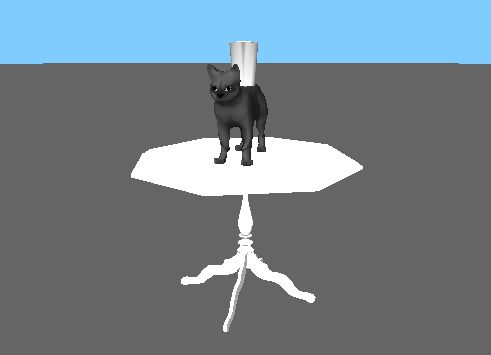
\includegraphics[width=\columnwidth]{wordseye.jpg}  
	 %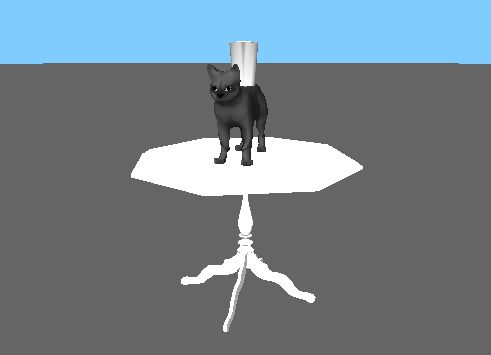
\includegraphics[scale=1.0]{wordseye.jpg}  
	 \caption[WordsEye.]{WordsEye rendering of ``The cat is on the table. The cup is
	 on the cat.''}
	 \label{figure:wordseye}
	\end{figure} 
	% ==============


Another example of text-to-scene generation is CarSim~\cite{Akerberg2003},
which uses a similar logical processing and rendering process, but is
specifically designed to deal with the recreation of car accidents by parsing
traffic accident reports. Where CarSim differs is that it tries to generate an
animated sequence by inferring the speed and direction of vehicles from the text
content. However, it is less concerned with the literal representation of the car, but
rather it concentrates on the situation surrounding the incident.

    % === Figure ===  
	\begin{figure}
	 \centering  
	 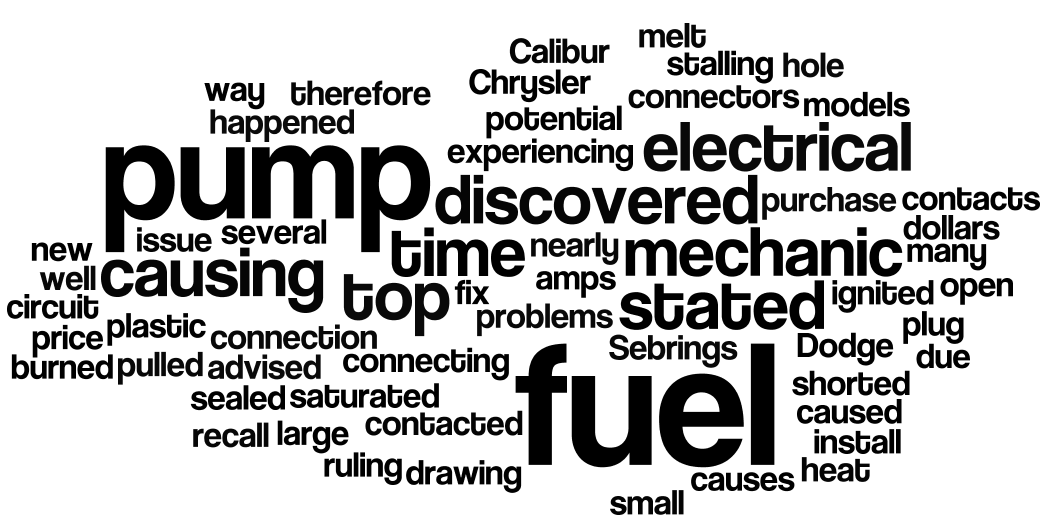
\includegraphics[width=\columnwidth]{wordle1.png}  
	 %\caption[Wordle]{A typical Wordle layout~\cite{VIE2009a}. \copyright 2009,
	 % IEEE. Reprinted with permission.}
	 \caption[Wordle.]{A Wordle rendering of a vehicle complaint report.}
	 \label{figure:wordle}
	\end{figure} 
	% ==============
 
 

%So far, the discussion have been around examples where the renderings are based
%on the literal meaning of the text. On the other side are interpretive
%renderings, where the images produced are not necessarily the ground-truth of
%the text, but often produced with artistic flares and particular theme in mind.

On the interpretive side, a popular example is the web-based application called
%Wordle(http://www.wordle.net). Unlike the systems mentioned above, Wordle does
Wordle~\cite{VIE2009a} (See Figure \ref{figure:wordle}). Unlike previous systems
mentioned above, Wordle does not perform any semantic inferences on the underlying text, it rather collects frequency
statistics of each word token and encodes the frequencies as font sizes.
Unlike the closely related tag cloud, Wordle offers more creative freedom in
varying typography and colours, which are all interactively chosen by the user.
Thus it is possible to create interpretive art works based on social and
cultural norms, for example using the green colour to represent topics about
money and finance. Later variations such as Tagul took this idea further by
binding the placement of the words to specific geometric shapes and outlines,
which further strengthens how people can create their own interpretations and
expose the underlying themes~\cite{tagul}. For example, a text article about
love can be place inside a shape of a heart, instilling the idea that it is
emotionally based. However, because these creations are not usually linked to
their original text, it can be questionable whether these are proper tools for text analysis. 
 

Another example is calligraphic packing~\cite{Xu2007}, which takes a more
liberal, artistic approach. This research visualizes single words by distorting
individual glyphs to fit into \twod regions. Creative freedom is given to the
people to choose which image best represents the word, as well as the amount of
acceptable distortion. However, due to concentration on artistic style, the
legibility of the actual words after the distortion transformation is not guaranteed.


%\textbf{Summary:} Unlike WordsEye and CarSim, we start with a scene that is
%pre-constructed, that is, we know ahead of time the subjects in our text 
%documents and can place them into \threed space. While it is interesting to use 
%grammatical approach to grab context, we found it more generalizable to use a 
%dictionary approach similar to Wordle for parsing text because we iterate 
%over thousands of documents.


%%%%%%%%%%%%%%%%%%%%%%%%%%%%%%%%%%%%%%%%%%%%%%%%%%%%%%%%%%%%%%%%%%%%%%%%%%%%%%%% 
\section{Non-Photorealistic Rendering}
Since the infancy of computer graphics, researchers have long been looking at
ways to render photorealistic images that are nearly
indistinguishable from a photograph taken by a camera. In recent years,
however, another area of computer graphics research has been looking in the
opposite direction: Non-Photorealistic Rendering. Non-Photorealistic Rendering can be 
described as any computer generated graphics that do not involve the accurate 
simulation of the behaviour of light. While photorealism has long been the holy
grail in graphics research, there are compelling reasons for using NPR
techniques. First, NPR images are judged based on their ability to
communicate a specific message to their viewers, thus they are driven to
emphasize features in a scene or some underlying attributes~\cite{Gooch2001}.
This is in contrast with photorealistic rendering where the goal is to compare
the rendering against a ground-truth image. Second, often times it is
undesirable to preserve a high degree of realism, reflections, shadows
and other natural lighting phenomena may obstruct or create
false-positive surface details. NPR can choose to ignore the natural laws of physics, and instead
choose to focus on different abstractions such that the illustration can be
meaningful to people from different fields. Since there are multitudes of
possibilities in NPR, this section solely focuses on prior works that related
to our work here, or served as our inspirations.

%\daniel{Perhaps repace toonshading with half-toning? more relevant because it
%mentiones textures} 

Images found in technically written materials, or those of
instructional manuals are quite different from those found in photo scrapbooks.
The key point, as stated above, is that communication is valued above realism. Early works by
Gooch \etal~uncovered common themes in technical illustrations and ways to
automate some of these properties~\cite{Gooch1998}. Gooch \etal~modified the
conventional shading algorithm to use a two-tone approach that shifts from
warm-colours to cool-colours, in addition, they added edge lines and removed
shadows. Illustrations created in this fashion have major benefits over
photography. One, strong lighting effects under the conventional shading model
are reduced, thus preserving the surface details under the light patches. Two, the
removal of shadow regions shows the hidden details that were not previously
visible. Other NPR shading techniques also exist, for example 
those that emulate the simplistic cartoon styles known as
cel-shading and toon-shading~\cite{Lake2000}. Generally speaking, cel-shading
and toon-shading map the intensity of light from a continuous function into discrete
values, creating distinct contours where the values change as if shaded by a
marker. Still other works look at the simulation of physical materials,
for example textures as halftones to simulate stylistic artistic
sketches~\cite{Freudenberg2002}, and pen-and-ink
illustrations~\cite{Salisbury1994}. However it is semi-automatic as some human
input is required for the right combination of textures, normal maps and other
special effects.
   

Another major benefit of NPR is that it can be used to simplify or
accentuate geometric features. By taking advantage of visual perception
capabilities of seeing continuities and surfaces as dictated by Gestalt Principals~\cite{WAR2004b}, humans can see and complete entire shapes with just a few
geometric primitives. Feature extraction, which revolves around the detection
and isolation of shapes and primitives, can be used to achieve this goal. 

%Feature extraction is one way to achieve this goal by
%simplifying an image down to geometric primitives of lines and curves.

Feature extraction can be done in either \twod or \threed spaces. The \twod
algorithm is image based, and based upon calculating the a discontinuity value
of a pixel against its neighbouring pixels~\cite{Gonzalez2002}. The
discontinuity can take on several types, for example colour, normal and depth. A
square matrix, called a kernel, is used as a convolution operator to evaluate a
measure of discontinuity of each pixel in the image. Any pixels with a
discontinuity measure that fall below a specified threshold are discarded, the
remaining pixels are collected and aggregated into higher level geometric
primitives. In \threed space, features can be classified under the broad
categories of ridges, valleys and  silhouettes.
Ridges are formed by two front facing polygons with dihedral angle between 0 to
180, similarly, valleys are front facing polygons with dihedral angle between
180 to 360, both of these are exclusive, as an angle of 0 or 180 results in a
flat surface. Lastly, silhouette edges are formed by the shared edge of
front-facing polygons and back-facing polygons. Raskar~\cite{Raskar2001}
computes these \threed features without connectivity information by extruding
additional faces per polygon. In addition, since the features are geometric
quads, additional processing can be performed on these quads such that they can
be rendered in a multitude of ways. However, because the extrusions are
performed on all sides of the polygon, the algorithm introduces extraneous
faces, which are hidden by existing geometries through back-face culling.
Hermosilla~\cite{Hermosilla2009} took this idea further by moving the extrusion
process to modern graphic pipeline's geometry shader, removing the need to perform 
the computations on the CPU. It should be noted that in an interactive environment,
geometric features are generally view dependent in both \threed and \twod
scenarios, and this usually means that feature extraction operations need to 
run on a per frame basis.
 

When it comes to expressiveness, NPR rendering styles can be used to convey a
variety of semantics. Of particular interest to us is the idea of uncertainty:
graphics that are visible to the viewer, but also convey a sense of error
and inaccuracy. Research in ancient architectural
reconstructions found that straight, solid
strokes convey a higher degree of certainty than strokes that are drawn faded and
curved~\cite{Masuch1998, Strothotte1999}. The relevance here to our work is
that we use this type of technique to convey objects that are not in the focused
context.


    % === Figure === 
	\begin{figure}
	 \centering  
	 %\includegraphics[width=\columnwidth]{copyright/viola.png}  
	 \includegraphics[scale=1.0]{copyright/viola.png}  
	 \caption[Importance-Driven Volume Rendering.]{Importance-Driven Volume
	 Rendering~\cite{Viola2004}.
	 \copyright 2004, IEEE. Reprinted with permission.}
	 \label{figure:viola}
	\end{figure} 
	% ==============

%One prominent research came from an
%importance-driven function that can be used to determine the visibility of
%objects~\cite{Viola2004} (See Figure \ref{figure:viola}). 

Another branch of non-photorealistic rendering deals with semantic segmentation
of objects in the scene, examples are illustrations found in science and
medical literature where specific parts are accentuated using different colours.
This is done in order to differentiate focus and non-focus regions in the final
illustration. These types of NPR techniques are particularly prominent in the 
Scientific Visualization community, where they deal with visibility issues to
ensure that semantically important objects are easily visible and to provide
features to deal with occlusion. For example, Viola \etal~used an
importance-driven function to determine the visibility of
objects~\cite{Viola2004}. In their work numerical scores
are assigned to volumetric components such that more important objects are
rendered more opaque than objects of lesser importance (See Figure
\ref{figure:viola}). A screen door transparency technique is introduced to
ensure overall visibility by rendering holes into the outermost volumetric
layers. The idea of segmentation and context is taken further by Tietjen \etal,
who describe a segmentation scheme that partitions different volumes into
focus, near focus and context categories~\cite{Tietjen2005}, with the following semantics:
\begin{itemize}[noitemsep]
  \item Focus object: Current focus and is emphasized.
  \item Near focus object: Object for understanding spatial location or
  interrelations.
  \item Context Object: All other objects in the scene.
\end{itemize}
The segmentation allows for further accentuation of specific regions, while
still providing enough background context to understand the subject matter.

%In action, focus, near-focus and context objects can be interactively changed
%and take on different artistic styles.



%%%%%%%%%%%%%%%%%%%%%%%%%%%%%%%%%%%%%%%%%%%%%%%%%%%%%%%%%%%%%%%%%%%%%%%%%%%%%%%% 
\section{Integrated Visualization}
Traditionally, Information Visualization deals with abstract data, while
Scientific Visualization deals with visualization of
concrete subjects such as physical or anatomical objects. However, while these
are two distinct communities, the division is not always obvious. Many
applications combine elements and techniques from both fields, though the two
sides remain separate disciplines. As data becomes more heterogeneous, new
approaches for data visualization make the case of whether the boundary should
exist or not, as illustrated by recent attention to discuss the similarities and
differences between the two groups~\cite{Hauser2005, Weiskopf2004}. The SciVis
community in particular has adopted techniques and practices that are
traditionally in the InfoVis community. A well-known example is the volumetric
visualization from Doleisch \etal, which uses multiple coordinated views in addition to 
linking and brushing techniques to further help the exploration
process~\cite{Doleisch2003}.

    % === Figure === 
	\begin{figure}
	 \centering  
	 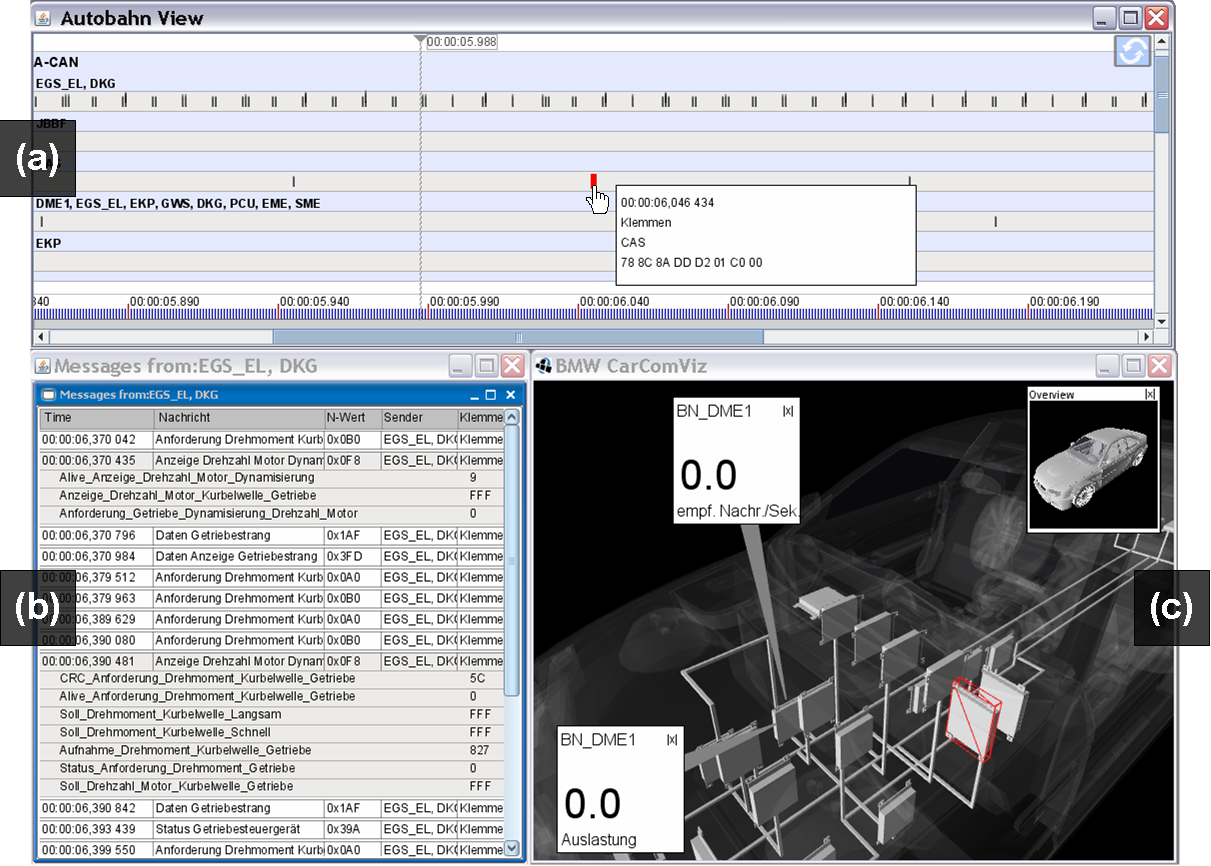
\includegraphics[width=\columnwidth]{copyright/sedlmair.png}  
	 \caption[CarComVis.]{User interface for CarComVis~\cite{Sedlmair2009}.
	 \copyright 2009, Springer. Reprinted with permission.}
	 \label{figure:sedlmair}
	\end{figure} 
	% ==============

For a more hybrid space approach between InfoVis and SciVis,  Balabanian \etal~
placed hierarchical renderings of human anatomy inside an interactive
balloon-tree graph~\cite{Balabanian2010}. In this graph, each anatomical object
occupies a node, and is arranged by logical hierarchy. The colours, size and arrangement of the nodes are dictated by abstract 
semantics, such as what is currently selected, filtering operations, 
and relations among the anatomical parts. The \threed rendering supports SciVis
operations such as viewing, slicing and picking of objects. Changes are linked
and propagated across relevant nodes and volume renderings.


In the InfoVis space, research by Sedlmair \etal~examined enriching
InfoVis visualizations with \threed models~\cite{Sedlmair2009}.
In this work, they presented two applications, CarComVis, which allows users to
explore intercommunication among vehicle components, and LibVis, which explores
environmental reading in a library setting. Neither one is explicitly about
physical objects, but contains inherent spatial information for reconstructing a
\threed representation: an automobile model for CarComVis and a virtual library
environment for LibVis. Sedlmair \etal~explore different types of integration
techniques, including the usage of multiple coordinated views and a total immersion 
environment where the user is in a virtual world. Subjective feedback 
from their study suggested a strong desire for integration of \threed
visualizations into traditional visualization and work flow. Our work in this
thesis is perhaps mostly closely associated with CarComVis (see Figure
\ref{figure:sedlmair}), however our renderings are driven by unstructured text,
and our interactions are directly applicable to the visualization itself rather
than through multiple coordinated views.

%\textbf{Summary:} We take an approach similar to CarComVis [Seldmair2009], we
%generated a virtual vehicle based on the components mentioned in our dataset. However, rather 
%than using a coordinated views for information seeking, our interactions are more 
%tightly coupled with the \threed visualization. Also, our visualization style is
%based on the context of the dataset, rather than using a fixed visualization.

%%%%%%%%%%%%%%%%%%%%%%%%%%%%%%%%%%%%%%%%%%%%%%%%%%%%%%%%%%%%%%%%%%%%%%%%%%%%%%%% 
\section{Focus+Context Techniques}
Focus+Context is a well-known and practiced technique in InfoVis; it is used to
draw attention to particular areas of interest while maintaining a certain degree of contextual 
information. There are various ways to discriminate these areas. For example 
Hauser reviewed the general approaches and demonstrated the usage of colour,
spatial-location, opacity, and other resource~\cite{Hauser2006}.
One interesting use of the focus+context technique is the idea of using lenses; the
lens traces back to a real world metaphor of a magnification lens, where the
area directly under the lens are distorted and enlarged by the optics. In
interactive visualization, the lens acts as a specialised user interface widget,
where the data graphics under the lens undergo a graphical transformation in
order to represent different semantics.


Fisheye Lens is a technique for enlarging
details on a \twod image, for example on digital maps and circuit
diagrams~\cite{Sarkar1992}. Much like its real world counterpart, a fisheye lens technique creates an ultra-wide viewing perspective that
creates a distortion displacement under the lens. The amount of displacement 
is controlled via a drop-off function that determines the degree of enlargement 
and shrinkage, typically with the central part of the lens enlarged while area
regions near the circumferences shrink to compensate. There are a
few usability issues with a fisheye lens, and likely the same issue applies to all
lenses that undergo geometric distortion: distorted graphics are more
difficult to read, and it is harder to tell where the focus is, because the
lens itself may occlude nearby objects which the viewer use as navigational cues.

Although not directly a focus+context scenario, the original publication of
using a flexible and multipurpose virtual lenses likely came from Bier \etal's Magic
Lenses~\cite{Bier1993}. The lens is composed of various widgets arranged on a
semi-transparent overlay, where the interaction with a widget affects the
immediate graphical region beneath it, for example changing the colour or size
of the graphical region.


%Although not directly a focus+context scenario, the original idea of using a
%flexible and multipurpose virtual lens likely came from research by Bier \etal,
%where a transparent overlay can be used to modify the appearance and behaviour
%of objects underneath the overlay panel~\cite{Bier1993}. Perhaps more
%significantly, the lens acts as an interactive layer, where actions can be send
%through the lens directly to the objects beneath it.


NPRLens follows up on the MagicLens metaphor from Bier
\etal, allowing users to interactively create images in a non-photorealistic
style~\cite{Neumann2007a}. NPRLens performs image processing on the \twod
projections of objects in \threed space. Graphical data points are first projected to screen space,
collected and aggregated into higher level graphical constructs such as line
segment and curve primitives. These can then be further manipulated such as
stretching, shrinking or changing the stroke styles of each primitive unit.


\threed MagicLens~\cite{Viega1996} is likely the first foray of the lens idea
taken into three dimensional space, and unlike the previously mentioned works,
MagicLens works with viewing volumes rather than \twod image maps. The lens in this scenario slices
the scene into different frustum volumes, each volume is then rendered separately 
and then recomposed together to create the final scene. This technique allows 
people to create interesting effects, for example exposing the skeletal 
structures of multi-layered objects. With more advanced hardware features, it is
possible to buffer the rendering into textures and combine them at a later
stage, rather than physically cutting the scene in volumes, this is the
technique that we use in our work.


Other than stylization and distortion techniques, the same lens metaphor can
also be used as a way to augment information seeking. In this context the lens 
is an exploration device that exposes hidden data points, or data points that 
cannot be feasibly displayed in a readable manner. Generally these cases arise
because of overlapping points, or when there are too many points on the screen,
making labelling of all points impractical as they introduce too much visual
clutter. Excentric Labeling~\cite{Fekete1999} uses the lens metaphor to deal
with densely populated data points on a \twod illustration. Data points are not
labelled, instead, when the lens is hovered over the locations that contain data
points, line segments are extended from the data points outward towards the
circumference of the lens. The actual text labels and descriptions are drawn
along the circumference, allowing viewers to make the connection between
graphics and text. The lens itself is movable which allows for exploration of
interesting regions. Extended Excentric Labeling~\cite{Bertini2009} (Figure
\ref{figure:bertini}) further extends on the idea by creating additional
interactions with the lens, dynamic overviews are shown inside the lens as
miniature graphs summarizing of objects under the lens. The labels are
scrollable to allow exploration of dense areas without overcrowding screen
space, the layout of labels and the extending lines are also altered to minimize
crossings which can cause additional visual complexity.
 
    % === Figure === 
	\begin{figure}
	 \centering    
	 %\includegraphics[width=\columnwidth]{copyright/bertini.png}  
	 \includegraphics[scale=1.0]{copyright/bertini.png}  
	 \caption[Extended Excentric Labelling.]{Extended Excentric
	 Labelling~\cite{Bertini2009}.
	 \copyright 2009, The Eurographics Association and Blackwell Publishing.
	 Reprinted with permission.}
	 \label{figure:bertini}
	\end{figure} 
	% ==============


%While both Excentric and Extended Excentric Lens operate in \twod space, there
%are some researches with that takes the same ideas into environments that are
%composed of \threed objects. 

While the techniques described above are largely applied to \twod applications, there are
applicable \threed focus+context techniques. Sonnet \etal~created a medical volume rendering system where the lens takes the form of a
\threed cursor~\cite{Sonnet2004}, although viewers cannot see into the cursor
itself, the cursor creates a spherical volume that pushes other volumetric objects away from the center, thus
creating more space for labels and annotations, and reduces the occlusion issues
that come naturally with \threed environment. Another system is BrainGazer, a volumetric visualization application that allows
users to draw a query path onto a segmented volume data~\cite{Bruckner2009}. The
path exhibits lens like behaviour, that is, the systems queries the objects that are in
proximity to the path drawn. Additional information about these objects is then
shown in a separate user interface panel. Our system uses a similar approach, in
that the scene we render is pre-segmented into regions of different
semantics, though we use an actual lens as the querying tool, and we deal with
geometric rather than volumetric data.

 
%\textbf{Summary:} Our approach to focus+context resembles a combination of
%approaches taken by BrainGazer, NPRLens and Excentric Labels. Like BrainGazer, we allow 
%people to form visual queries via indexing spatial location with different semantics, 
%though we take a proactive approach to highlight and link the text data back to 
%the visualization by combining ideas from NPRLens and Excentric Labels.


%%%%%%%%%%%%%%%%%%%%%%%%%%%%%%%%%%%%%%%%%%%%%%%%%%%%%%%%%%%%%%%%%%%%%%%%%%%%%%%%
\section{Design for Touch Interface}
As the cost of touch surface computing becomes cheaper, we are gradually seeing 
interactive surfaces introduced into public areas, office work environments and 
personal spaces. Interactive interfaces bring new possibilities of exchanging 
information in a walk-by scenario~\cite{Vogel2004}, allowing people to
interact with data without the need of peripheral hardware devices such as the
mouse or keyboard. Instead, people utilize their hands and fingers as
interactive mediums.

Though much of the work today deals with either collaborative or
distributed environments, the focus in this work deals with designing
surface-based gestures for a large display space. Gesture design
and classification have been looked at via crowd sourcing approaches,
leveraging public opinions to come to a consensus as to which action should be
associated with what gestures. For example, Wobbrock \etal~conducted
experiments where the consequences are given, and participants had to come up with their own appropriate gestures to cause the said
actions~\cite{Wobbrock2009}. Others, such as Hinrichs and Carpendale, looked at
how environmental and social context affect how people perform gestures
~\cite{Hinrichs2011}. In both cases, experimental results converge and they were
able to create high-level classifications. On the other hand, these
classifications are derived from independent, low-level tasks, where our
prototype looks at a specific problem from end-to-end. As such, these
classifications serve as inspirations rather than dictating our gesture
design.

Aside from classification, there are many other nuances and device specific
attributes in gesture design that one needs to pay attention to make them
more user friendly. Providing appropriate visual feedback, dealing with
false-positive/false-negative touches, and target acquisition are some of
important details for natural interactions. Much of the intricacies are outlined
by Wigdor and Wixon, where they discussed design principles and other
guidelines~\cite{Wigdor2011}.


 


%%%%%%%%%%%%%%%%%%%%%%%%%%%%%%%%%%%%%%%%%%%%%%%%%%%%%%%%%%%%%%%%%%%%%%%%%%%%%%%%
% This covers the problem analysis portion of the thesis
%
%%%%%%%%%%%%%%%%%%%%%%%%%%%%%%%%%%%%%%%%%%%%%%%%%%%%%%%%%%%%%%%%%%%%%%%%%%%%%%%%

\chapter{Problem and Analysis}
This chapter proposes our alternative approach for navigating a large body of
text. In particular, we introduce our dataset and problem domain: exploring 
vehicle complaint reports for reliability and safety analysis. We introduce our
goals and our requirement gathering process. Lastly we take a closer look at
our dataset records and specify the dimensions we want to visualize to support
our goals.

    % ===== Figure =====
	\begin{figure}
       \begin{center} 
       \begin{tabular}{c}
       \framebox[1\width ]{
       \begin{tabular}{l}
       The car is wandering sideways and you have to really control and \\
       focus on keeping the wheel straight to stay on lane. The best way \\
       to describe it is like you are always driving on windy weather \\
       with severe wind gusts. This happens on highway, with a speed of 60 \\
       MPH or higher. The assistant service manager said it could be the \\
       wheel alignment but after they aligned it and checked it, the problem \\
       remains. I live in an area where we get significant amount of snow \\
       during winter and I am afraid of my safety because of this problem. \\
       \end{tabular}
       } \\
       \end{tabular}
       \end{center}	
 	   \caption{An example of a complaint summary}
	   \label{figure:complaint}
	\end{figure}
	% ==================

%   % ===== Figure =====
% 	\begin{figure}
% 	   \centering  
% 	   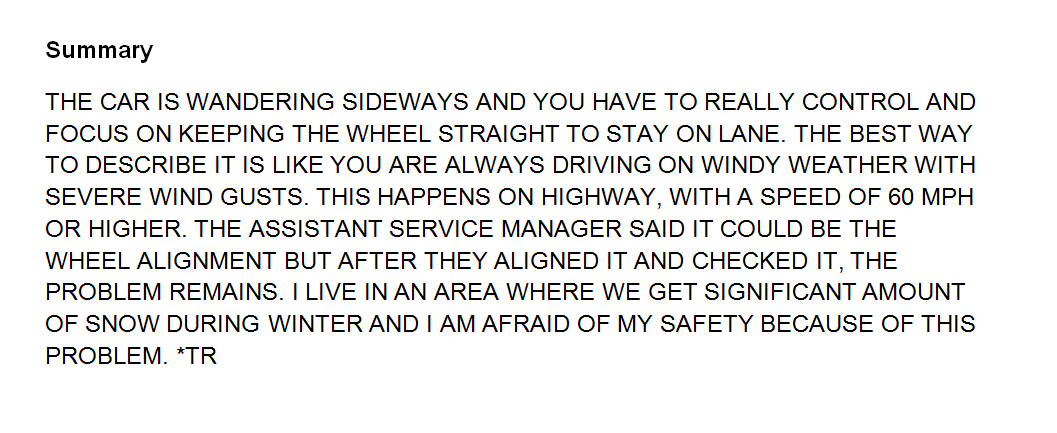
\includegraphics[width=\columnwidth]{complaint_text.png}
% 	   \caption{An example of a complaint summary}
% 	   \label{figure:complaint}
% 	\end{figure}
% 	% ==================


\section{Problem}
When it comes to navigating, exploring and querying large bodies of text,
traditional visualization techniques often approach the problem from an abstract
perspective. These techniques explores the context of words in the sentence of
the documents, for example Word Tree \cite{Wattenberg2008} allows people to
explore the most frequently occurring sentence structures within a document.
Other types of visualization looks at summarizing the underlying text, popular 
visualizations on the web today such as tag-clouds and word-cloud emphasize
the most frequently occurring words or phrases, thus revealing possible themes in
the text. Still, other techniques looks at the language semantics, for example 
DocuBurst \cite{COL2009a} spatially organize words based on the ``IS-A'' relationship.

Looking at the underlying semantics helps us understanding the content and 
themes in the text documents. However, there is another type of word context 
that is not fully explored in the visualization community. Within any text 
document which describes physical objects, each word that describes a 
tangible object has relation to its physical, real world counterpart. The 
entities also have relation to each other in terms of their respective 
spatial positions. For example, the sentence ``Automatic door locks when 
used, will not release from any of the four doors when engine is turned off.'' 
contains not only a co-occurrence relationship among the entities ``door'' and 
``engine'', but also relates to where the doors and engine are located on a 
real world automobile.

% Revealing these spatial relations of common words in text may enable new types of 
% insights and exploration techniques. By mapping physical entities onto virtual
% \threed representations it is possible to create a visualization environment
% that resembles the real world, the environment can then be explored and queried with relative ease
% due to existing familiarity of how these objects operates in real life. There are 
% many types of text that carries these sort of physically mappable vocabulary: 
% product reviews, technical manuals, maintenance logs, and our dataset: vehicle 
% defect reports.

Revealing the spatial dimensions has several benefits. Foremost, the
familiarity of the form makes the subject matter immediately recognizable
to experts and novices alike, combined with the message-carrying
capability of NPR illustrations, we argue that our approach is creates a
rich, engaging experience. Second, it is possible to conduct a different
type of data exploration: the spatial dimension allows us to explore
proximal relations and filtration by spatial volumes, possibly allowing
new insights to be formed.

So far, we are not aware of any exploratory visualizations which approach text
visualization by visualizing the real-world spatial context of the words in
text. Thus, our work looks at revealing these real world relations in a manner
that is useful for conducting text-analytic activities.

Consider product quality reports for a musical instrument. Visualizing
these report allows one to see exact location of the problems on the
3D model, for example: which valves are failing. Seeing the instrument
in physical form may promote conjectures that are less apparent
with text or abstract visualization, for example: perhaps the valves
failed because they are encased in a faulty housing. There are many
applicable datasets which carry this sort of physically mappable vocabulary:
consumer product reviews, technical manuals, and technical
support logs are examples.



\section{Use Case: Vehicle Complaint Reports}
We choose to demonstrate our approach on a dataset of vehicle complaint
reports. Each year thousands of reports are submitted to the
NHTSA database, consisting of consumer complaints, defect reports
and manufacturer recalls. Each report has fixed fields describing the
details of the incident (date, make, model, etc.), and a free-form text
field, typically containing several sentences which describe the incident
in detail, including what physical parts were damaged or broken. A sample of the
text description, which we use to drive our visualization, can be seen in Figure
\ref{figure:complaint}. Thus this data can be mined for frequency counts as
well as co-occurrence counts of car parts. All together the meta data and free
text offer a wealth of information on safety and reliability issues of
vehicles. Consumers can access this data online to support car-buying
decisions. The current interface uses a conventional search form, returning
long lists of textual results; there are no mechanisms to support
concise overviews or dynamic details-on-demand. 


 

% \subsection{Background and Requirement Gathering}
% One of the tasks for buying a vehicle is to examine the safety and reliability 
% of the vehicle. The NHTSA database offers a wealth of information to guide 
% purchasing decisions, as well as inform insurance companies and automotive 
% manufacturers about potentially serious safety and reliability concerns as reported 
% through experiences of real drivers in realistic scenarios. However, we have yet 
% to see any sophisticated ways of representing this dataset. Consumers have to
% use conventional search forms that returns a large number of amounts of textual
% results; there are no mechanism to support concise overviews or dynamic details on demand. 
% The step-by-step querying process also prevent  consumers from freely exploring 
% the data, they need to have a preconceived notion of what they want to look for, 
% thus likely prevent any type of unexpected discoveries.
% 
% On the other end of the spectrum, there exist consumer product website such as 
% Consumer Reports\footnote{http://www.consumerreports.org/} and
% Edmunds\footnote{http://www.Edmunds.com}. These website provide reviews and
% linear scale ratings for different types of vehicles, but these ratings seldom
% provide details and in-depth analysis. In other words, the ratings are too
% coarsely grained. Yet another issue with these websites is that they are
% typically targeted at newer vehicle models, as such, it can be difficult to look
% up and compare ratings between new and old models.
 
 
% \section{Tasks}
% While our data is temporal in nature and new 
% reports are constantly being added, our system is not, strictly speaking, a 
% real-time system that consumes streaming text data. Our system consume data in 
% batches, and to our knowledge, there are no known external facing API available 
% for monitoring updates. Having said that, our system share many of the same 
% concern as real time text streaming applications. Rohrdanz \etal
% \cite{ROH2011a} outline seven important tasks analytical tasks for working with
% text streams which we found to be suitable for our problem domain. These
% includes monitoring, decision making, change/trend detection, event tracking,
% historical retrieval, exploration and situational awareness.
% 
% For the purpose of analyzing vehicle defect reports, and for an audience of prospective 
% car/used-car buyers, some of the vital tasks are:
% \begin{itemize}[noitemsep]
%   \item Decision Making: ``Which vehicle should I buy?''
%   \item Historical Retrieval: ``Are there any major concerns with vehicle X over
%   the last 5 years?''
%   \item Exploration: ``How does vehicle X compare to other vehicles in the same
%   category?''
% \end{itemize}
% 
% From the perspective of an assurance engineer or incident investigator, the
% tasks may be:
% \begin{itemize}[noitemsep]
%   \item Monitoring: ``Are there any new complaints relating to vehicles of make
%   Y?''
%   \item Decision Making: ``Are there enough reports and evidences to warrant a
%   full scale investigation or a recall?''
%   \item Change and Trend Detection: ``For this type of vehicle, are the rate of
%   complaints per month increasing or decreasing?''
%   \item Situational Awareness: ``How does reports about my vehicle compare to
%   the current state of the automobile industry''
% \end{itemize}
% 
% In our design, we aim to create an application which aims to support these users
% and user tasks as they analyze these complaint reports. We take the view of the 
% consumer as the primary stakeholder. Thus, our goal is to provide text-analytic 
% visualization for helping consumers understand and explore vehicle safety issues, 
% which in turn will affect their purchasing decisions

\subsection{Requirements and Tasks}
In order to derive concrete requirements for our design, we needed to determine
the considerations which are most important to a consumer, whether for
purchasing for problem investigation.

We start our initial requirement gathering by looking at websites dedicated to 
vehicle owners and potential car buyers, our sources include expert columns, 
question and answer forums, car-buying tips and product rating websites such 
as Consumer Reports\footnote{http://www.consumerreports.org/} and
Edmunds\footnote{http://www.Edmunds.com}. 

Our findings revealed that, aside from the price factor, the next item people
care  about are safety and reliability.
This makes sense, purchase of a vehicle is a big investment, the vehicle itself 
needs to be reliable to be used frequently and ensure the safety of its passengers. 
In general, consumers want to know which brand/make they can trust. Other forum
posts refer to existing problems, with the owners asking whether the problem is an 
isolated event or if the issue is widely spread, this indicates a need and
willingness for detailed exploration. Car buying guides often advocate conducting thorough 
research on the vehicle and brand history, as well as leverage the experience of 
other owners. This is particularly important for used vehicles.
 
Based on these findings, we propose the following four design requirements for
our visualization prototype:
\begin{itemize}[noitemsep]
  \item R1: Provide an intuitive representation and make important items clearly
  visible;
  \item R2: Facilitate finding of trends, interesting facts and causal relations
  in the reports;
  \item R3: Allow multiple types of comparisons across different data
  dimensions;
  \item R4: Provide for reading of original complaint report text in the context
  of the visualization.
\end{itemize}

The types of tasks that we want to support are based on Rohrdanz \etal's seven
important analytical tasks for dealing with streaming data~\cite{ROH2011a}. 
Though the vehicle complaint dataset is not real-time it is temporal in nature
and shares many of the same concerns as real-time applications. The tasks are:

\begin{itemize}[noitemsep]
   \item Decision Making: Which vehicle should I buy? Are there enough
   reports and evidences to warrant a full scale investigation or a recall?
   \item Historical Retrieval: Are there any major concerns with vehicle X over the last 5 years?
   \item Exploration: How does vehicle X compare to other vehicles in the same category?
   \item Monitoring: Are there any new complaints relating to vehicles of make Y?
   \item Change and Trend Detection: For this type of vehicle, are the rate of complaints per month increasing or decreasing?
\end{itemize}


% \section{Data Dimensions}
% A typical complaint report consist of both structured and unstructured fields.
% The structured fields related to the type of vehicle and other explicitly 
% quantifiable variables relating to the incident (\eg, the odometer reading, 
% number of injuries, the incident location). The unstructured field is a
% free-form text field, it typically consist of several sentences describing the
% circumstances of the incident.
% 
% \textbf{Spatial:} Many texts contain spatial variables that can be mapped to the
% real, physical world. Sometimes these are explicitly stated, such as GPS 
% coordinates which are mapped to a specific location on earth, others, such as 
% an article about computer hardware, have implicit spatial locations in how the 
% described components are arranged with respect to each other. Visualization 
% offers a unique opportunity to gain insights about spatial patterns in a text 
% document by showing inherent spatial relations that are not apparent from looking 
% at the source text or their abstracted forms. For example, under Gestalt perception 
% of proximity, highlighted objects can naturally form clusters and other patterns 
% in \threed space, which can drive further analysis and exploration. Our spatial
% variables are the vehicle components, for example the engine, wheel and doors. 
% Like puzzle pieces, all together these component form a complete automobile.
% \threed visualization is not a trivial task, due to perceptual limitations it
% has many challenges when projected onto a \twod screen space
% \cite{WAR2004b}. However, a carefully designed \threed interface can also create a simple,
% compelling experience for people, particularly if the design goes above and beyond the 
% constraints of normal reality \cite{Shneiderman2003}.
% 
% \textbf{Time:} Time is almost omnipresent when dealing with streaming or reporting data, 
% whether it is the creation date or the timestamps within the document itself. 
% For our specific dataset, we suspect that much interesting information can be 
% gained by supporting high level activities such as seeing how a particular 
% object changes over time, and comparison of season to season statistics. Being
% able to search, compare and extrapolate trend information across time is vital for 
% understanding the underlying data, thus making time an obvious choice for our 
% visualization.
% 
% \textbf{Hierarchy:} The organizational hierarchy of the vehicle manufacturers
% (Manufacturer, Make, Model, Model Year) is an important aspect when purchasing 
% a vehicle. Consumers not only want to compare model-to-model in terms of 
% reliability and safety, they are also interested in whether the manufacturing 
% companies are producing reliable vehicles in general and how manufacture rank 
% with respect to each other. The organization hierarchy present a natural 
% progression from the most general selection down to specific models, and thus 
% supports successive refinement of queries. Note that the selection of 
% organizational hierarchy as a data dimension is a problem specific decision, 
% it does not generalize to text analytics for other domains.



%%%%%%%%%%%%%%%%%%%%%%%%%%%%%%%%%%%%%%%%%%%%%%%%%%%%%%%%%%%%%%%%%%%%%%%%%%%%%%%%
% This chapter describes the text processing steps
%%%%%%%%%%%%%%%%%%%%%%%%%%%%%%%%%%%%%%%%%%%%%%%%%%%%%%%%%%%%%%%%%%%%%%%%%%%%%%%%
\chapter{Data Processing}
The data is received a a textual list of records consisting of meta data about
the complain and the text description of the complaint. We apply several
processing steps to each document to first extract the physical entities
keywords, and then to calculate the semantic scores. For this dataset, we have
chosen the semantics of occurrence relations and co-occurrence relations. Finally we
segment \threed models to match our keyword ontology. Each of the steps are
explained in greater detail below.


\section{Creating Entity Keywords}
Our entity extraction process leverages the WordNet database, a lexical English
database that stores nouns, verbs, adjectives and their relations among each
other \cite{WORDNET}. In order to get a comprehensive list of physical entities, we use the meronym 
relation in WordNet. A meronym describes a ``part-of'' relationship between two 
nouns, for example, a brake is a part of a wheel, and a wheel is a part of the 
automotive vehicle. All together, the meroynomy relationship forms a hierarchical 
structure where the most general part forms the root node, while the most specific 
parts form the leaf nodes. We use two common words pertaining to cars to bootstrap 
the hierarchy : ``car'' and ``vehicle''. From this we extracted two tree
structures rooted at ``car'' and ``vehicle'' respectively, we then merge the two
hierarchies, assuming that ``car'' and ``vehicle'' are equivalent. 

\subsection{Formulation}
Before any logical processing can take place, we spent some time doing
preliminary analysis, looking at the data text, their format and how they have
evolved over the life span of the data repository. We performed several
normalization tasks: One, we used regular expressions to convert the text, which
is call caps, to regular case format. Secondly, we remove suffix characters that
appear at the end of the text paragraph, that, as far as we know contributes
nothing to the incident context. Although we changed the underlying text, the
normalization process improves readability, and allows us receive meaningful
output from natural language parsers.

The first issue was to devise a method for extracting physical entities; a
document can contain multiple entities, but not all of which are related to the 
subject matter. On top of that, many entities can have implicit hierarchical 
relations, such as relation between component and its subcomponents. This 
relation is important because it enables logical groupings which are useful for
high level overviews.

While this process extracts a fair amount of physical entities, an analysis of
sample dataset showed that it is not representative of the entities being
mentioned in the documents. The primary reason for this is due to the use of synonyms in the documents, 
where the entity words in question are using an alternative names. To alleviate
some of these confusion, we additionally extract the synset relations from WordNet. A
synset is a set relationship that describes words that are semantically
equivalent of one another, for example ``limo'' and ``limousine'' both describe
the same type of object and thus belongs to the same synset group. For each word
in our current collection, we replace it with its respective synset.

The addition of synsets into the vocabulary gave us a comprehensive number of
keywords, however it also created undesirable noises. Manual examination of data
sample reveals that there are still disconnects between the dictionary
vocabulary and real world vocabulary. The next section we will describe how we
overcome these issues.

    % ===== Figure =====
	\begin{figure}
	   \centering  
	   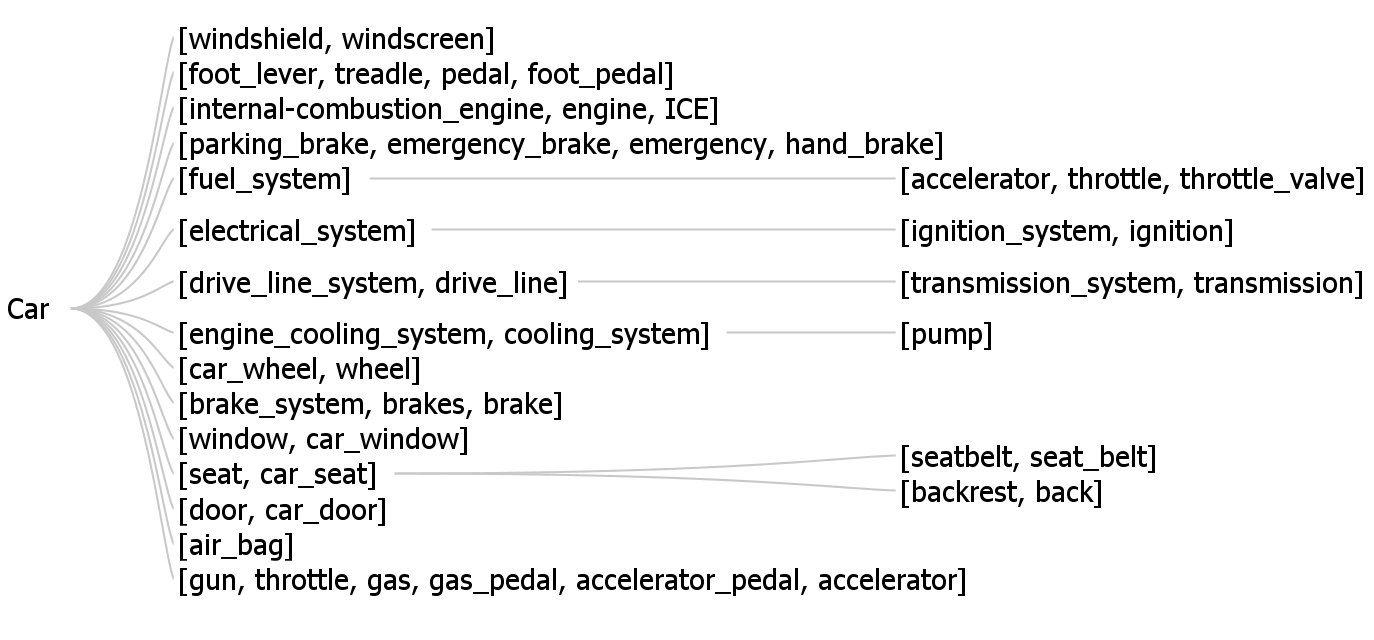
\includegraphics[width=\columnwidth]{meronomy.png}
	   \caption{An example of the meronomy plus synset structure}
	   \label{figure:meronomy}
	\end{figure}
	% ==================


\subsection{Enhancement}
As an additional step to augment our keyword vocabulary, we perform two manual
steps:
\begin{itemize} [noitemsep]
  \item Removal of nouns that are too generic from the vocabulary.
  \item Preprocess the documents and mine for any missing nouns.
\end{itemize}
The first step deals with the removal of keywords that are not considered to be
physical objects under typical usage, for example WordNet hierarchy of a
vehicle contains ``first'', ``second'', ``third'' and ``fourth'', which
describes the first, second, third and fourth gears respectively. Including
these words will likely result in over-counting the number of occurrences of
gears because they are used in every day speech. We also removed several
acronyms that will likely cause ambiguities, for example ``ice'', which is short for internal-combustion-engine,
will cause issues if the document is about ice, the solid state of water. They
are therefore removed from the keyword dictionary. 

The second step deals with any possible missing keywords that are not in WordNet
meronyms. We attempted to detect these semi-automatically with natural language 
processing techniques. We first perform part-of-speech (POS) tagging on our document 
corpus. POS taggers look at the grammatical structures of text and break down 
sentences into lexical categories such as nouns, verbs and adjectives. We use the 
POS output and tie them back to the original text, extracting the nouns and 
compound-nouns. We perform this step for all the documents in the corpus and 
count the number of occurrences for the nouns and compound-nouns. We then manually 
exam the top occurring nouns and add them into the hierarchy where we believe 
would be appropriate.

\subsection{Limitations}
While we believe this extract process is a plausible method for building the
vocabulary, we acknowledge that WordNet is not the definitive authority for our 
problem domain, nor would it be for any specific domain. The automatic
extraction can be used as a starting point. The keywords vocabulary should be
extended and further refined by consulting experts that works in the problem field. 



\section{Semantic Relations}
We chose to look at two semantic relations in our dataset: occurrence and
co-occurrence. The occurrence relation is a measure of how frequently a
particular entity was mentioned throughout the corpus, and is an
indication how important the entity is overall. The co-occurrence relation is
also a frequency measure, it measures how frequently an entity is mentioned along
with another entity in the same document, indicating possible causal relations.
For example: ``Engine failed because radiator overheated'' has a co-occurrence
relation between engine and radiator.

Semantic relations are document-entity pairs, that is to say, there is a
one-to-many relation between a document and our keyword ontology. Detection of
keywords in document is done through a tagging process. In the sections below we
describe this process in detail, as well as formalizing the semantic scoring
function.


\subsection{Tagging}
We use straight forward string matching to tag each document. First, document
text is segmented into word tokens, then for each token we perform a string
match against the entity keywords. When a match is found, we store a triple
that describes the document identifier, the keyword and the position of the word
in the document. In the aforementioned example above, we would store (Doc0,
engine, 0) for the engine entity, and (Doc0, radiator, 3) for the entity
radiator.

In the actual string matching, we use an open source, off the shelf snowball
stemmer\footnote{http://snowball.tartarus.org/} to normalize each word token. 
Stemming is a process of reducing the words to their root forms. Finding the
root is important because it unifies the singular and plural forms, as well, it
converges various forms without the need to add additional vocabulary to our
keywords. We performed stemming on both the word tokens as well as our keyword
vocabulary.

For the document text, stemming is performed on all string tokens and not
limited to nouns. This has both positive and negative effects. In our data, 
there are many word tokens with both noun and verb forms, for example ``braking
malfunction'' can be correctly associated with the keyword ``brake'' with
stemming. On the other hand this also introduced false positives, the word
``lock'', which refers to the component, is falsely picked up when the text describe components
``locking up''.

We have also looked at tagging explicit casual relations. Using the dependency
parser extension, the output is a tree-like structure that can be used to infer
word dependencies. In practice this did not work very well; informal languages,
spelling mistakes and grammatical errors result in incorrect dependency parse
trees. We ultimately opted to go for a more general approach, where we tag each
physical entities as well as co-occurring entities within the same document.


\subsection{Scoring}
Once all documents are tagged, the occurrence and co-occurrence scores can be
computed. 

% Once we have identified the entities in each document, we can compute each
% entity�s importance score. We denote the importance score of a physical entity 
% as the number of times it is mentioned within the document corpus. We have two 
% variations of importance score: occurrence  and co-occurrence. Within our
% problem context, the occurrence scores denotes the components that are most prone to failure, while 
% the co-occurrence suggest causal relationships among the objects.

Let G be a (possibly empty) set of objects that are in the keyword hierarchy and
c be a single object in the hierarchy. We define a scoring function S(c, G) to be 
the total number of documents that have at least a single mention of c and G. Thus 
when G is the empty set the score is the occurrence score (every document 
contains an empty set). When G is non-empty the score reflects the co-occurrence 
strength among a set of components. For clarity we illustrate this with a few examples:
\begin{itemize} [noitemsep]
  \item $S(engine, \{\})$: The absolute strength of ``engine'' component in all
  documents
  \item $S(engine, \{engine\}$): The strength of ``engine'' relative to
  ``engine'', thus the same as the above
  \item $S(engine, \{brake\})$: The number of times engine keyword is mentioned
  when brake keyword is mentioned as well. Thus, mathematically,  $S(brake,
  \{\}) \geq S(engine, \{brake\})$
\end{itemize}

Each document is only counted once per physical entity, this was done to
discourage biases coming from longer documents where the entities are
repetitively mentioned.

Unlike the tagging process, scores are not stored, but rather
evaluated on a need basis. The numerous combinations of G along makes it
impractical to persist the scores in any manner, as the number of possibilities
is a permutation of all available entities.
 
 
\subsection{Limitations} 
For this prototype, we gave the same score weighting to each objects. This is a 
subjective measure because not all parts are created equal. For example: if window 
is mentioned 10 times and the engine mentioned a single time, does that mean we 
should pay more attention to the window component? A simple extension to this
work would be to devise an appropriate weighting scheme by consulting the domain
experts. 

Another limitation is the vocabulary set itself, while we are only storing nouns 
as keywords, it would be interesting to look at verbs as well. For example, 
``stalled'', ``stalling'' are typically associated with engine object. Adding
verbs into our dictionary would give more flexibility and accurate results.


\section{Model Segmentation}
We use geometric models that compose of triangular mesh groups, where each mesh 
group can be uniquely identified and semantically mapped to our keyword ontology. 
The segmentation is done manually, with consultation of car schematics when it 
was not clear where the parts located. Where the model is missing parts, 
we add placeholder geometries.

We have chosen to use a sedan model as the starting point of our visualization. 
This was chosen based on the fact that sedans are the most common class of 
vehicles and best represent our data. We acknowledge that different types of 
vehicles may have different spatial arrangement of their components, we hope to 
remedy this as more vehicle models are processed.


%%%%%%%%%%%%%%%%%%%%%%%%%%%%%%%%%%%%%%%%%%%%%%%%%%%%%%%%%%%%%%%%%%%%%%%%%%%%%%%%
% This chapter covers the design aspects, primarily on visual design and
% touch interactions 
%  
% - Should probably talk about active versus inactive versus context objects 
%   in the 3D visualization section
%%%%%%%%%%%%%%%%%%%%%%%%%%%%%%%%%%%%%%%%%%%%%%%%%%%%%%%%%%%%%%%%%%%%%%%%%%%%%%%%
\chapter{Designing Descriptive Non-photorealistic Rendering}
This chapter covers our visual design process and the rationales of our
design decisions. The system interface, as seen in Figure \ref{figure:overview},
is composed of four major components:


\begin{description} [noitemsep]
   \item [3D Visualization:] The central view of the visualization system
   is a stylized rendering representing the physical entities in the text documents,
   the visualization can be zoomed and rotated to explore different viewing
   perspectives. Each entity is rendered with respect to a function which denotes
   its importance. We explore different rendering styles to take advantage of
   viewers' preattentive perception, allowing them to quickly uncover the
   important information.

   \item [Lens Widget:] The lens widget is a detail-on-demand tool. It is used
   to specify spatial regions on the \threed visualization. Entities under the
   specified space are considered to be in focus, and more information about
   these entities is shown beside the lens as heatmaps.

   \item [Heatmap Widget:] The heatmap displays time series data at the lowest
   granularity level in order to provide trend and pattern analysis. It is
   organized into a grid; each cell is shaded in accordance with its score of
   that time period. In addition, the heatmap identifies the entity names and
   their raw numerical scores.
   
  \item [Document Widget:] The document widget displays the source text documents.
  The panel displays documents relating to the currently selected objects and
  highlights all relevant keywords.
\end{description}

 
In addition, two domain specific widgets provide filtering functions to
visualize subsets of the text corpus. These widgets are created from the
metadata in the documents, they are:

\begin{description} [noitemsep]
  \item [Time Widget:] The widget is composed of two independent range sliders
  with different granularity: year and month. The widget allows viewers to
  adjust the time range for the visualization. Accompanying each range slider is
  a histogram showing the accumulated volume of complains over a time period.
  The widget itself is placed at the top-left of the display space.
  
  \item [Hierarchy Widget:] The hierarchy widgets are placed at the
  top portion of the display as a series of drop-down menus.
  The hierarchy widgets allow successive refinement of dataset by means of
  filtering on organizational hierarchies. Going top down, the system supports:
  Vehicle Manufacturer, Vehicle Make, Vehicle Model and Vehicle Year. The hierarchy
  widget is also used to select two different vehicle types when making
  comparisons.
\end{description}

 
    % === Figure ===
	\begin{sidewaysfigure}
	 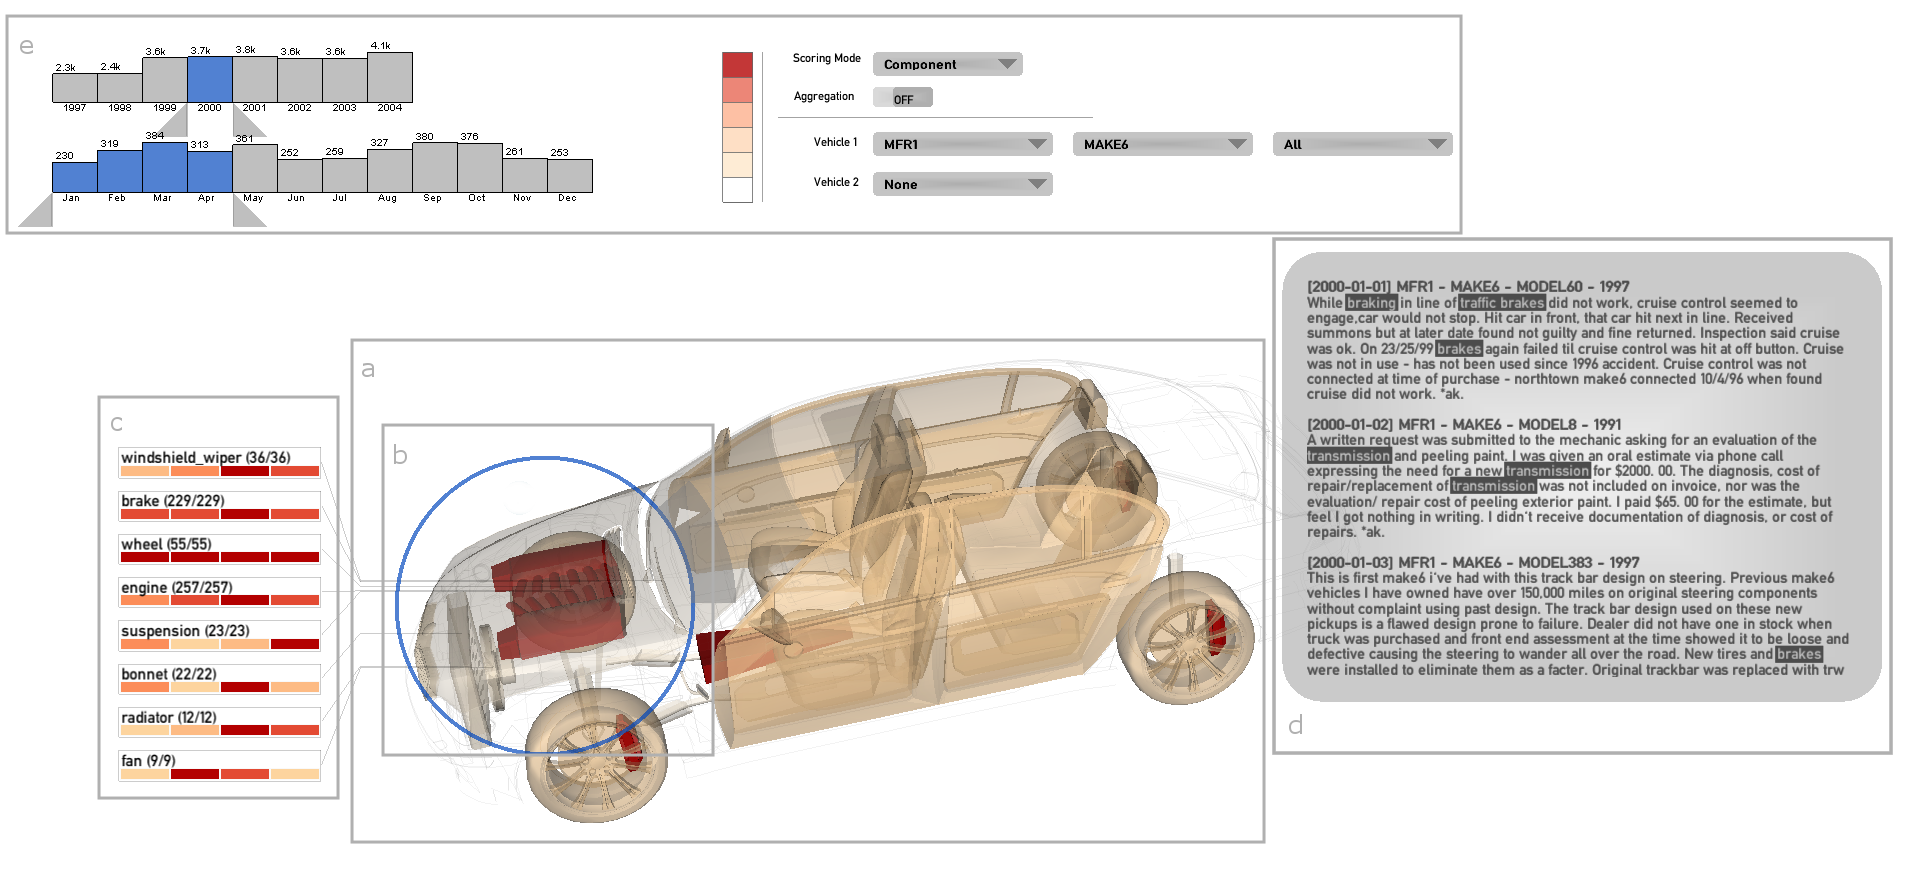
\includegraphics[width=\columnwidth]{overview_2_annotated_2.png}
	 \centering  
	 \caption[Interface Overview]{System Overview: (a) The 3D visualization, (b) lens widget, (c) heatmap widget, (d) document widget, and (e) filters. }
	 \label{figure:overview}  
	\end{sidewaysfigure}
	% ==============  

The following subsections will describe each visualization components in
greater detail, with respect to how each widget works and their design trade
offs.


\section{3D Visualization}
This section describes how to perceive the \threed visualization, how it was
designed, and discusses various design trade-offs.

\subsection{Rationale}
A major part of our design for this thesis is the mapping of abstract semantics
onto realistic looking \threed models. But this can also be a source of
complication. We have to deal with the additional difficulties of navigating in
three dimensional space as well as work around perceptual limitations. So why
use \threed models in the first place? Familiarity with the models and varied
exploration methods were key motivations. The familiarity with how the physical
entities look in real life means people do not have to learn additional visual
mappings. Communication may be easier because there is a shared common ground
among the different parties involved. Proximal relationships are also easily
perceived if they have realistic spatial mappings and can encourage more
thorough exploration of the dataset. These advantages are not readily present in
abstract representations, while with careful design it is possible to overcome
many of the pitfalls of perceiving \threed graphics. Lastly, we are not merely
mimicking \threed objects, our visualization goes further to facilitate user
oriented tasks~\cite{Shneiderman2003}. We enhanced the rendering process with
NPR techniques, along with interactions to explore the \threed space in an intuitive manner. 

Yet another argument is that the use of a set of \twod images can also convey
realism. Our opinion is that they lack the expressive power and playfulness of a
fully rendered \threed model. Flat image representation would likely result in
multiple images, used to cover different viewing perspectives. Mentally integrating 
them could result in more cognitive load due to viewers having to switch between images to
see different data.


\subsection{Visual Mapping}
Because our visualization environment makes use of three dimensional space,
extra care is taken into account for the selection of visual variables. Not all 
visual variables are appropriate: shape, position, and orientation are inherently
used to represent the geometries on the virtual model, a double encoding of these
variables, is likely going to lead to confusion, compromising the ability to
interpret the visualization, or destroy any resemblance of the virtual model to
its real world counterpart. Therefore such variables were rejected as ways to encode the score. 
Size is an interesting variable since in theory size can support most of the
characteristics. However, it is implied that all the objects of the same value have the equal size, 
which is certainly not the case for physical objects with sub components. One also needs to have
a mental image of the original size before encoding takes place. Colour 
and value variables are not used to represent the virtual model, since
they are not a part of the  basic geometry building blocks of vertices, line-segments, 
and polygons. We found colour and value to be appropriate for our visualization, 
although they do not provide a sense of quantitative measure, the capability to see ordering, 
make selections and associate similar colours and values makes them a logical choice for an
overview visualization.

Lastly, textures present an interesting option, textures can carry additional 
characteristics, particularly descriptive attributes. It may be possible to use 
textures to simulate certain effects, for example a rusty surface. Nonetheless,
textures do not possess inherent ordering or quantifiable characteristics and thus were not
included in our design. However it may be interesting to use textures for
visualizing individual document semantics; we leave this idea as future work.

\subsection{Stylized Rendering}
In order to enhance the message carrying capacity of the visualization, we
considered several NPR techniques as a medium to create  more expressive
illustrations. We associate the entity score with either an NPR technique, or use
the score as a parameter into an NPR function. In accordance with our
requirement, the encoding scheme should be clear and distinguishable by visual
examination (R1) while maintaining the real world aspects. Our effects include
varying stroke, halo/glow, colour variations, and transparency effects.

We chose colour mappings as our primary visual encoding which denotes the
strength of non-zero score entities, and use other techniques to denote
selection and overall context.

Designing a colour scheme for the encoding of the virtual component objects
presented several design trade-offs. We colour each object by mapping its score 
to a linear diverging yellow-orange-red hue scale, which is further divided into 
six discrete scoring bins. While this setup has a limited granularity, it is
easier to accurately perceive a small number of discrete colours than viewing a continuous
scale~\cite{WAR2004b}. We mitigate any ambiguities that may arise with the discrete scale by
providing numerical values with the lens and heatmap widget, which we discuss later.


\threed geometries may not be visible due to occlusion or containment.
The first case can be partially solved by altering
the viewing distance and viewing perspective on the visualization, whereas in
the second case no amount of viewing adjustment will solve the occlusion issue.
To address this problem, we double encoded the score as both the
colour and transparency values. The transparency value of each geometric object
is proportional to the entity�s score, such that the higher scored entities
appear more opaque, while the lower scored entities appear more transparent. The
maximum and minimum transparency values are capped between 0.4 and 0.8 such that
no objects are completely opaque or completely transparent. Our transparency scale
is slightly weighted to give more emphasis for more frequently occurring
entities. One challenge of rendering translucent geometries in \threed space is
that the ordering of geometries becomes important for alpha-blending to work
correctly; out-of-sequence geometries can lose their depth cues when blended
together. We discuss this effect, and solutions in further detail in the
implementation chapter.


The zero score has a special semantic in the visualization. When an entity's
score is zero, this indicates that there are no known references of the entity
in the documents. Not rendering them would reduce visual clutter, but comes at a
cost of not having a background reference, which gives visual cues to not only
what viewers are looking at, but also the placement and relative position among
other entity objects. To show that these components are semantically different
than others, the system renders them with silhouette styled edges in a just
noticeable colour so they are visible but not overly
distracting~\cite{BAR2007a}. It is worth noting that zero scored objects only
provide graphical context, they do not partake in any user interactions.



 

\subsection{Selection}
Selection of entities is used to refine the visualization scope, for example
selecting the windows entity tells the system to only visualize documents that
refer to windows. The system provides several methods for selecting entities:
selections can be made by directly interacting with the \threed visualization,
or through interaction with the heatmap widget.

    % === Figure ===
 	\begin{figure}
 	 \centering  
 	 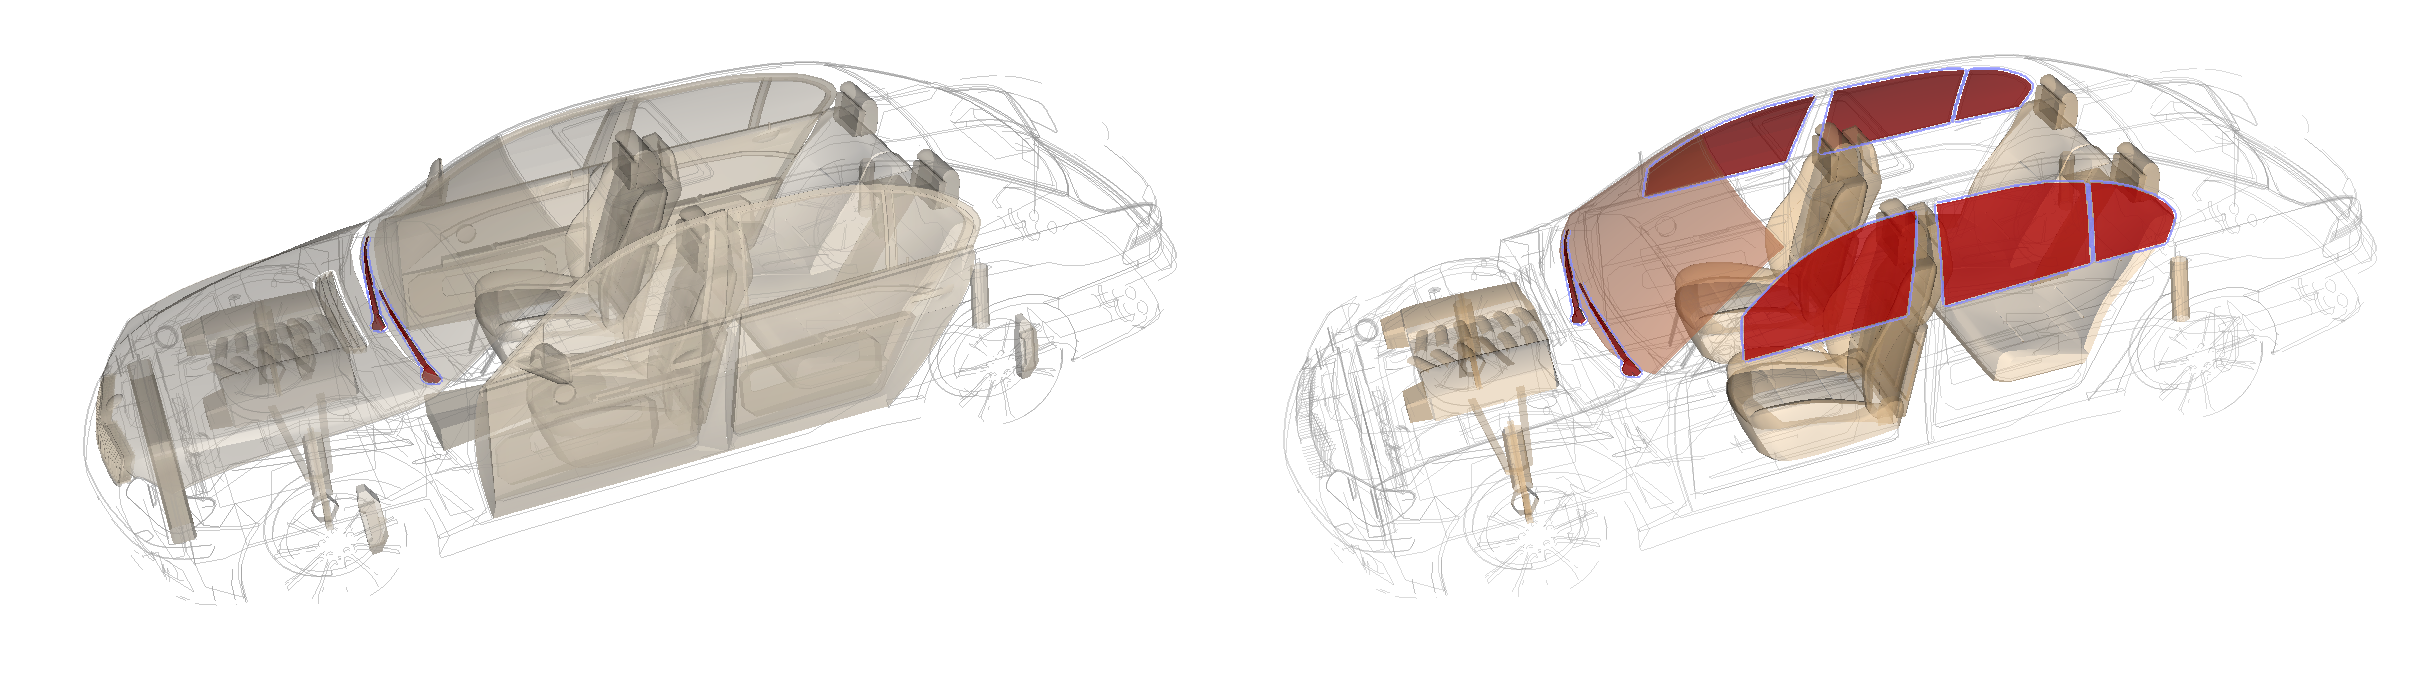
\includegraphics[width=\columnwidth]{select.png}
 	 \caption[Interactive Selection]{The visualization changes to reflect
 	 co-occurrence relations. Left: showing co-occurrences with respect to
 	 windshield wiper. Right: showing co-occurrences with respect to both
 	 windshield wiper and window entities.}
 	 \label{figure:selection}
 	\end{figure}
 	% ==============

By default, the application has no entities selected, thus the visualization
reflects the absolute number of occurrences of each entity. As
selections are made, each entity's score is recomputed to show co-occurrence
relations with the selection. Note since selected objects
fully co-occurs with themselves, they are promoted to the highest bin.
In this manner, high correlations are red and highly opaque, while low
correlations are yellow and highly transparent. For example, if a person selects
the windshield wiper, the visualization is rerendered to show entities
that co-occur with the wiper component and the strength of this
relation. If the same person then selects the windows, the visualization
will show co-occurring relation to both windshield wiper and windows. This example
is reflected in Figure \ref{figure:selection}. The rerendering process is
facilitated by an animated transition that interpolates the graphical effects.


% Entity objects can be acquired in two ways: One can directly select the entity
% by performing the tap gesture on the \threed representation, or tapping the
% heatmap through the lens widget. In the case where objects occlude each other
% in \threed space, direct selection will return the object that is closest to
% viewing point. In order to select occluded objects, the scene can be
% rotated to reveal hidden entities. Alternatively, we can use the lens� depth
% functionality to cut away occluding geometries, or directly clicking on the
% heatmap representations which are always available.
% 
%     % === Figure ===
% 	\begin{figure}
% 	 \centering  
% 	 \includegraphics[width=\columnwidth]{interaction_select.png}
% 	 \caption[Interactive Selection]{The visualization changes based on the
% 	 currently selected entities.}
% 	 \label{figure:selection}
% 	\end{figure}
% 	% ==============
% 
% Selection is toggle based. When an entity is selected, we apply a blue borderb
% to the associated heatmap and the line segments that links the heatmap back to
% the visualization. To visually accentuate the selection in \threed
% space, we employ a halo like effect around the hull of the mesh objects. Both
% selection and deselection of any entity triggers an event to recalculate the
% entity scores, an animated sequence then starts to interpolate the colour of
% each \threed object to reflect the scoring change.
% 
% The re-evaluation of the entity scores are based on current selection,
% specifically they are recalculated based on their co-occurrence relation with
% the current selection. Thus, highly co-occurring entities will score higher and
% be more visible than lowly co-occurring entities.
% 
% Selection of an entity with zero score is considered invalid, instead, the
% system will propagate the selection event through the zero scored entities.
 
%\daniel{Stopping here\ldots}

\subsection{Trade-offs}
We recognize that blending different hues in \threed space does not necessarily
produce a result which preserves the original hues, and can potentially lead to
distracting visual artifacts. Different hue preservation schemes
exist~\cite{Chuang2009} but were not implemented for this prototype due to the
added performance complexity (hue adjustments are performed at per pixel level). Subjectively, 
we did not find any visual distractors and thus decided that this was not necessary. A 
single-hue scheme with varying saturation and opacity was tried as well, but we
found it less eye-pleasing and lacks the \emph{pop-out} effect that is more prominent on multi-hue 
colour schemes. 


%Due to known issues with blending, we have tried to use a single hue grey scale 
%with varying brightness, but we found that it was somewhat difficult to distinguish 
%overlapping or contained objects. Subjectively speaking, single-hue also looks
%less aesthetically pleasing, the entities did not have the ``pop-out'' effect
%as we seen with multi-hue schemes. Thus we decided that using  a multi-hue
%scheme was more appropriate, despite the potential blending artifacts.

A second design trade-off was whether lighting effects should be used. Lighting
effects such as specular lighting can create distractions because it can create 
highlights in places of little or no significance. Without any realistic
or simulated lighting effects, the visible colour of the components exactly
matches the colour assigned to the score and as seen on the legend.
However, without any type of lighting, particularly some type of diffuse lighting, 
the \threed nature of the model, and the details of various components are not
sufficiently visible. Adjacent objects that share the same score appear to be glued together 
as a single component; adding boundary outlines helps but creates undesirable
visual clutter. When lighting effects are enabled, the objects are easily
distinguishable as lighting provides a clear silhouette. However, this type of lighting modifies 
the colour based on the incidence angle of the light rays, thus it no longer matches 
the assigned colour. Ultimately, we decided that the benefits of objects recognition and
familiarity outweigh the colour offsets. The results of our design choices can be seen in
Figure \ref{figure:visualEncoding}.

%Ultimately our design decision is that object recognition and 
%familiarity is important to us. Thus, by restricting the number of hues (6 buckets) 
%and using soft white light, we contend that the lighting effects do not disturb 
%the colour perception enough to obscure which hue-bin the component belongs to. 
%We made the design decision that the benefits of enabling lighting to visually 
%resolve the components outweighed the negative effect of shifting colours away 
%from those displayed in the onscreen legend. The results of our design choices
%can be seen in Figure \ref{figure:visualEncoding}.
 
 
    % ===== Figure =====
	\begin{figure}
	   \centering  
	   \includegraphics[width=\columnwidth]{visual_encoding.png}
	   \caption[Trade-offs]{Showing the visual design trade offs. Top left: single
	   hue with flat shading. Top right: multi-hue with flat shading. Bottom left: single
	   hue with lighting effects. Bottom right: multi-hue with lighting effects. The bottom right
	   was selected as the final design; parts are not distinguishable in the top
	   row, while the bottom left did not have a strong pop-out effect.}
	   \label{figure:visualEncoding}
	\end{figure} 
	% ==================


Since the system visualizes \threed geometry, it can be
tempting to apply other types of techniques. For example we attempted to encode the importance and other 
numerical semantics into a geometrical distortion function that can be applied
directly onto a \threed mesh. In practice, this does not work well for visual evaluation:
in general, objects are of different shapes and sizes, applying a small distortion 
is not entirely obvious while a large distortion can destroy the familiarity of 
the form. It is also more difficult to recognize objects under distortion and to 
compare the degree of distortion among objects.


%Yet another problem is that it is not possible to order or quantify by 
%shape \cite{BER1983a}, which makes the distortion a qualitative measure instead
%of a quantitative one. In addition, the ability to read quantitative value from a 
%distortion field presumes that the viewer has a mental model of what the object 
%looks like without any distortions, an assumption that we cannot make with our 
%intended audiences.  However distortion remains an interesting possibility because 
%we may use distortion to visually paint the action words, testing this will be 
%part of our future work.




\section{Lens Widget} 
Using a metaphor of looking through a magnifying glass to reveal better details
about a specific subject, we created an interactive lens widget to extract and
show detailed information about entities in the text documents. With respect to the information
seeking process, this approach combines both filter and detail-on-demand phases.

The lens widget operates in a hybrid \twod and \threed space: the lens itself exists
on a flat \twod plane and it casts a cylindrical querying volume into the scene.
When the lens is positioned over the visualization, each entity object is tested to see if its 
corresponding meshes are in the lens' querying volume. We use the centroid to do the inclusion
test, though more accurate, albeit slower methods exist using
image-based algorithms~\cite{Ali2005}. Entities that are under the lens' area of
focus have detailed information, shown as heatmaps on the left and right side of
the lens widget. Connecting line segments are drawn from entities to their
heatmaps to show association: first the heatmap is connected back to the lens'
circumference, then from the circumference back to the entity's projected centroid.


    % ===== Figure =====
	\begin{figure}
	 \centering  
	 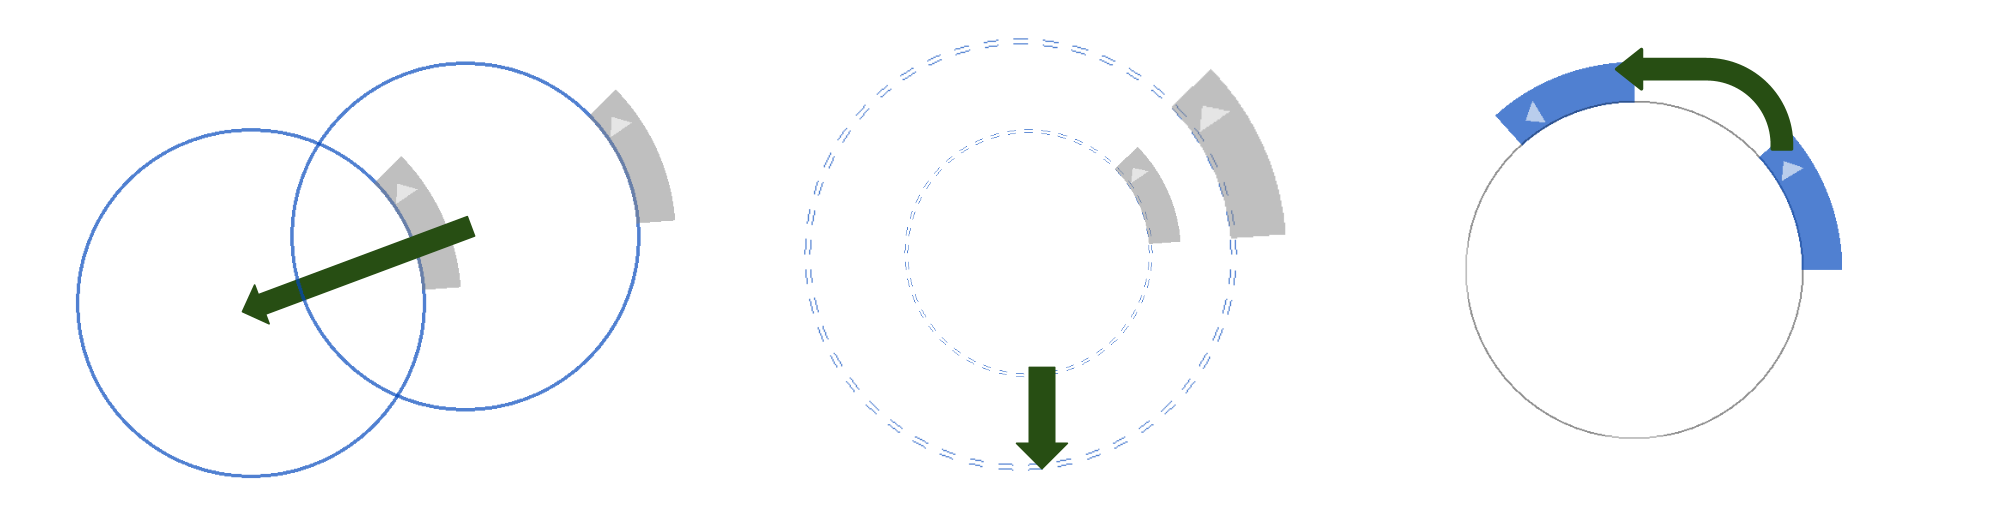
\includegraphics[width=\columnwidth]{lens_interaction.png}
	 \caption[Lens Interaction]{Interactions, from left to right: moving the
	 lens, resizing the lens and adjusting the depth handle.}
	 \label{figure:lens_interaction}
	\end{figure}
	% ==================


    % ===== Figure =====
	\begin{figure}
	 \centering  
	 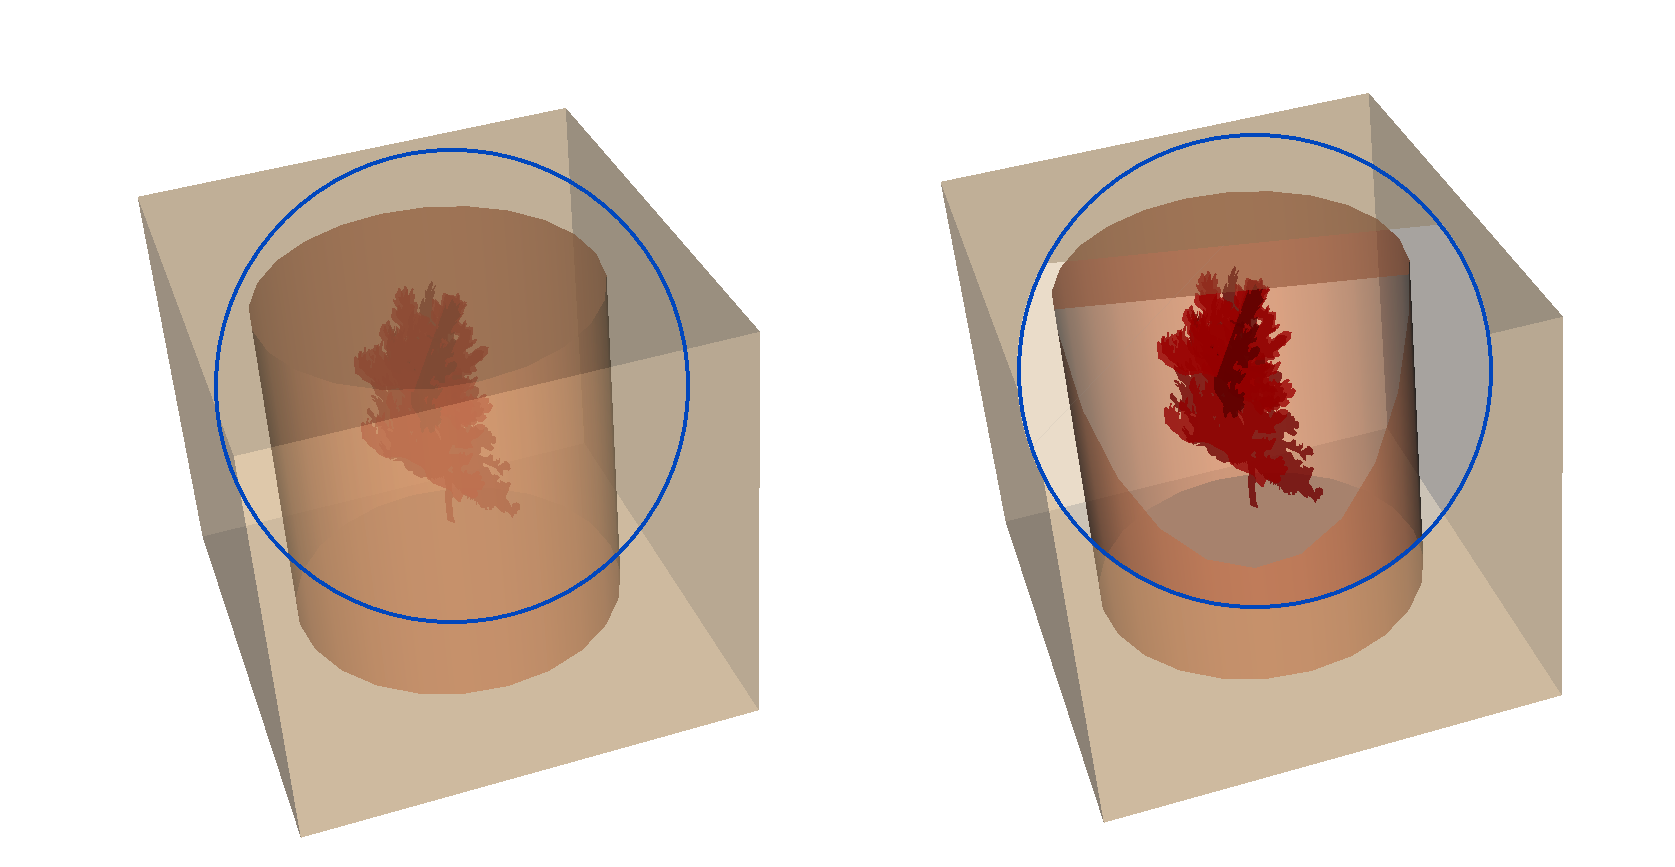
\includegraphics[width=\columnwidth]{lens_example.png}
	 \caption[Lens Depth]{The lens widget can be tuned to expose
	 occluded geometries. Left shows the unaltered geometry. On the right, the
	 lens cuts into the geometric shapes to expose the tree contained in the
	 cylinder, which itself is contained in a box.}
	 \label{figure:lens_depth}
	\end{figure}
	% ==================
	
	
The lens widget utilizes its own rendering pipeline: object geometries
are sent into the pipeline as normal, rendering results are 
then stored in an intermediate buffer and later combined in fragment
shaders with the default scene. This is an independent
process, and thus allows us to render the lens� scene with a different rendering
style and semantic. To visualize the lens widget itself, we
draw a semi-transparent border around its circumference so viewers
are aware of its extent. When interacting with the lens widget, the
widget becomes active and the system renders the border blue, otherwise 
the default grey colour is used. The semantics of rendering within the lens is not impacted by
whether the lens is active or inactive.	

 

The lens enables three different actions, seen in Figure
\ref{figure:lens_interaction}. The position of the lens can be moved by dragging
within the lens, impacting the currently focused entities and the heatmap charts. The lens can be resized by
dragging on the border of the lens, increasing or decreasing the query
area. Lastly, the depth plane can be adjusted by rotating the depth
selector tab around the circumference of the lens (see Figure
\ref{figure:lens_depth}). The depth plane function provides a method for people
to reduce occlusion, as all entities that are the cut by the plane are drawn in
an outline style, allowing viewers to see through them and into the object. Objects that
are cut off are excluded from any scoring calculations, they also have
their heatmaps hidden to reduce visual clutter. These three interactions
can be combined together to create a rich, flexible query mechanism.


Multiple lens widget allow for simultaneous exploration of
different parts of the visualization. For example, if the subject matter is of
an elongated shape, it is possible to use two lenses to explore the entities
positioned at either end. However, no semantics are currently defined for
multiple lenses to co-exist in the same spatial location, that is, the lens widget
has no defined behaviour when it is overlapped with another lens.


\subsection{Spatial Interaction}
Traditional systems use explicit queries as a mean to
communicate with the underlying data such as through structured forms and search boxes. 
While this works well for task analysis, it has an implicit assumption that the person knows something about how the
system works, and how the data is structured. Thus it can be a limiting factor
that prevents a wider audience from using applications without prior training.

In this thesis we take a different approach. More specifically, the lens widget allows people to
demand and filter detailed information by means of a visual query. Unlike explicit queries,
visual query is performed more passively by moving the lens widget about the 
visualization. Points of interest, if any, are shown as heatmap charts without
explicit requests. Thus a user is free to roam about the visualization without 
any specific goals or prior knowledge about the data, making the visualization
more playful and open to unexpected discoveries.

%\daniel{Maybe cite the bohemain bookshelf would be appropriate here}


In addition to the freedom of exploration, the lens has an additional 
benefit of allowing people to specify spatial regions. Imagine the case where 
a person is asked to investigate issues relating to the ``front'' of the 
vehicle. This query is difficult to formulate: components situated at the front 
need to be identified (which inconvenience  a person with novice expertise), 
and ``front'' itself may be subjective depending on the person. By repositioning 
and resizing the lens, a person can identify the front, back, or any other
spatial region quite easily.




\section{Heatmap Widget}
The heatmap is an interactive widget that shows entity-specific information over
the selected time frame. Each heatmap is designed to communicate how the volume
of complaints changed over time for individual entity components by fitting 
time series data onto a two dimensional grid. In this system, the heatmaps
allows year-to-year and month-to-month comparisons.

% Prior to our heatmap implentation, we have also considered using a simple 
% scatter-plot approach, with time on the X-axis and the volume of complaints on
% the Y-axis. While this solution is simpler to read and likely easier to detect
% long term trend, its major drawback is that it is likely more difficult to
% make seasonal comparisons. For example, imagine a case where we want to compare
% summer to fall over a 4 year span, one must constantly make the context switch
% to decipher which parts of the graph represents summer, and which parts
% represent winter. Also, in extreme cases scrolling need to be utilized for very
% long time frames.

    % ===== Figure =====
	\begin{figure}
	 \centering  
	 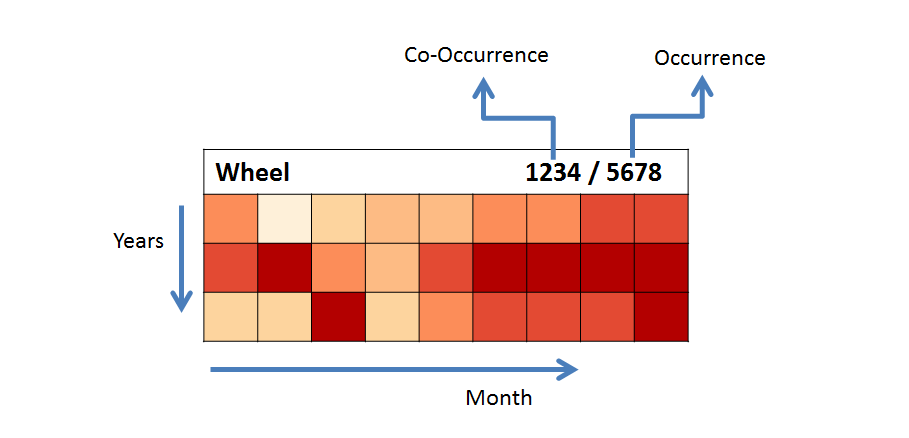
\includegraphics[width=\columnwidth]{heatmap2.png}
	 \caption[Heatmap schematic]{Heatmap schematics}
	 \label{figure:heatmapSchematic}
	\end{figure}
    % ===================

The time segments are arranged chronologically onto a grid like a calendar,
the months are arranged left-to-right in ascending order, and the years arranged 
top-to-bottom in ascending order (see Figure \ref{figure:heatmapSchematic}). The dimension of the heatmap's grid corresponds to 
the selected time on the time widget. Each cell then represents the entity score for
the particular month. We use the same 6-bin colour encoding for the heatmap
widget to keep a consistent colouring scheme throughout the system. The heatmap
label, placed at the top of the widget, shows the entity name, co-occurrence score 
and occurrence score. Note the choice of the entity name is the first word in the 
keyword's synset, which may differ from the words used in the document. For example,
the heatmap would display ``engine'' if ``internal combustion engine'' is in the text.

When examining the heatmap, trends and outliers can be detected visually. The
grid-like view aligns both months and years spatially, allowing viewers to
make yearly (row-to-row) and monthly (column-to-column) comparisons with relative
ease. Two types of interactions are supported by the heatmap widget. Selecting the 
heatmap is equivalent to a selection on the \threed visualization. Performing a hold
over an individual cell toggles a tooltip that displays the numerical score for that
cell, a blue border is drawn around the cell, the same border is linked over all cells
of the same month across visible heatmaps, allowing for a quick comparison.


\subsection{Layout}
With respect to heatmap placement, we have considered two
types of layouts around the lens widget: A flush-left/flush-right layout
that places the heatmaps on either left or right side of the lens, and a radial
layout where each heatmap is placed around the lens� circumference. 

The radial layout uses the centre of the lens as an anchor point, heatmaps are 
positioned around the lens by extending an imaginary line from the anchor 
point through the entity centroids to the circumference. The result is eye-pleasing,
however the layout turned out to be unstable in practice: any lens movement, whether
it is horizontal or vertical, may cause the heatmaps to slide along the circumference 
or swap positions with another heatmap. This layout behaviour made comparison and tracking 
difficult and thus was rejected.

%The radial
%layout is eye-pleasing, but is unstable during movement transition due to a
%single anchor point in the centre, and it is harder to compare across heatmaps
%because they are not spatially aligned, thus it was deemed unsuitable. 

For the flush layout, we first sort the object centroids by their 
Y-coordinates in screen space, then we place the heatmaps on
left/right side based on the heuristics below: 
\begin{itemize}[noitemsep]
  \item Heatmap placement should always be outside of the axis-aligned bounding box of the entire \threed model.
  \item If the entity centroid is closer to the right edge of the bounding box above, it will be placed on the right, else left.
  \item If the heatmaps are off the screen space, pull them back to the edge of the display so they are visible.
\end{itemize} 
Since there is no reliance on the centre of the lens for placement, movement of the lens widget will not cause
drastic changes and thus is more stable when moving the lens over the visualization.

Due to limited display space, not all heatmaps are shown at once. A scrolling mechanism, shown
as up and down arrows on the lens, are used to scroll through unseen entity objects; numerical
indicators on each arrow provide a summary of how many entities are hidden in either direction.
We set the maximum visible heatmaps to eight in this system.
 

\section{Document Widget}
The document widget is the final stage of our drill-down process by providing links 
to the raw text (R4). Each document is divided into two sections:
the header section shows each document's meta attributes and the content
section shows the raw text descriptions. We denote the selected entity words and
co-occurring entity words using blue and grey highlights respectively to create
contrast against the remainder of the text. Scrolling is enabled when text
content overflows the display panel. A document widget in action is seen in
Figure \ref{figure:document}.

    % ===== Figure =====
	\begin{figure}
	 \centering  
	 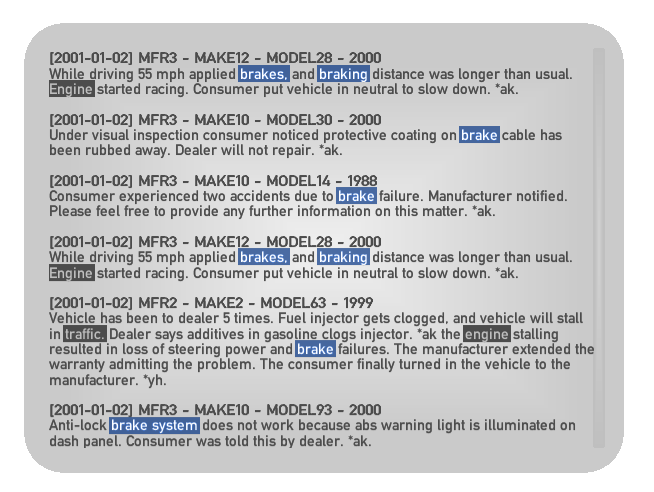
\includegraphics[width=\columnwidth]{document_2.png}
	 \caption[Document Widget]{The document widget, the words highlighted in blue
	 are selected. The words highlighted in grey are the co-occurring entities}
	 \label{figure:document}
	\end{figure}
    % ===================

The document widget is toggle-based and is by default hidden from view to save screen space. 
Once activated, an animation will expand its dimension from a single pixel to its full size at the
activation coordinate, a reverse animation is used to deactivate the panel. Once
fully visible, the document widget embeds itself with two different interaction
regions. The left region, which takes up 80 percent of the panel, is used for
relocating the document widget to a different position. The right region is
designated for scrolling through the documents.





\section{Data Filters}
In this section, we describe the time and hierarchy widgets. These are used to
model the fixed fields (date, make, model, etc.) in the complaint documents.
They are domain specific and are used to filter data into logical
subsets. See Figure \ref{figure:filterFull} for a close up of our data
filters.

    % ===== Figure =====
	\begin{figure}
	 \centering  
	 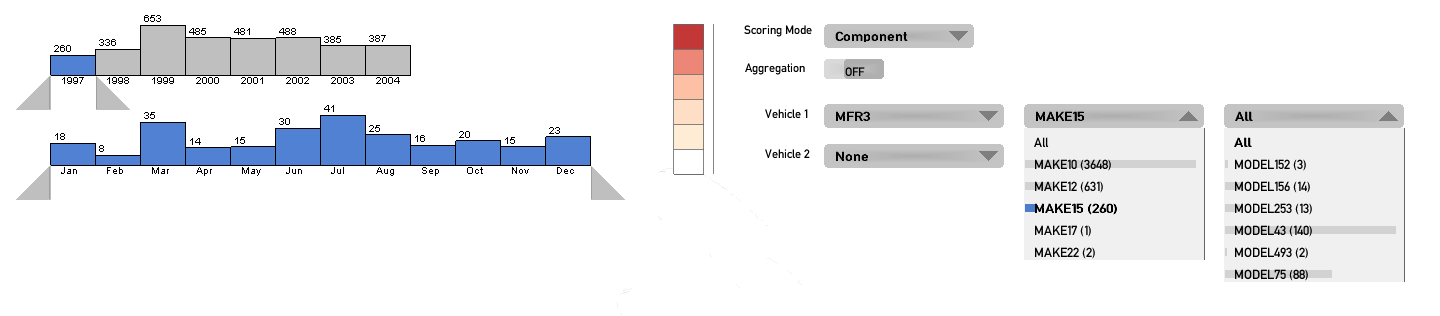
\includegraphics[width=\columnwidth]{filter_full.png}
	 \caption[Interactive Filters]{Interactive mode. From left to right: time widget, legend and hierarchy widget.}
	 \label{figure:filterFull}
	\end{figure}
    % ===================
    
 
    % ===== Figure =====
	\begin{figure}
	 \centering  
	 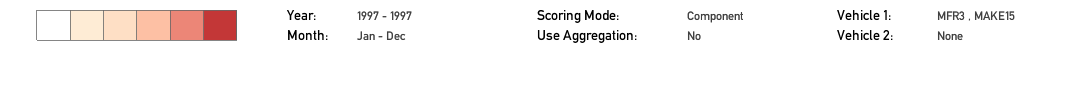
\includegraphics[width=\columnwidth]{filter_compact.png}
	 \caption[Compact Filters]{Compact mode. From left to right: legend, time widget and hierarchy widget.}
	 \label{figure:filterCompact}
	\end{figure}
    % ===================  
    
\subsection{Time Widget}
The time dimension is encoded as a histogram, with the height of each bar denoting 
the volume of unique complaints for that time period. There are several granularity 
options with our document collection: daily, weekly, monthly or yearly. From an 
analysis of the incoming volume of documents, we found that daily and weekly 
granularity levels resulted in too much noise, these are discarded in favour
of months and years.

The widget is made up of two sliders. The top slider represents time
period in years, and the bottom slider represents time periods in months. 
Labels at the top of each bar give the numerical representation of the volume of
documents, note for the month slider the volume is the accumulated sum across
selected years. Markers at the bottom of each slider are used to select contiguous 
blocks. Selections of months and years are independent, for example, a person
can select January to June, between 2000 and 2005. This selection behaviour allows
people to focus and filter based on seasons and other sectional based divisions.

Interactions with the sliders are done through dragging their markers as mentioned above, or directly
on the histogram bars. A double tap action on the year slider's bar provides a shortcut
to select the entire year. An animated transition is used to interpolate the
height of the histogram bars.    
    
\subsection{Hierarchy Widget}
The hierarchy widget is designed to model inclusive relationship, in particular,
it is specifically designed to address the need for comparison (R2) and trend
finding (R3). For our problem domain, this relationship is represented as the
organizational hierarchy. Our data contains four such fields: manufacturer,
make, model and model year. For example: Honda (Manufacturer) owns Civic (Make). 
These widgets are shown as a variant of the combo boxes which
supports single selection, each item in the widget shows the name and the number
of documents associated with this organizational level. Rather than having the
readers comparing items by reading the numbers in text format, we double-encoded
the number of documents as a horizontal histogram in similar style as the scented
widget approach~\cite{Willett2007}. The bar for each item in the widget is shaded
in light grey, and turns blue when the item is selected. 

Each level of the hierarchy is shown in an individual widget. We position the
widgets left-to-right across the display space, from the most general to most
specific classification. Each widget's content is 
dependent on the selection made on its parent. For example, the ``make''
selection widget will contain different makes if ``GM'' is the selected manufacturer than
it would for ``Chrysler.''  Non-top level hierarchy widgets remain hidden from view 
until it has selectable content, thus at the start, only the top level 
(manufacturer) widget is visible.








\subsection{Compact View}
The system provides a compact panel that encapsulates the legend, time and
hierarchy widgets as a work-around to create more screen spaces for the main
visualization. As seen in Figure \ref{figure:filterCompact}, the compact view
removes much of the interactive GUI elements and replaces them with textual
summaries placed across the top of the display. It allows viewers to zoom in
closer on the \threed visualization and place interactive widgets in spatial positions that would have
otherwise caused occlusion issues. A swipe gesture is used to toggle between the 
two views.





%%%%%%%%%%%%%%%%%%%%%%%%%%%%%%%%%%%%%%%%%%%%%%%%%%%%%%%%%%%%%%%%%%%%%%%%%%%%%%%%
%\daniel{talk about waiting when making a selection}

\section{Design for Touch Surface}
Touch-enabled systems can be deployed in situations that are otherwise cumbersome
for systems that use mouse/keyboard input. For example, a
walk-up-and-use scenario in a public place or within a meeting in an office
setting. Our visualization is designed for these settings where traditional input devices may
not be available, in particular the visualization system is suited for large touch
displays. In this section we describe the gesture and interaction designs.


\subsection{Semantic Zones}
Zones are used to segment our display space and to process touch events. 
Each zone consists of one or more polygonal defined areas with
predefined semantics for handling touch-based gestures. In the event that the zones overlap
each other and the system receives an event, the event will be propagated to the zone
with the highest priority, the remaining zones will ignore the event. The priorities are 
fixed and predetermined.

When a touch point is registered by the sensor hardware, the coordinate of the
touch point is checked to see which zone it is in, a coupling is created to
identify the touch point with a specific zone, the coupling will remain until
the touch point is removed. The reason for this approach is to allow higher error tolerance, we
want to avoid sudden changes of semantics which would defy user expectations.
This approach allows a subset of our dragging gestures (lens handle, slider
makers, and scrolling) to continue to execute even if the actual touch point is
moved off the predefined areas.

In the list below, we summarize the different zones in the system:
\begin{itemize}[noitemsep]
  \item Visualization Zone: The main visualization, handles selection
  and deselection semantics of \threed objects, as well as heatmap selection.
  \item Time Zone: Covers the year and month time sliders 
  \item Filter Zone: Covers the organizational hierarchy widgets 
  \item Lens Zone: Handles semantics for change the physical attributes of a
  lens widget
  \item Document Zone: Covers the document widget
  \item Empty Zone: An empty zone is a specially designated zone that is none of
  the above. Empty zone handles gestures related to camera and miscellaneous
  functions.
\end{itemize}

The priority of the zones are in reversed usage order. The most data specific
widget, the document widget, has the highest priority, followed by lens, and the
visualization zone. The remaining ones have the same priority as they have
static positions.
 

\subsection{Gesture Design}
While we tried to adhere to commonly accepted gestures for navigation and
selection based tasks, our gesture design is also influenced heavily by the  
hardware and the perceived usage scenario: an infrared sensor overlay placed
atop a large, nearly vertical display screen. The hardware setup has several
design implications. The infrared sensor is imprecise because it senses
movements that are near the display instead of real touches, as such it is possible to introduce
false positives due to hand posture and orientation. Software heuristics can be
used to mitigate the consequences of these untended noises, however,
there are ambiguous cases where software logic cannot guarantee the correct
outcome. For example, imagine a single handed gesture with the thumb and index
finger, we have noticed through experimental trials that the knuckles on the
other fingers are often picked up as extra touch points as well due to their
proximity to the sensor. In this case, it is difficult to tell which points
are intentional without additional information such as camera or depth image. 
As the sensor provides only the XY coordinates, we cannot infer hand orientations. Thus, we decided
to abandon any complex, explicitly-singled-handed, multi-fingered gestures in
favour of a simpler, less error prone-approach.

The final gesture set is  an accumulation of several design iterations.
At each iteration, fellow lab members were asked to pilot-test the new gesture
recognitions and heuristics, their reactions and feedback were then incorporated 
into the next design iteration. 

Within the current iteration, there are two types of basic touch gesture semantics: 
a short-touch and a long-touch. A short-touch consists of any gesture
where the initial position is held for less than a threshold of 450 milliseconds, 
while a long-touch is held for longer. The threshold is derived from the pilots
studies.

Using the short-touches and long-touches as building blocks, we
constructed a more complex gesture set: 
\begin{itemize}[noitemsep]
  \item Touch/Tap: A short-touch followed by disengaging the gesture.
  \item Hold: A long-touch followed by disengaging the gesture. 
  \item Drag: A short-touch followed by some movement.
  \item Drag-Hold: A long-touch followed by some movement.
  \item Swipe: A fast drag event.
\end{itemize}

Gestures are designed to be discrete and cannot be transitioned from one to 
another. For example, a dragging gesture to change the selected months cannot 
be transitioned to making a selection on the \threed visualization without lifting the hand.

Below we summarize the system's interactions:
\begin{itemize} [noitemsep]
  \item Perspective Manipulation: Perspective manipulation consists of the rotation
  of a \threed model and camera zoom. Rotation is achieved with a
  single point horizontal or vertical drag gesture, which corresponds to
  rotation of the XZ and XY planes. Zooming events are triggered by bringing
  together two touch points closer together or further apart. Zooming gestures are similar 
  to ``pinch'' and ``spread'', however the points are much further apart than normal to avoid the problems of
  singled-handed multi-finger gestures. All perspective manipulations must start in the empty zone.

  \item Entity Selection: Entity selection is triggered with a single tap on the mesh
  representing the entity or on the entity's heatmap.
  
  \item Tooltip: A hold gesture, or drag-hold gesture over the heatmap's cells will toggle the tooltip. 
  
  \item Lens Manipulation: A lens widget is created by specifying its diameter
  with two hold points, for example using index fingers on left and right hand
  to create the diameter. We impose a minimum and maximum diameter length to
  keep the physical size of the lens within reason, with our display hardware,
  we use the range between 100 to 500 pixels. Dragging gestures performed on the inner part
  of the lens shift the lens' location, while dragging gestures performed on the
  border resize the lens with respect to the point's distance away from the
  centre. A resize that results in a diameter that falls below the minimum
  threshold removes the lens widget all together. The handle tab on the
  widget adjusts the depth parameter, dragging the handle counter-clockwise
  increases the cutting depth, while the reverse decreases the cutting depth. We
  modelled this behaviour after the zooming mechanism on the barrels of camera
  lenses.
  
  \item Text Browsing: The document widget is toggled with a hold gesture over 
  the  empty zone. An active document widget has two zones, the left-most 80 percent
  of the document panel is used for reposition, while the right-most 20 percent for scrolling.
  Both  reposition and scroll actions use the drag gesture.

  \item Hierarchical Widget: A single touch gesture is used to open, close and to
  make selections. Scrolling is achieved by performing a vertical drag gesture on the item list.
  
  \item Time Widget: Single touch gesture is used to send select events to
  individual time sliders. Dragging gesture is used to move the slider markers.
\end{itemize}

    % === Figure ===
	\begin{figure}
	 \centering  
	 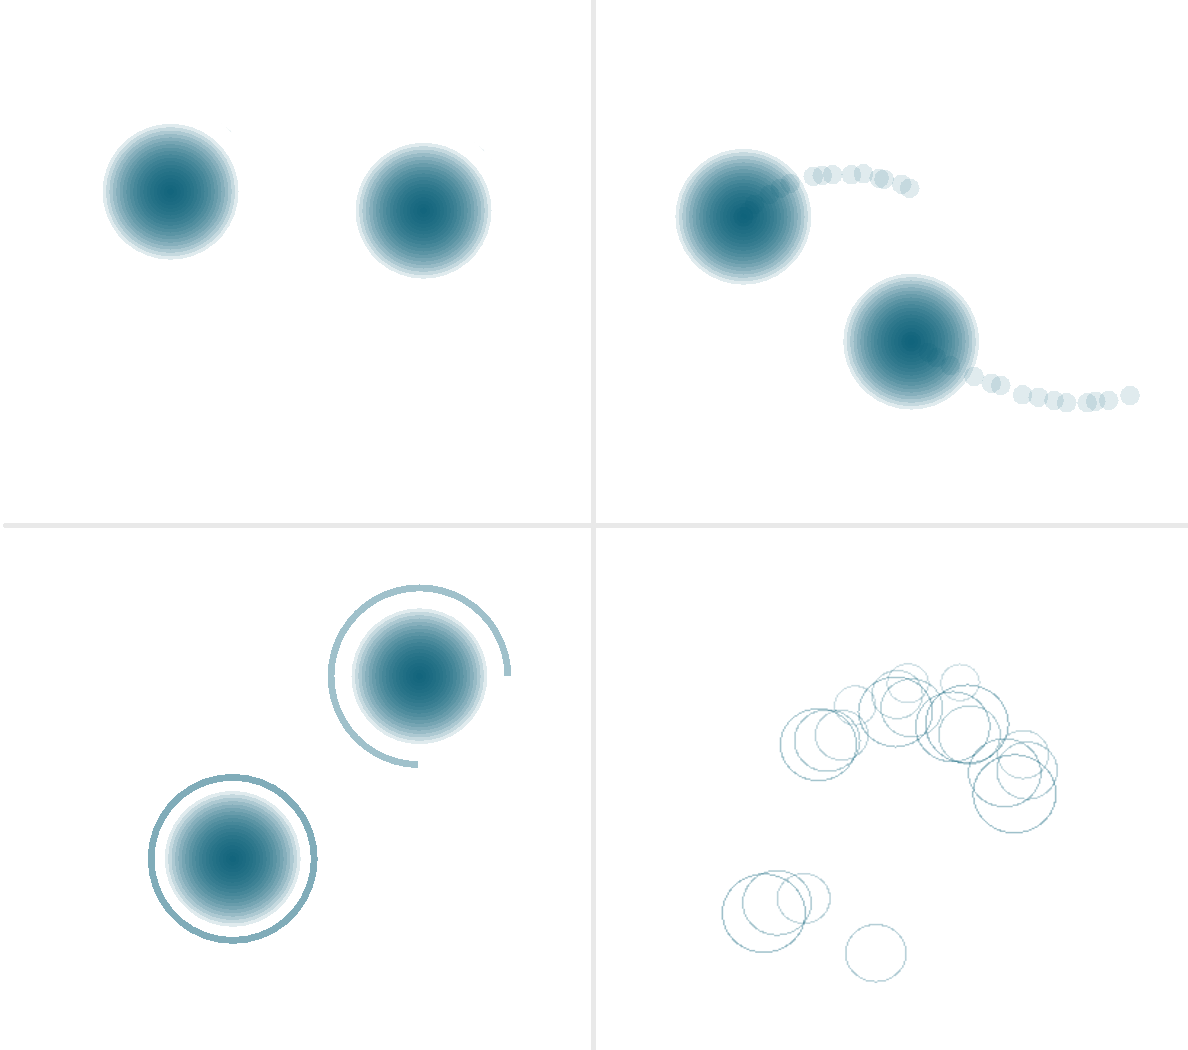
\includegraphics[width=\columnwidth]{feedback.png}
	 \caption[Visual Feedback]{Clockwise from top left: short touches, transitions,
	 unrecognized points, long touches.}
	 \label{figure:feedback}
	\end{figure}
	% =============== 
 

\subsection{Visual Feedback}
When using the keyboard, the mouse and other hardware peripherals, actions are
rewarded with some type of haptic feedback, for example we know when a key on a 
keyboard is pressed of depressed. This behaviour allows people to be more keenly 
aware of the system's current state. This is not true with touch interfaces,
with touch and sensing technology, it is possible for touch points to become lost during a gesture. 
This is due to the users unconsciously lifting their fingers. When this happens people 
can get confused because they may be not be aware that their touch points are lost 
since their fingers are still contacting the surface, there is no feedback
system to alert the user that the actual touch point had disappeared. To accommodate the lack of
physical responses, we implemented our own visual feedback. We created
four different types of visual cues, which we summarize below and can be seen in
Figure \ref{figure:feedback}. 

\begin{itemize}[noitemsep]
  \item Short Touch Point: Whenever a touch point is registered, we render a gradient
  circle at the XY screen coordinate as detected by the sensor. The
  radius of the circle is slightly larger than the average fingertip such that
  is is always visible (about 15 pixels on our display). The position of
  the circle is updated to synchronize with sensor updates, and is removed
  when the touch point is rescinded. This visual cue provides viewers immediate
  feedback of the active touch points.

  \item Long Touch Point: A long touch point has the same basic visual cue as a short touch point.
  A long touch starts off as a short touch point, a ticking timer running in the
  background determines when the short touch transitions into a long touch. We
  visualize this timing sequence as an arc outside of the circle, which expands
  with an increasing central angle and opacity that are mapped to the amount of
  time elapsed. A long touch gesture is achieved once the arc has travelled
  the entire circumference, becomes a ring and locks down. Any interruption
  during the transition phase will remove the animation, the gesture will return
  back to a normal touch point.

  \item Trails: The system keeps track of previous updates for all points.
  We visualize up to the last 10 most recent updates as breadcrumb trails. 
  The trails serve as a reminder of the type of high level gesture that is being
  performed. Furthermore it serves as an additional visual cue to identify the
  current touch point location. The trail points are rendered as smaller
  versions of touch points.
   
  \item Unrecognized Points: These visual cues are used to denote points that were 
  rejected by our evaluating heuristics. This
  cue gives the viewers some sense of the hardware capabilities and
  deficiencies. We think this is useful as a learning device since viewers are able
  to see where they may inadvertently cause unwanted touch points and use this
  experience to adjust how they operate their gestures next time they interact
  with the display. We visualize this as unfilled circles that decrease in
  opacity and radius with time, they are removed from the system when the radius
  reaches zero.
\end{itemize}
 
An additional visual feedback was created to visualize processing time. Due the 
size of dataset, the system may incur a slight delay between re-evaluation of the
visualization. We draw a small clock icon at the position where the last action 
was performed to indicate the system is processing, the clock fades into the 
background once the data processing is completed. 





 
%%%%%%%%%%%%%%%%%%%%%%%%%%%%%%%%%%%%%%%%%%%%%%%%%%%%%%%%%%%%%%%%%%%%%%%%%%%%%%%%
% This chapter describes the analytics tools and views
%
% - Should rewrite comparison section, see pacivicVIS paper
%%%%%%%%%%%%%%%%%%%%%%%%%%%%%%%%%%%%%%%%%%%%%%%%%%%%%%%%%%%%%%%%%%%%%%%%%%%%%%%
\chapter{Enabling Analysis}
A comprehensive analytic system requires a variety of ways to manipulate and
looking at data. In this section we describe solutions for trend detection,
making comparisons and high level overview.
 

\section{Heatmap Perspective}
The heatmap widget has generic support for visualizing a time series data. It 
allows different time series to be interchanged within the heatmap itself, showing 
different perspectives. This was done to support the different types of
analytical tasks discussed in Chapter 3. These tasks, such as
finding seasonal trends of a component and finding the worst performing
component, are quite different, requiring a localized view showing how a
single component performed over time, and the other requires a very high level
view designed to draw out outliers.

    % === Figure === 
	\begin{figure} 
	 \centering  
	 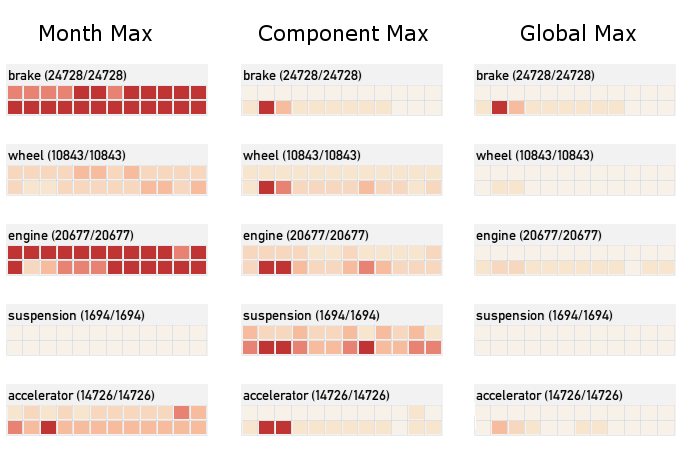
\includegraphics[width=\columnwidth]{heatmap_2.png}
	 %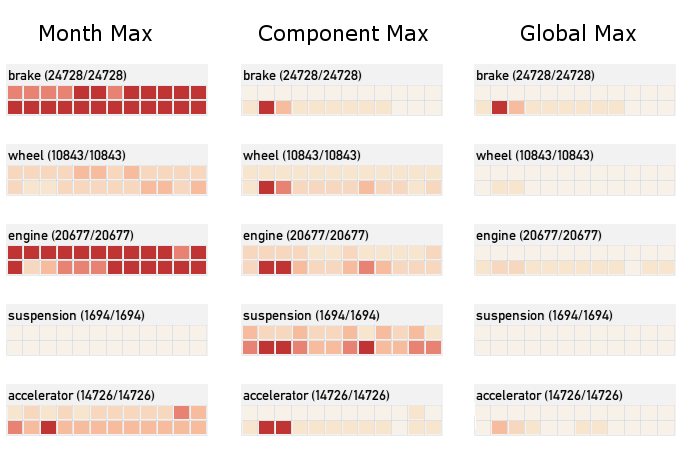
\includegraphics[scale=1.0]{heatmap_2.png}
	 \caption[Heatmap Perspectives]{The different heatmap perspectives. Left
	 displays the monthly perspective, centre displays the component perspective, and right displays the
	 global perspective}
	 \label{figure:heatmap}
	\end{figure}
	% ==============


Our visualization provides several different perspective views as shown in
Figure \ref{figure:heatmap}, all based on the occurrence score. The score of
each entity of each month is transformed by a divisor, which determines the
type of semantic we want to show. The available heatmap perspectives are listed below:

\begin{itemize} [noitemsep]
  \item Month-Max: A monthly perspective where the score of each month is 
  divided by the maximum score for that month amongst all components in the selected time.
  
  \item Component-Max: An entity-level perspective where the score of
  each month is divided by the maximum month score of the entity over the
  selected time. This is the default perspective in the system.
  
  \item Global-Max: A global perspective where the month score is divided by the
  maximum overall monthly score.
\end{itemize}
 
Here we illustrate how the perspective scoring works with an example of a time
over a period of three months: Suppose there are two entities, engine and brakes
and their occurrences scores over the three months are (1, 10, 100) and (10, 15,
20) respectively. In Table \ref{table:perspective} we show the entities' month
score under each perspective.

The monthly perspective draws out the
highest scored entity of each month, thus they are 10, 15 and 100 over the 3
months shown. Component view is localized for each entity, thus it is 100 for
engine entity and 20 for the brake entity over the 3 months. Finally global
perspective uses global maximum as the divisor, which is found in the engine
entity in the third month.
 
    % === Table ===
    \begin{table}[h]
	%\begin{tabular}{| l | lll | lll | lll | lll | 
	\begin{tabular}{| l | lll | lll | lll | 
	      } 
	   % Column Heading
	   \hline
	   %& \multicolumn{3}{|c|}{Score} 
	   & \multicolumn{3}{|c|}{Month Max} 
	   & \multicolumn{3}{|c|}{Component Max} 
	   & \multicolumn{3}{|c|}{Global Max} \\
	   
	   % Data 
	   \hline
	   Engine & %1 & 10 & 100 &       % Original
	            1/10 & 10/15 & 100/100 &      % Month
	            1/100 & 10/100 & 100/100 &    % Component
	            1/100 & 10/100 & 100/100 \\   % Global
	            
	   Brake &  %10 & 15 & 20  &      % Original
	            10/10 & 15/15 & 20/100 &      % Month
	            10/20 & 15/20 & 20/20  &      % Component
	            10/100 & 15/100 & 20/100 \\   % Global
	   \hline
	\end{tabular} 
	\caption{Sample perspective based scores} 
	\label{table:perspective}
	\end{table}
	% ============
  
Each of the perspectives above answers different questions and has its own
advantages and disadvantages. The month-max perspective allows people to compare 
component-to-component by month, but comparison against adjacent cells are 
meaningless because each cell uses a different base value. The component-max 
perspective is the opposite, it allows us to see trends with a single entity, 
but it does not allow comparison across components. Lastly, the global-max 
perspective is good at showing the outliers and supports both month-to-month 
and component-to-component comparisons, but it is difficult to see overall
trends because the outliers, if any, will dominate and push all non-outliers
into the same scoring bin.

To put the different perspectives in better context, we compile a list of sample 
questions that can be answered with these different perspective views:
\begin{itemize} [noitemsep]
  \item Month-Max: In month X, which vehicle component had the most complaints?
  \item Component-Max: Are there more braking problems in the summer months or
  the winter months? Are the number of complaints for wheels increasing or
  decreasing?
  \item Global-Max: What are the most unreliable vehicle components?
\end{itemize}

Going back to Figure \ref{figure:heatmap} as an example, one can make some
interesting observations. From the component view in the centre, a person can
see that there are two distinct outliers in the second and third months of the
second year, in particular, one can see the scores getting lower, then there is
a resurgence around July and August in the second year. Switching to the month-maxa
perspective, one can observe that during the two year period, the most
significant components seem to alternate between the brake and engine component,
with the sole exception of accelerator appearing in a single month. Lastly, the
global perspective yields three outliers, February and March from the brake entity
and February from accelerator entity. However, note the rest of the cells are
pushed into the lower brackets and not possible to detect any other trends.
 
The heatmap viewing perspective is at a global scope, thus a change in
perspective will affect all visible heatmaps. This keeps the interface
consistent and avoids viewers from switching to different modalities when they
shift their attention from one heatmap to another. The view switching mechanism
is realized as a drop-down control sitting atop the hierarchy widgets and shows
the currently selected viewing mode.



\section{Comparison}
Comparison mode allows people to compare entity occurrences across
two different subsets of the data. To select data to compare, we provide
two sets of filter widgets which can be used to specify manufacturer,
make, model and model year. Each set of filters specifies a query,
which we will call Q1 and Q2, and each query is assigned a colour,
which is used in the visualization. For example, we can compare
Honda Civic (Q1) to Toyota Corolla (Q2), or we can compare Ford
Focus (Q1) against all other Ford vehicles (Q2), by not fully specifying Q2.

Two separate measures are used to render the comparison view.
The \emph{contribution sum} is the aggregated component score from the two
query sets: it reflects the overall importance of the component by emphasizing
the most frequently occurring components matching Q1 and
Q2. The \emph{percentage difference} describes the relative frequencies of a
component, whether it occurs more frequently under Q1 or Q2 relative
to the total contributions from Q1 and Q2 respectively. The percentage
score is calculated as the component score divided by the total
contribution. Then the percentage difference follows as percentage
score Q1 minus percentage score Q2, with the sign and magnitude indicating
which query set has the stronger presence of that component.

We made the decision to use percentage-based comparisons because it
enables the comparison of query results of different sizes. For example, we can compare
a large manufacturer against a small manufacturer, even though we would expect the large 
manufacturer to have a greater number of complaint reports.
These scores are used to render the \threed view. Using the percentage
difference, the colour of the outline of a component indicates which
query set has the higher rate of complaints, and the opacity of the outline
indicates the strength of the difference. Using the contribution
sum, the standard hue and opacity encoding is used to indicate the
sum of the two query sets, giving an impression of the overall importance
of that component. Thus, a highly problematic component from
both queries will have a strong presence overall but with a faint outline,
while a lopsided but infrequently mentioned component will have
strong outline but barely visible interior colour.


    % === Figure ===
	\begin{figure}
	 \centering  
	 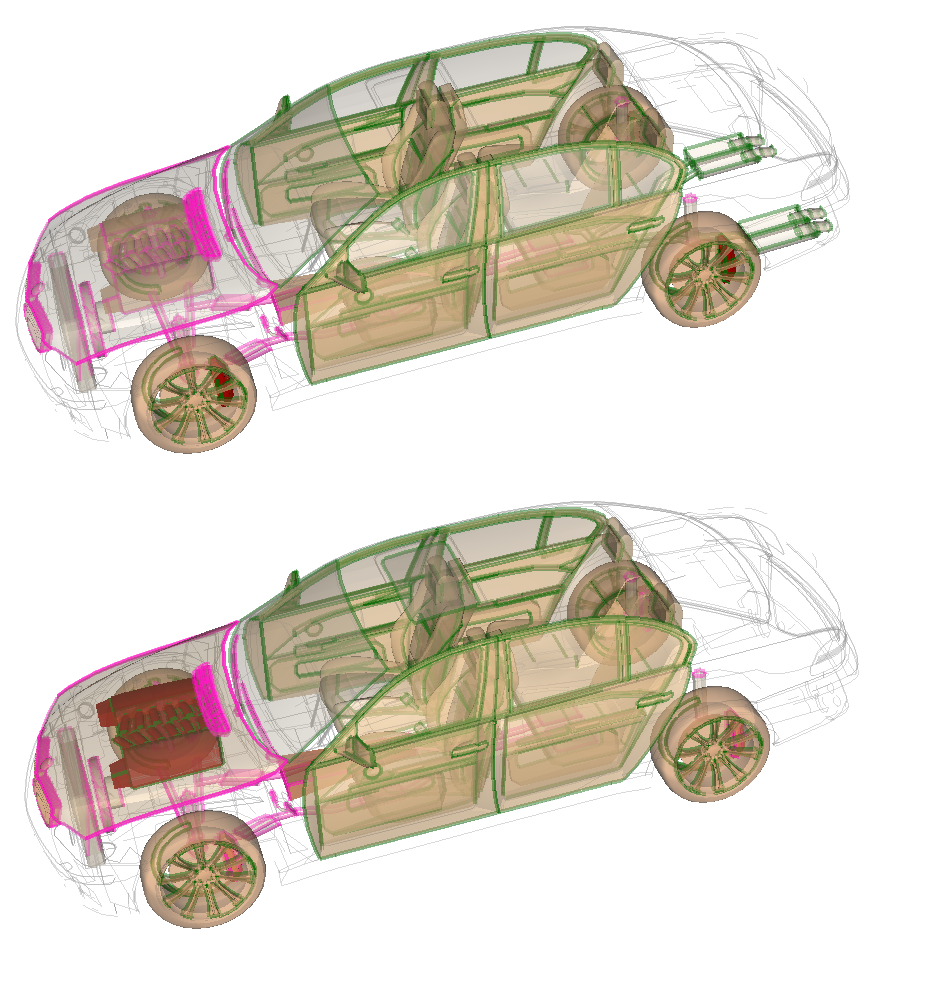
\includegraphics[width=\columnwidth]{comparison_3.png}
	 \caption[Comparison View]{Top: Vehicle A (pink) versus vehicle B (green), the
	 brake appears to be the dominant issue and B has the higher rate of complaints. Bottom:
	 Vehicle A (pink) versus vehicle C (green), the engine is the dominant issue
	 and B has higher rate of complaints.}
	 \label{figure:comparison}
	\end{figure}
	% ============== 
 
%As an example, see Figure \ref{figure:comparison}, where we compared Plymouth
%against both the Jeep and Chrysler. At a glance most parts remain the same
%with the exception of two outliers, Jeep appear to have a higher failure rate
%than Plymouth, and Dodge has a higher failure rate in brakes component. The
%overview could suggest that Plymouth is more reliable than both vehicles.

As an example, see Figure \ref{figure:comparison}. Vehicle A (pink) is compared
first against vehicle B at the top and vehicle C at the bottom. We can observed
that vehicle A has more complaints about the hood than both B and C. We can also
infer that B has serious problems with brakes and C has serious problems with
engine.
 
By default, comparison mode is turned off. It is activated when the viewer
switches the second hierarchy widgets from the ``None'' position to a valid
selection. Subsequent query modifications are carried out in comparison mode
until the selection is turned to ``None'' again.

%One limitation with this approach is our current usage of the total
%contributions to calculate the percentage scores. Our total contribution is in
%relations to the number of documents in the corpus, which may not be
%the best indication of the overall contribution.

 
 
 
\section{Aggregation}
By default, the system treats each object individually rather than object
groups. For example ``seatbelt'', ``backrest'' and ``seat'' are all processed
separately, even though they are logically under the group ``seat.'' This
setting allows people to isolate and identify low-level problems accurately. There
are times, however, when this level of information is unnecessarily detailed and
a higher level of abstraction is desirable.

    % === Figure === 
	\begin{figure}
	 \centering  
	 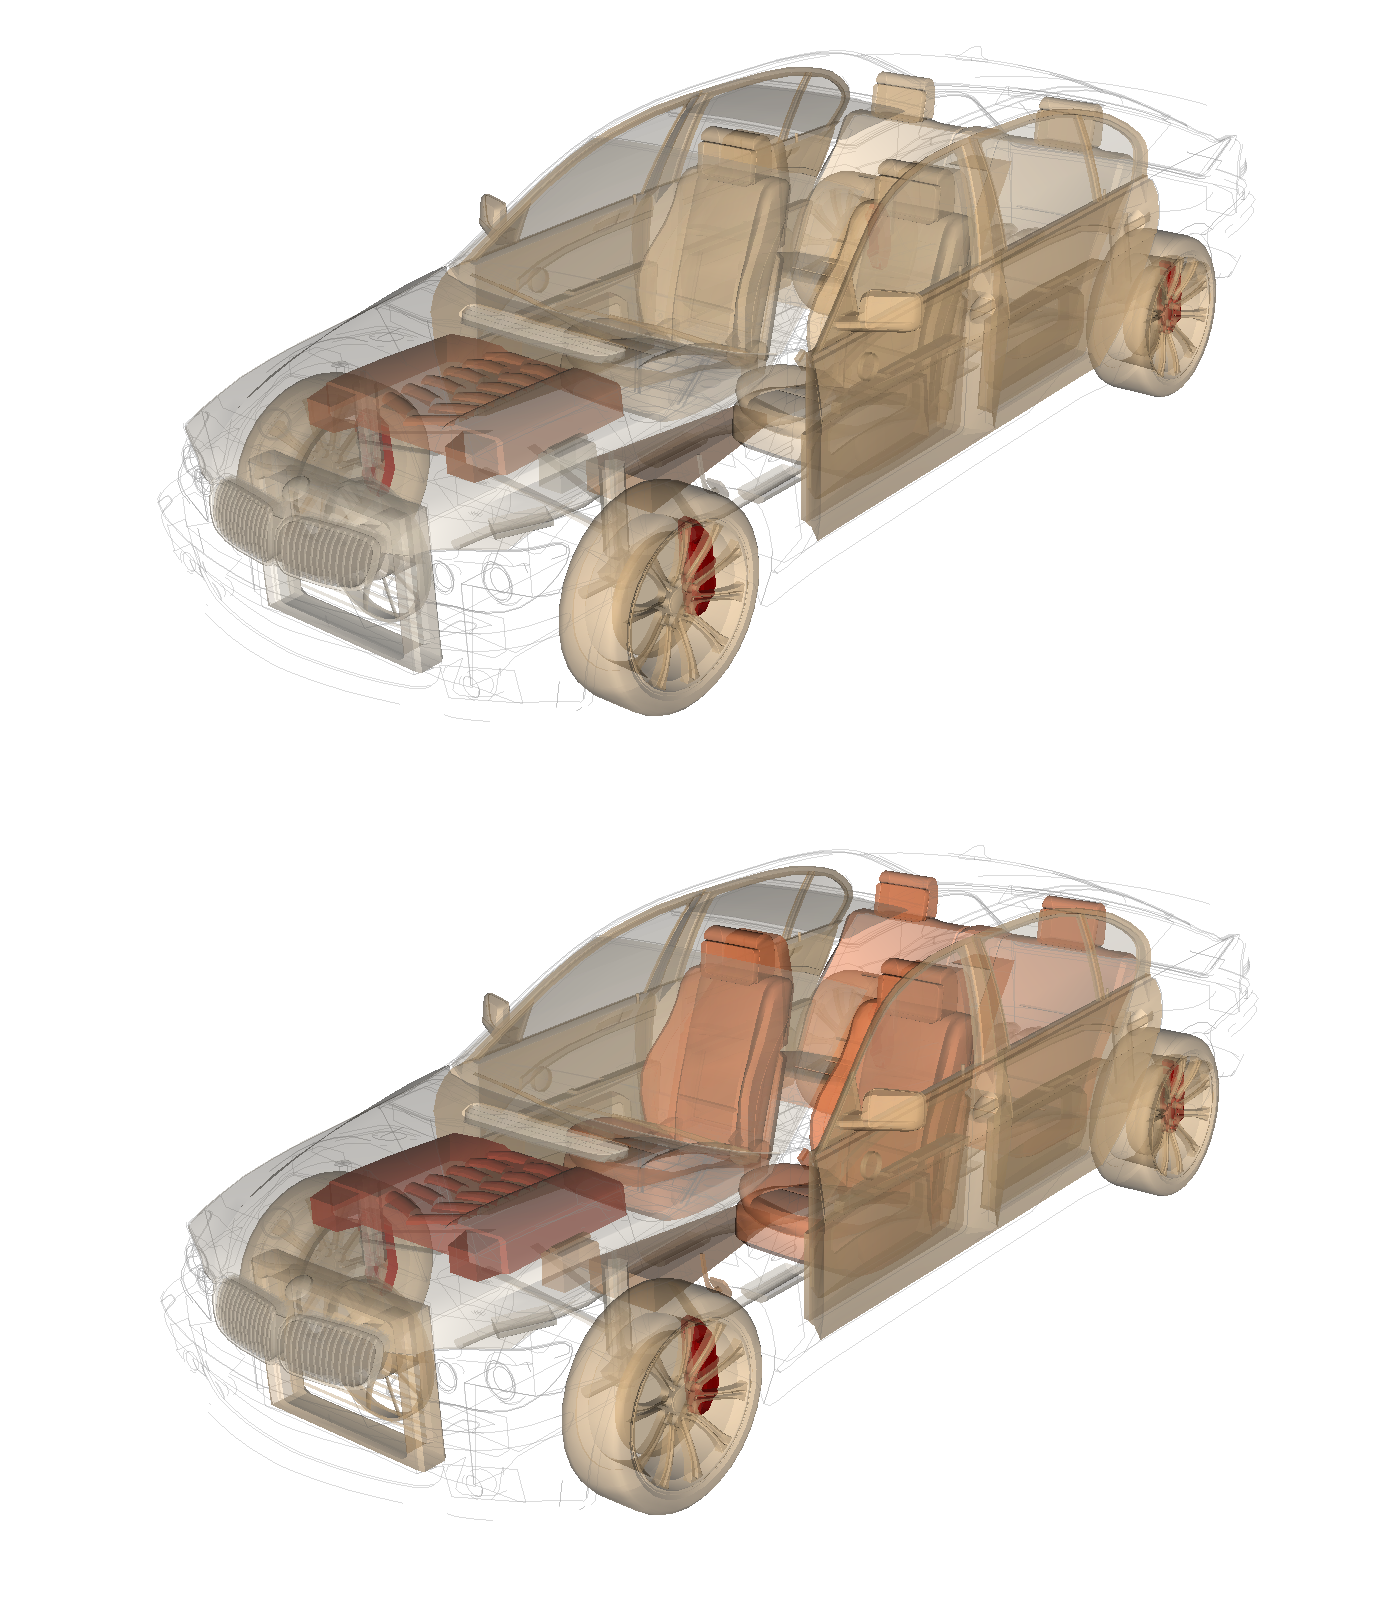
\includegraphics[width=\columnwidth]{aggregation2.png}
	 \caption[Aggregation View]{Top: Aggregation mode disabled. Bottom: Aggregation
	 mode enabled, note that the seat now appears more prominent in the visualization.}
	 \label{figure:aggregation}
	\end{figure}
	% ==============
	
Aggregation mode mimics the type of high level rating system found on consumers
review websites. When aggregation mode is enabled, individual objects, and their
scores are aggregated up to the first level entities in the keyword hierarchy. In our specific case, the 
first level are the major sub-systems in a vehicle. Aggregated components
responds to interaction events as a single group, thus, selecting the
``seatbelt'' will select the entire ``seat'' subsystem.

 
Figure \ref{figure:aggregation} shows a before and after illustration of using
aggregation mode. A default rendering is shown in the top portion, one can
only observe that brakes is the most severe out of all components. The bottom
shows the aggregated view, one can observe that on a higher level, the seat
subsystem is quite problematic.
 
Aggregation mode is enabled/disabled by a toggle switch located at the top
portion of the display interface. Aggregation mode works in
conjunction with comparison mode, allowing people to make comparison of major
systems.

%%%%%%%%%%%%%%%%%%%%%%%%%%%%%%%%%%%%%%%%%%%%%%%%%%%%%%%%%%%%%%%%%%%%%%%%%%%%%%%%
% Implementation and algorithm details
%
%%%%%%%%%%%%%%%%%%%%%%%%%%%%%%%%%%%%%%%%%%%%%%%%%%%%%%%%%%%%%%%%%%%%%%%%%%%%%%%%


\chapter{Implementation}
In this chapter we discuss the design of the visualization system in brief. We
then look at some of the non-trivial issues that were encountered during the
implementation phase, what are their impact on the visualization as a whole and
our solutions.
 

%%%%%%%%%%%%%%%%%%%%%%%%%%%%%%%%%%%%%%%%%%%%%%%%%%%%%%%%%%%%%%%%%%%%%%%%%%%%%%%
\section{Environment and Architecture}
The implementation of this prototype is done in the Java programming language.
Graphics are rendered through Java for OpenGL graphics library. MySQL
database is used to host the raw text and document tags. Our graphics hardware
is a NVIDIA Quadro FX video card, and we were able to achieve a frame rate
between 15 to 30 FPS. The prototype is designed to run on 1680x1050 screen
resolution.

    % === Figure === 
	\begin{figure}
	 \centering  
	 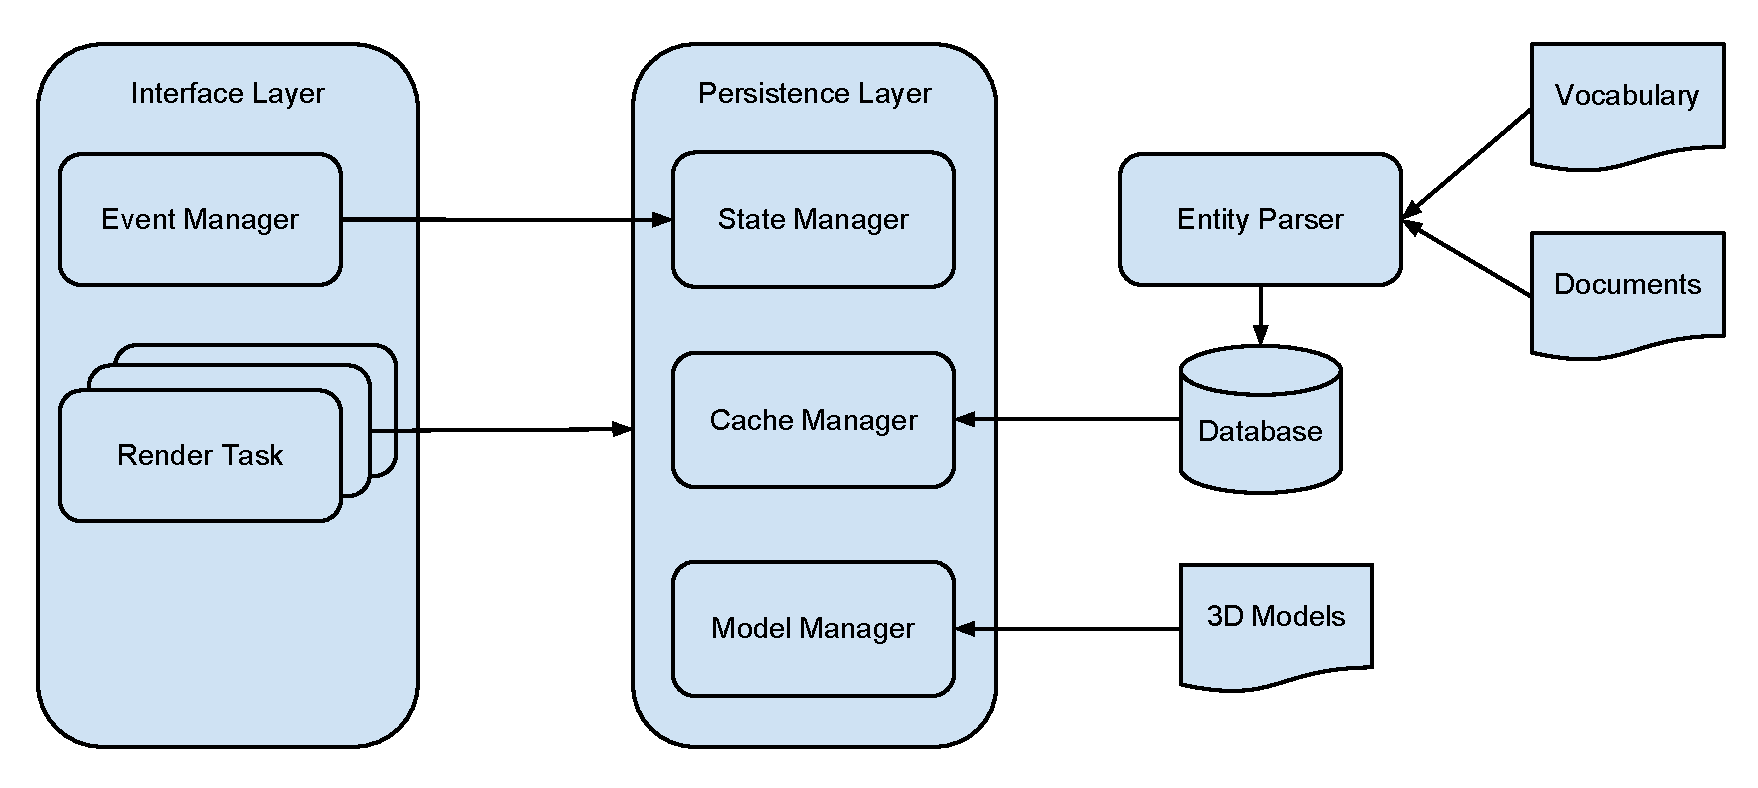
\includegraphics[width=\columnwidth]{Architecture.pdf}  
	 \caption{High level system architecture.}
	 \label{figure:arch}
	\end{figure}
	% ==============

The application can be decomposed into two subsystems: a parser system for
generating entity scores and a visualization system. A  high level overview of
the system architecture is shown in Figure \ref{figure:arch}. The
entity parser consumes two inputs, the keyword hierarchy and the document texts, it
will then compute occurrence and co-occurrence scores and write the results to
the database, the parsing details are covered in Chapter 4. 
 
The visualization system implementation uses a standard two-tier design: A
persistence layer and an interface layer. The persistence layer is in charge of
database transactions, cached resources and system states. The interface layer
takes care of the rendering and any user triggered events. The visualization is
state-driven and the current state is stored in the persistent layer. The
reason for a state machine model is to allow us to programmatically  alter the
visualization, and allow the system to be deployed to different platforms
without major changes.

The major modules of our system, as well as their functionalities are listed below: 
\begin{itemize}[noitemsep]
  \item Render Task: Each rendering task is responsible for rendering a
  functional part of the interface. We have 4 primary rendering tasks: \threed
  visualization, filters, lens, and visual feedback. All rendering tasks poll
  the persistence layer at the beginning of their draw-loop to check if there
  are any updates.
  
  \item State Manager: State Manager keeps track of all states used to calculate
  the current visualization, as well as the states of all interactive elements.
  
  \item Model Manager: The model manager stores the \threed model geometries, it
  allows access to \threed information at various levels: models, components,
  polygons and finally vertices.
  
  \item Cache Manager: Cache Manager is responsible for handling all actions
  that impact the occurrence and co-occurrence scores, as well as any database
  queries.
  
  \item Event Manager: Event Manager listens to user interaction events, it
  communicate changes to the State Manager. All the hardware specific tunings
  reside in Event Manager.
\end{itemize}




%%%%%%%%%%%%%%%%%%%%%%%%%%%%%%%%%%%%%%%%%%%%%%%%%%%%%%%%%%%%%%%%%%%%%%%%%%%%%%%
\section{Algorithms}
During the development of the software prototype, we have encountered several
non-trivial problems. While these issues are not a part of our visualization 
design, they nonetheless impact overall user experiences via the degradation 
of aesthetic and usability of the system. In this section we discuss these 
problems and our proposed solutions.

\subsection{Order Independent Transparency}
Chapter 5 mentioned briefly that rendering translucent geometries in \threed
space can create artifacts, here we will describe this in greater detail and outline
our work-around solution. There are two options in the graphics API that
controls transparency effects:
\begin{itemize} [noitemsep]
  \item Enable Blending: This option allows foreground objects to blend with
  background objects.
  \item Disable Depth Testing: This option renders all geometries regardless of
  depth and overlaps.
\end{itemize}

    % === Figure === 
	\begin{figure}
	 \centering  
	 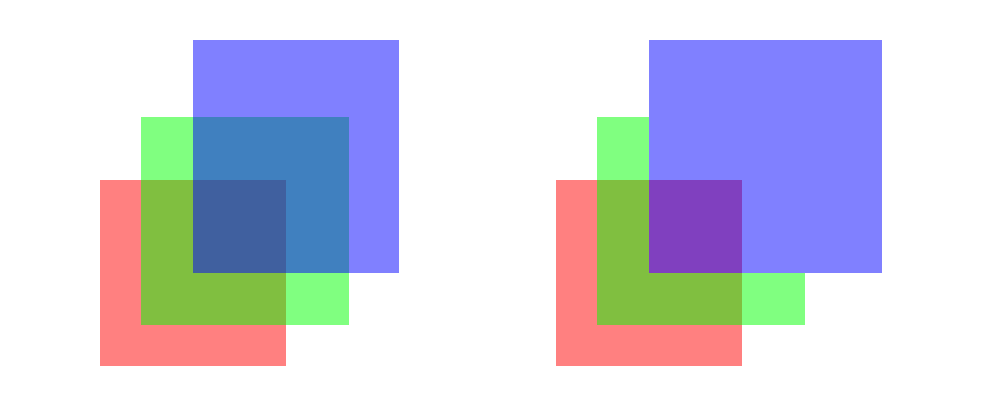
\includegraphics[width=\columnwidth]{oit_example.png} 
	 \caption[Order Independent Transparency]{The left image is rendered in
	 correct back-to-front order. The right image is out-of-order, the green
	 square does not properly blend into the blue square.}
	 \label{figure:oit}
	\end{figure}
    % =============

Geometries are typically not sent to the hardware in sorted order, so they are
neither front-to-back nor back-to-front. Hardware supported depth buffer
resolves the out-of-order polygons by selecting the fragment closest
to the eye position. With transparent effect in place, fragments are blended
together rather than going through the selection process. Where the problem
arises is that alpha-blending is not commutative, for example: red+green+blue
is not equivalent to red+blue+green. The effects of out of order blending versus
in order blending is seen in Figure \ref{figure:oit}.

The major problem of out-of-order blending is that objects that are supposed to
be behind can appear to be in front, making it difficult for the viewers to
judge an object�s depth correctly. In the visualization, this is not only
distracting, but can mislead viewers to select incorrect entity components.


Naively we can use either sort the geometries or use space partitions to force
geometric objects into depth order, However, these naive solutions tend to have
very expensive computation, and are view dependent which results in
re-computation whenever the viewing perspective changes. There are also
pathological cases where polygons intersect each other, which cannot be solved
with partitioning or sorting alone.

Alternative blending algorithm exist that looks at minimizing the effects of
order-dependent terms in blending equations, but there is a threshold on the
amount of transparency that can be applied~\cite{Meshkin2007, Bavoil2008}.
Other works use hardware features to allocate a buffer to emulate
sorting operations~\cite{Myers2007, Bavoil2008, Yang2010}, these algorithms
produce more accurate results, albeit bounded by hardware constraints or the complexity of
the scene itself.  

In this prototype, we use an implementation of dual-depth-peeling
\cite{Bavoil2008}, which ``peels'' the \threed scene apart layer by layer
into textures, before recomposing these texture into a final texture in depth
order. The implication of this peeling effect is that it effectively changes the
rendering process from single to multiple passes, and that performance depends
on the depth complexity of the scene. This method yield accurate and
eye-pleasing results, while more performance friendly methods exists, we decided
that this was the most reasonable approach because the required features are
available on most hardware at the time of implementation.
  


% \subsection{Effects}
% Here we briefly discuss our usage of graphical effects. OIT rendering, as
% described above, is used to ensure correct depth cues, it is possible to achieve
% different look and feel by passing different lighting equations to the shader
% programs. Halo effect is done by calculating silhouettes in \twod space of the
% active entities, we then subtract the geometric shape from the silhouette, and
% perform a smoothing step to blur out sharp features on the outline. The ghostly
% outline effect is done by calculating ridge and silhouette edges of adjacency
% structures in the mesh, as outlined in Hermosilla's GPU implementation
% \cite{Hermosilla2009}. Finally the lens effect is achieved through adding and
% subtracting of textures, the full scenes with lens semantic is rendering into a
% texture, we alter the non-lens area to be completely transparent and superimpose
% the remainder onto the existing scene.

 

\subsection{Cache and Stabilization}
Because the size of the dataset used to render the visualization can vary
greatly, database query performance tends to vary as well. To compound the
problem, most queries in the system are aggregation based queries and create
additional performance overhead. Overall database execution time can vary from a
few milliseconds to several seconds, we found this to be unacceptable because
it degrades user experiences.

Here we introduce an intermediate in-memory cache to store the aggregated scores
of each entity. The cache is created at system initialization,
then queries are executed against the cache rather than the database.
The cache organization is specific to this dataset, however the idea itself is
generalizable.

Cache is realized as a hierarchy of lookup tables. It is modelled based on
the time and hierarchy filters and how we perceive people use the visualization.
The cache levels are, from most general to most specific: time period, entity,
manufacturer, make, model and model year. 

Each node in the cache hierarchy contains three things, a reference to all its
direct children nodes, an aggregated score of all its children, and a reference
to the documents that match the node which are used to calculate co-occurrence. For
example, a node corresponding to (July 2010, engine) will have the following:
\begin{itemize}[noitemsep]
  \item An aggregated score total that indicate the number of occurrence of
  engine in documents relating to incidents during July 2010
  
  \item A listing of unique document IDs that match the above criteria
  
  \item References to children nodes (manufacturers) that matches the above criteria
\end{itemize}

The overview visualization is then constructed by iterating over the desired
time periods. We then apply the hierarchy filters to find the correct cache
nodes for each entity parts, and finally sum up the node's entity scores across the
time periods. Because cache table lookup is close to constant time, our queries
result in a much more stable performance compared against database queries. On
average we found the cache queries take about 100 to 200 milliseconds to
execute, which we found to be acceptable.




%Due to the size of our data and the diverse variations of queries on the
% database, we have encountered situations where our database does not produce a stable 
%performance. We have found with SQL queries alone our query results come back 
%between several milliseconds to a few seconds. A major part of this delay is due 
%to the nature of the queries, which are mostly aggregates that result in sorting 
%operations. We found this to be unacceptable, because it defies people�s 
%expectation of instantaneous reaction from the system.

% To create a better user experience in-line with user expectations, we created
% a hierarchical lookup table that partially caches the aggregated query results. 
% Each level corresponds to a unique filtering criteria based on our dataset, for 
% this prototype, we have from highest level to lowest level : time, entity, 
% manufacturer, make, model and year. The hierarchy order models the type of 
% successive query refinement we expect of typical interactions. Each entry, in any 
% level, corresponds to the aggregated query up to that specific point. Each entry 
% contains a value that is the aggregated count of the documents, as well as a 
% reference to a list of its children, if applicable. For example: (``2000'',
% ``engine'', ``Toyota'') will yield the query results of all Toyota vehicle
% complaints that had engine problems in the year 2000. To create ranged query, for example 2000 to 2005, we 
% issue the same query with different time parameters and sum up the results. More 
% complex queries such as aggregation and co-occurrences, are done in similar manner, 
% but with different lookup tables. In practice, we found this to be a middle of the 
% road approach. Comparing to raw database queries, it performs slower than best case 
% but much faster than the worst case scenarios, most important of all, we have 
% consistent performance at around 100 to 200 millisecond, which we found to be 
% acceptable for interactive use.
% 
% The table is created at when system starts, we iterate through the database
% tables once, creating the hierarchy structure and increment the counts as we go. As a last 
% optimization step, we have attempted to serialize out the query tables to disk, 
% so they can be de-serialized on system startup without having to iterate the
% database tables. However, without a customized data container, this in practice turned out 
% to be slower than database lookups and was abandoned.


\subsection{Multi-Touch Heuristics}
Touch sensors have a few drawbacks; there are inherent noises that come from
performing gestures, in addition, our inability to hold our hands perfectly
still accentuate this issue by creating jitters. In our particular use case, the
upright display makes certain gestures difficult, for example, in an informal
evaluation of the display we found that certain curvatures introduced a
lot of noises because the knuckles of other fingers are sensed as
false-positives as result of drifting too close to the screen itself.

These noises degrades user experiences, as they trigger unexpected events within
the system. We introduced a set of software heuristics as an intermediate step
between when the points are sensed and when they are executed. In general, these
heuristics remove unintended touches and prevent jittery animations that
result from minute movements. While these are designed specifically to deal with
our hardware issues, we believe rules are general enough that they can be
adopted to other touch sensors. 

\begin{itemize} [noitemsep]
  \item \textbf{Real Update:} The muscle deformation when pressed against the
  display, paired with inability to keep still postures result in
  sensor registering jittery updates. This is undesirable because it induces a
  shaking effect, and often time unnecessary because the updates are minute.
  To compensate, the system only accept an update if it is at least
  X number of pixels away from the previous updated point.
  
  \item \textbf{Coincidental Points:} When a touch is initialized on the touch
  surface, there is a possibility that more than one touch point will be
  registered. This is similar to the case we presented above. To reduce this scenario from
  occurring, we store the XY-coordinate and the time that the touch point is
  created. If a touch point is created too close to any other touch point within a time
  threshold X, that point is rejected.
  
  \item \textbf{Movement Buffer:} When a gesture is in transition, there are
  cases where other parts of the hand will inadvertently cause false-positives.
  We try to neutralize these occurrences by introducing buffer zones around touch
  points that are in motion. New touch points cannot be created 
  if they fall within X pixels away from a point that is in transition.
  
  \item \textbf{Reinforce Intention:} This heuristic deals with reducing jitters
  on the initial touch. This can be seen as a special case of the Real Update
  heuristic, but while Real Update toss away extremely small update in general,
  the first update can be quite large, probably due to the act of pressing the
  finger against the display. We made it such that the first update must be at
  least X pixels distance in magnitude. This heuristic is not applicable to
  lens widget nor document widget because we want them to be immediately
  responsive. 
  
  \item \textbf{Dead Zones:} In some cases, the act of lifting up
  a finger to disengage a gesture will trigger a new touch point. This makes
  selection problematic, as selected entities will be deselected right away. To
  resolve this issue the system impose dead zones. When a touch is removed, the
  area around it will become unavailable for a small amount of time, during
  which all new touch points are ignored.
  
\end{itemize}


 
%%%%%%%%%%%%%%%%%%%%%%%%%%%%%%%%%%%%%%%%%%%%%%%%%%%%%%%%%%%%%%%%%%%%%%%%%%%%%%%%
% Scenarios and Evaluation
% - Find a nice way to mention the scenario and how the visualization works
% - Probably want to divide up the discussion section for the study and expand
%   it a bit more.
% - Scenario ideas
%      > Spatial with lens 
%      > Toyota recall analysis 
%      > Comparison during car purchase ???
%%%%%%%%%%%%%%%%%%%%%%%%%%%%%%%%%%%%%%%%%%%%%%%%%%%%%%%%%%%%%%%%%%%%%%%%%%%%%%%%

\chapter{Scenarios and Evaluation}
In this chapter, we present several scenarios to show the possible uses cases
for our visualization. Following that, in the second section we present a
qualitative evaluation study of our system, discuss the study results and our
observations.

%%%%%%%%%%%%%%%%%%%%%%%%%%%%%%%%%%%%%%%%%%%%%%%%%%%%%%%%%%%%%%%%%%%%%%%%%%%%%%%%
\section{Scenarios}
We present three different scenarios to show how different facets of the
visualization can be used to analyze data and facilitate decision making tasks.
The first two are hypothetical scenarios and are used to demonstrate our system
functions: spatial exploration and making comparisons. In the third and last
scenario, we take a look at a real world event and see if the dataset reveals
any interesting facts surrounding the event.

 
\subsection{Spatial Exploration}
This scenario describes how a regular consumer, Larry, may use the 
visualization to research a problem. Larry has about three years of driving 
experience but does not know a lot about cars. Recently, while driving, he 
noticed a rattling sound coming from the passenger side of his vehicle. 
He decides to conduct some research on his own before taking the car back 
to the dealership.

Using the visualization, Larry filters the dataset to focus on his
vehicle model. Since Larry is not sure exactly where the noise came from, 
he uses the lens widget to focus on components near the front-passenger 
region. Using the lens, Larry can see that the suspension component has a
higher number of complaints registered against it than the other components 
in the focused area. Larry then selects the suspension component using 
the heatmap, and toggles the document widget so he can read through the 
actual complaint reports. After a few minutes of reading, Larry notes that
there are at least eight or nine reports that seemed to document similar noise 
issues and point to defective suspension setup. Larry decides that he 
should contact his dealership to have them check it out.

 
\subsection{Vehicle Comparison}
This scenario describes how our visualization may guide purchasing decisions.
Sara just accepted a job offer across town, and is looking to purchase a car 
for her commute. She previously had her mind settled on a used Honda Civic, 
but her friends have been saying good things about Nissan Sentra. With the 
visualization system, Sara uses the comparison function to compare Civic to 
Sentra, she then turns on the aggregation mode function so the visualization 
shows the system level view. 

Sara sees that engine and wheel components are both lightly shaded, which
indicates that neither one had serious issues regarding these sub systems.
However, she notices that there are dark green outlines around several
components, using the lens she identifies them as parts of the transmission subsystem. It seems like Sentra had
a much higher rate of transmission failure than Civic. Selecting the
transmission, Sara reads through several complaint reports, Sara then decides
that her original intuition about Honda Civic is correct.


\subsection{Retrospective Analysis}
In this scenario, we use our system to examine the Toyota recall. The Toyota 
vehicle recall happened between September 2009 to February 2010 and had to
do with defective brakes and accelerators. We are curious to see if there are
any patterns, in terms of leading or lagging indicators in the complaint data.
We set the time sliders to show 2009 and 2010 as seen in Figure \ref{figure:heatmap} 
and use the heatmap widget to observe for patterns.

The first thing we noticed is that the engine, usually one of the highest
occurring components in the complaint reports, no longer dominated
the visualization. Instead, two components pop out: brakes and accelerator.
A closer examination with the lens widget raised more questions.
The heatmaps show that there are two outlier months where a
huge amount of complaints were registered: February 2010 and March
2010, after the recall was announced. Perhaps the widely publicized
event triggered a loss in consumer confidence, which in turn led to an
over-reporting of problems. This is supported by the sharp drop-off
after March 2010.

% \subsection{Finding Causal and Related Issues}
% Curly is an automobile defect investigator, he is in the process of gathering
% information about a possible defect in the 2009 model of sedans. He leverage the
% NHTSA database as a data source for consumer initiated complaint reports. He
% enters the criteria one by one: manufacturer, model, make and the date range he
% wants to search for. After reviewing several dozen reports with brake issues he
% notices that there seem to be a trend emerging: over 50 percent of the reports
% read so far also mentions problems with the accelerator pedal. Thinking that
% there may be a connection between these two components Curly decides that he
% should widen his search criteria to include both accelerator and brakes.
% 
% Our system suggest causal relations by explicitly highlighting the related
% entities in text documents. Rather than having to account for related terms in
% his head, Curly can select the brake component in the visualization, which will
% high light all co-occurring entities, include the accelerator. A visual scan
% will reveal the high occurring, which Curly can select, and use the document
% panel to read the detailed complaint descriptions.


%%%%%%%%%%%%%%%%%%%%%%%%%%%%%%%%%%%%%%%%%%%%%%%%%%%%%%%%%%%%%%%%%%%%%%%%%%%%%%%%
\section{Evaluation}
We conducted an evaluation to see how the visualization is perceived and how
people perform analytical tasks. In order to create a realistic scenario, we
leveraged the vehicle complaint dataset. The study is framed around the idea of
analysing safety and reliability concerns. Our evaluation is based on how
participants interpret the visualization and  whether their decisions are
derived based on what the visualization is showing them. We also look at the process
participants go through to complete more open-ended tasks.

%Participants were evaluated on their
%interpretation of the visualization, as well as the process they go through to 
%complete complex scenarios. 

We have considered performance measures, in particular, against existing applications
that allow people to search and browse NHTSA dataset. However, as the application
interfaces are vastly different than ours, we did not believe such comparison would
be fair. Also, the tasks would be severely constrained to be possible on both
interfaces that they may not yield any meaningful results.

%nor would it yield any meaningful results.

%Our hypothesis states that when it comes to visualizing data involving physical
%objects, people may be able to communicate and gain better insights if we
%present the visualization to match real world entities. We take the first steps
%in evaluating our hypothesis by studying how people respond to our \threed
%interface and if they can use our visualization to solve analytical tasks. Our
%primary concerns are not whether the visualization is more efficient than
%conventional interfaces, rather, we focus on the type of questions that can be
%answered by our software as well as the user-experiences of using our prototype.


\subsection{Methodology}
We recruited 12 participants from the student population. All participants had some
type of experience with touch interfaces such as tablets and smart phones. Six 
had some experiences with \threed interfaces, through games or CAD-like
software. For experiences relating to the automotive domain, two participants
currently own a vehicle, while seven had previously investigated safety issues in
some way. 
 
    % === Figure === 
	\begin{figure}
	 \centering  
	 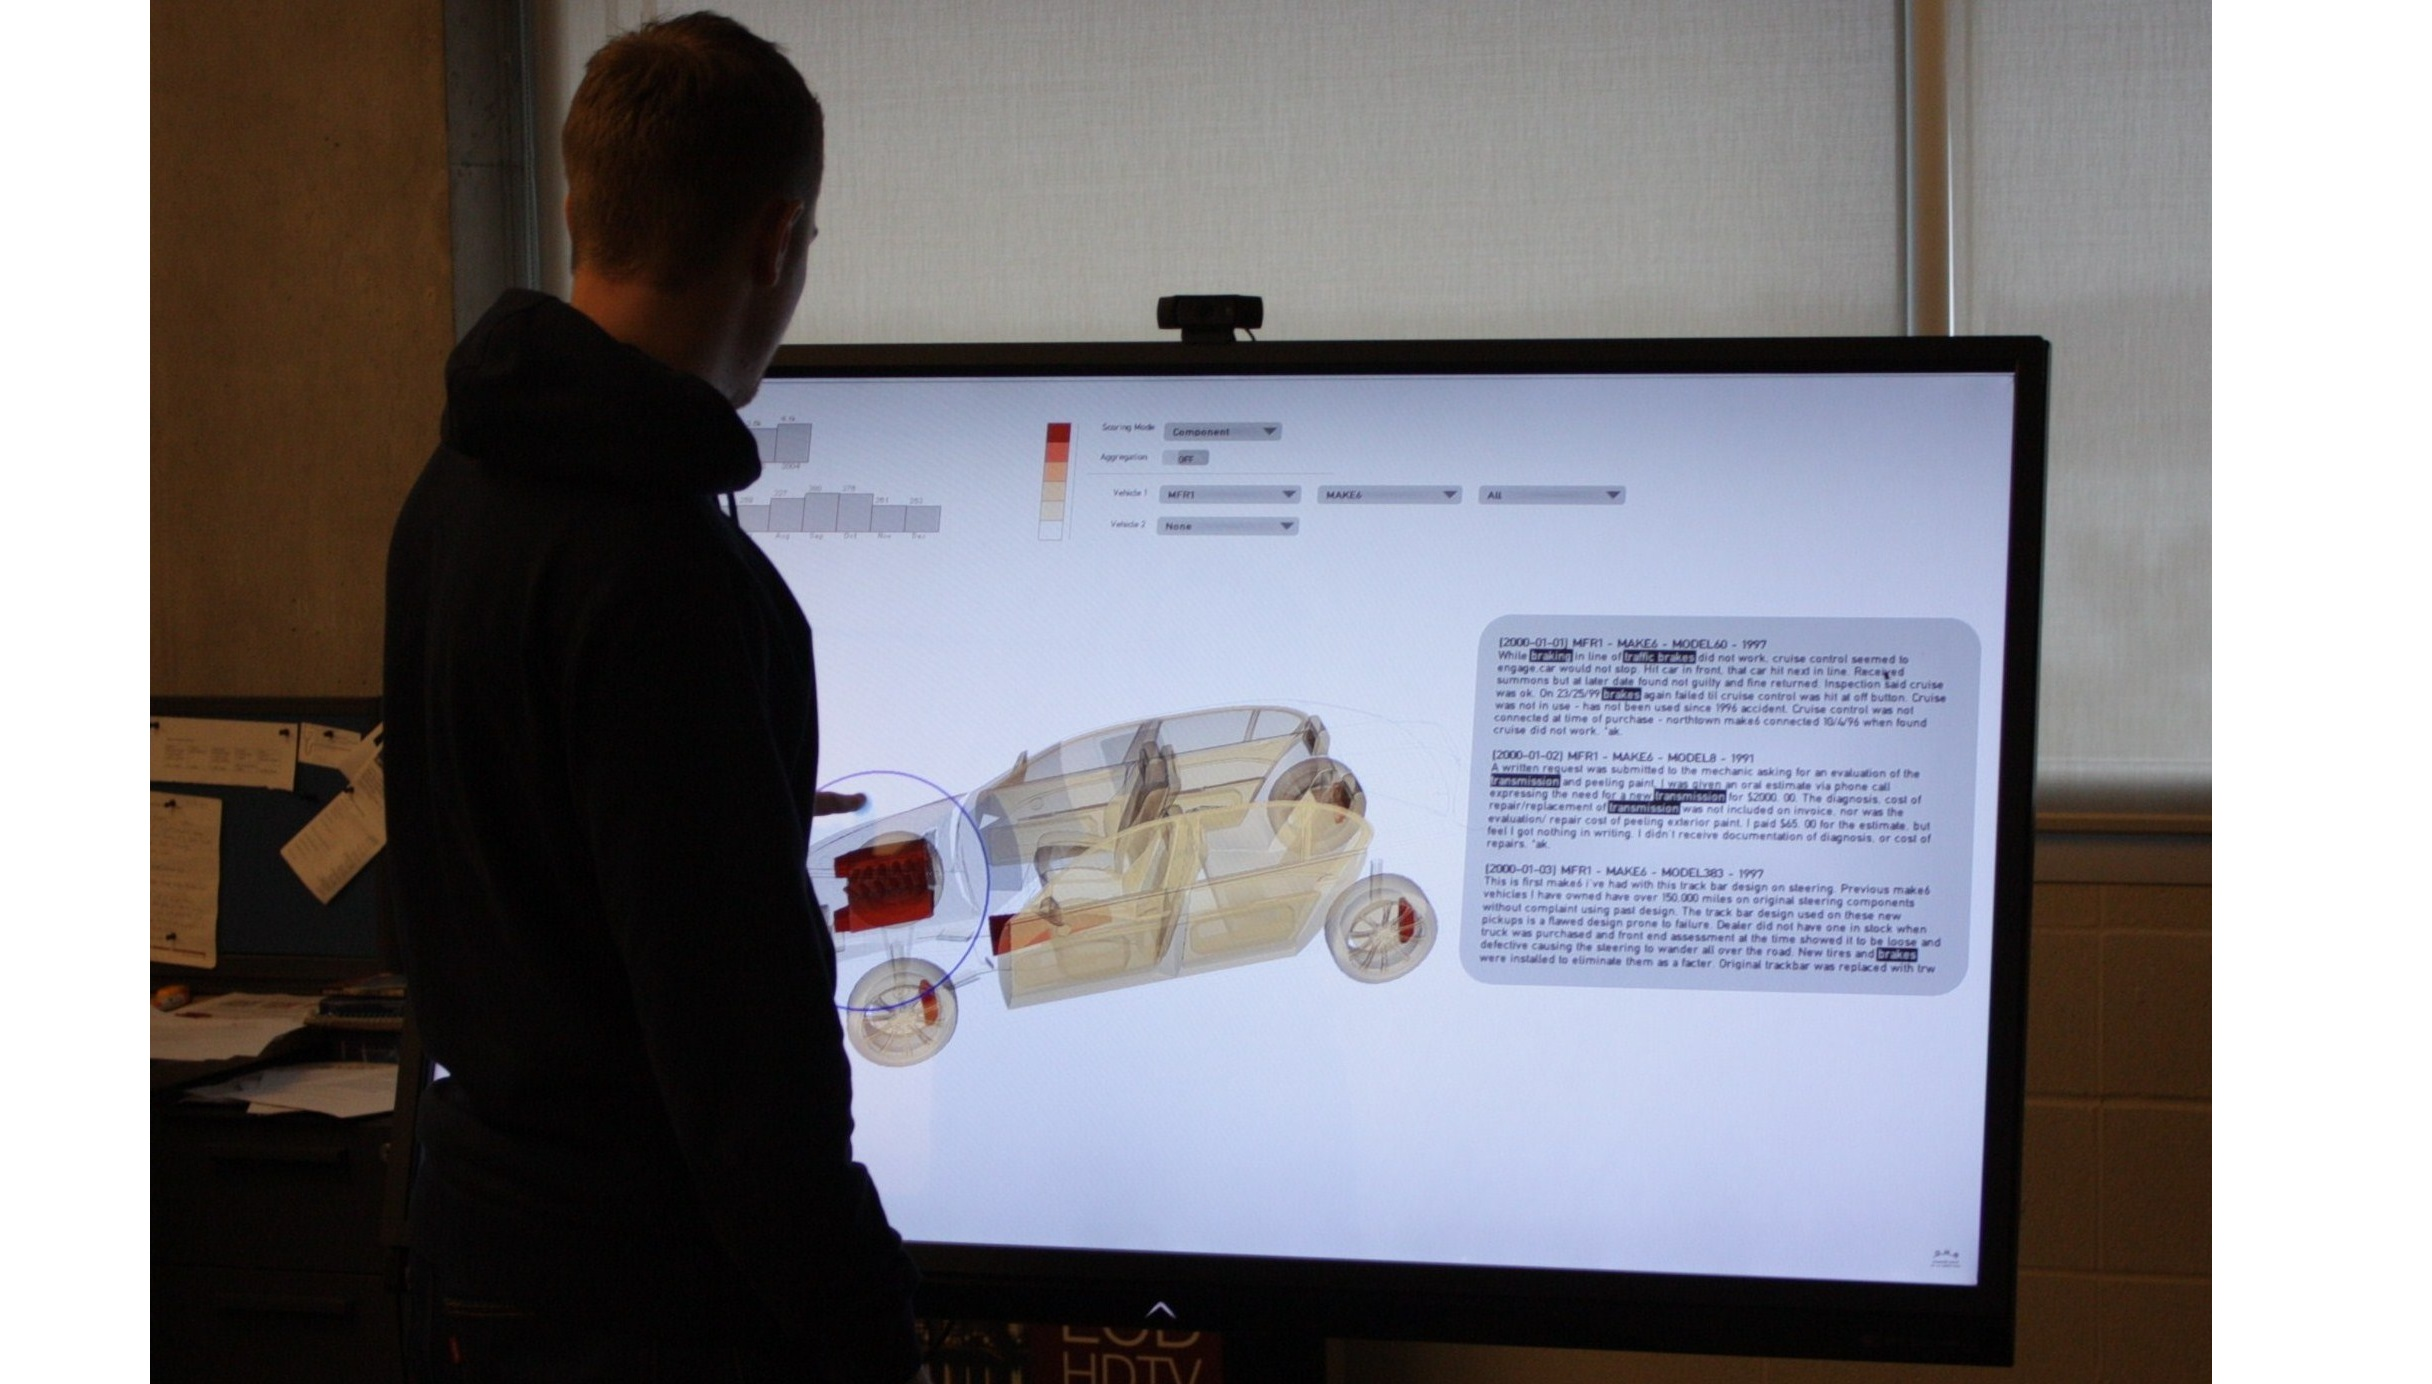
\includegraphics[width=\columnwidth]{erik_touch.JPG}  
	 \caption[Study Setup.]{A study session running on a 60 inch display with touch sensor overlay.}
	 \label{figure:study}
	\end{figure} 
	% ==============   


The study took place in a controlled lab environment. The visualization ran on
a 60 inch display fitted with a PQLabs infrared sensor overlay capable of
multitouch recognition. To avoid personal bias that may came from prior domain
knowledge, known identifiers were removed and replaced with placeholders.
For example the model ``Civic'' was replaced with ``Model1.'' The dataset for
the study itself includes the top four occurring manufacturers, and we used a time
frame between 1997 and 2004. Two pilot studies, both with lab members, were
conducted beforehand to ensure the study was appropriate, and allowed us to
tweak usability issues. Our setup can be seen in Figure \ref{figure:study}.

Each session was recorded on video, and touch interactions were
logged by the system. Each participant was compensated with a \$10 gift
certificate for their effort. Our complete study procedure can be found in Appendix A.


After a brief tutorial on how to interpret the visualization and how to use the
interface, participants were asked to perform three sets of tasks. The first set
consists of warm-up exercises aimed to help participants become familiar with the 
interactions (these are excluded from our analysis). Next came a set of
focused tasks with specific answers, they are intended to indicate whether the
\threed visualisation can be accurately perceived. For example, one question may
be ``Select the most complained about component in the year 1999.'' Finally,
the third set of questions is subjective in nature and has open-ended answers.
For these, we presented participants with a view of the data and asked them to
describe what they see, mentioning any trends or patterns, and lastly make a
decision based on a comparison of two vehicles. For example: ``Between 1997 and
2000, which of the vehicles X and Y would you purchase and why? Assume these vehicles are
similarly priced.'' All tasks were computer-based and pre-programmed into the system, 
the interface was reset automatically between tasks. After these tasks were completed, 
we conducted a semi-structured interview to solicit opinions from participants about their experiences.  

Each study session took approximately one hour to complete, though there were no
strict time constraints and participants were allowed to take as much time as
they wanted on any task. The same tasks were used for all
participants. 


\subsection{Data Collection}
In addition to written observations, video data and system log data were 
collected during the sessions. We used the video recordings to review 
participant's answers, in particular for the interview portions to verify 
our observations. Although not in scope of our study, the videos can also provide 
valuable implications for design, as they can show where and why participants had 
problems interacting with the system, we leave this as part of our future work. 

For the system logs, we tracked user input events that impact system states such
as changes to selections and data filters. We also tracked widget usages, when they were used and
their usage duration. The logs are used to reveal if there are any preferences and usage 
patterns.
 

% Consider rewriting this to be more specific at showing how rather than
% completion rates
\subsection{Discussion}
12 participants took part in the study, however one study session was excluded
from data analysis. The reason for the elimination was due to insufficient language skills; 
this participant had severe difficulty understanding the instructions of the tasks, 
and provided confusing and contradictory statements during the interview portion.


%Interpretation of the \threed visualization seemed to be fairly accurate for
%simple scenarios, while more complicated target acquisition tasks that required
%multiple steps yielded mixed results. The first two tasks asked
%participants to directly identify the mostly significant outliers, to accomplish
%these tasks, participants were to visually identify the outlier \threed
%component and select it. There were no restrictions on their method of
%selection. In total, 8/11 and 10/11 answered correctly, however, one participant
%who selected the incorrect entity later stated that the selection was based on
%personal opinion rather than a direct interpretation of the visualization.

In general, feedback of our visualization was favourable and most tasks were
completed reasonably well, in the sense that the conclusions drawn by the
participants were derived based on findings from using our system. There are a
few exceptions: some participants did not correctly respond to the focus
questions that asked them to identify outliers (3/11 and 1/11). This may partly
be attributed to initial unfamiliarity with what the visualization is trying to
show, as one participant (P5) revealed later that the first few answers were not
based on the visualization, but rather on personal opinion about automotive
vehicles. The other exception was the third task, which asked participants to identify
which of the four manufacturers used in the study had the highest engine
complaints. To complete the task, participants had to look at each
manufacturer one-by-one, or carry out a series pairwise comparisons to find the
maximum. We believe the complexity of having to memorize multiple states likely
contributed to the incorrect answers, in total five participants chose the correct
manufacturer. 

The interpretations of co-occurrence relationships were also mixed. In these
tasks, we asked the participants to identify the components that failed when
component X failed. We expected the participants to select X and then identify
the remaining entities in the visualization. However, we found that three participants
had difficulties understanding the co-occurrence concept. We are unsure whether
this is due to insufficient explanations at the start of the study, or the fact
that the same colouring scheme is used for both occurrence co-occurrence caused
the confusions. Somewhat unexpectedly, two participants noted that document
widget also shows co-occurrences in textual form, and read the documents
directly instead of using the \threed visualization.

Analysis of subjective tasks showed that participants generally had no problems
in accomplishing what was asked. For the task regarding trend analysis, most
attention was on the heatmap widgets. Five participants explicitly mentioned
outlier months in particular vehicle components over the twelve months period
that they found to be peculiar. three participants made note of possible seasonal trends,
such as winter months usually had higher number of complaints. The remaining three 
participants did not observe any specific patterns or outliers. 

For the comparison task of picking a reliable vehicle, the participants
focused on the \threed visualization. Six participants made the choice based on
preconceived notions of which components are more vital than others. For example,
some chose solely based on which vehicle had a lower rate of engine failures. Four
chose based on the sheer number of different components that failed. The
remaining lone participant was not able to make a choice but was able to
correctly interpret the visualization, mentioning each vehicle's problems
and that neither one was desirable. One participant did not directly use the
comparison function; rather each vehicle was examined one at a time.


 
% Usage data chart
% \begin{figure}
% \begin{tikzpicture}
% \begin{axis}[ 
%     width=13cm,
%     height=8cm,
%     bar width=0.2cm,  
%     ybar=0,
%     ymin=0,
%     symbolic x coords={P1, P2, P3, P4, P5, P6, P7, P8, P9, P10, P11},
%     xtick=data, 
%     legend style={at={(1.25, 0.9)}},
%     area legend,
%     ylabel=seconds
%     ] 
%     \addplot[ybar,fill=blue!75] 
%        coordinates { (P1,85) (P2,172)(P3,106) 
%                      (P4,5)  (P5,11) (P6,96)
%                      (P7,90) (P8,90) (P9,22)
%                      (P10,19) (P11,23)
%        }; 
%     \addplot[ybar,fill=red!25] 
%        coordinates { (P1,160) (P2,4)  (P3,169) 
%                      (P4,45)  (P5,83) (P6, 45) 
%                      (P7,0)   (P8,62) (P9,54)
%                      (P10,19) (P11,143)
%        };
%     \legend{Lens, 3D Scene}    
% \end{axis}
% \end{tikzpicture}
% \caption{Time spent on Lens and 3D Scene.}
% \label{chart:usage}     
% \end{figure}
%   
%    
% In terms of interaction with the system, we observed three different
% interaction styles. One group (P2, P7) used the lens almost exclusively
% as their primary navigational tool. The second group (P4, P5, P11) were the
% opposite and used direct manipulations to rotate and zoom the \threed model to
% access different components. The last group used a combination of both lens
% widget and direct manipulation. A chart showing the distributions of time spent
% on each widget can be see in Figure \ref{chart:usage}.

    % === Figure === 
	\begin{figure}
	 \centering  
	 \includegraphics[width=\columnwidth]{timechart5.png}  
	 \caption[Log Visualization.]{Widget usage visualization for the task of comparing two vehicles.}
	 \label{figure:timechart}
	\end{figure}
	% ============== 

In Figure \ref{figure:timechart}, we present a summary of the interaction logs
for the task of comparing two different types of vehicles. In this task
participants were free to use any widget they want to investigate which of the
two vehicles is more reliable. From the figure, we see that participants first
remove irrelevant data using the filters, then they either interact with 
the lens widget or directly with the \threed scene to explore the visualization.
The navigation actions were mostly executed in short bursts, followed by an idle
period. This behaviour appears to correspond to finding interesting data and
then spending time to asses his/her findings. We thought for most participants
the lens widget would be used only after the \threed model is moved into a
desired orientation, however this is not supported by the logs. The participant
strategies seem to group in to three types: use of both the \threed scene and
the lens widget for exploration (P3, 6, 8, 9, 10), only the lens widget (P2, 7),
and only the \threed scene (P1, 4, 5, 11). Surprisingly, participants did not
make use of the document during this task. Further investigation of the role of
full-text details can play in decision-making using d-NPR is warranted.


 
\subsection{Participant Feedback}
Participants enjoyed using the \threed visualization along with the lens widget.
Several participants made explicit comments with regards to the usage of a
familiar form factor through the \threed model. \emph{``Nicer to look at a
picture than a bunch of numbers.''} (P1), \emph{``everything is in detail, very
interactive.[\ldots] The visual, is self-explanatory''} (P8), \emph{``I can see
clearly each part in the car, so I know what to choose''} (P6), and \emph{``it is
relatable, I've been in cars and I've had the opportunity to see some of the
components.''} (P2). Using the lens widget for dynamic focusing of interesting
data was voiced by several participants: \emph{``kind of cool, being able to
dissect with it.''} (P1) and \emph{``You can zoom in to the parts that you
cannot really understand, for example the transmission.''} (P7).

Interaction with the heatmap had the most negative reactions. Four participants
thought the heatmap provided too much detail, they argued that an ordinary
consumer would not care for trend details, they would only care about the
overall verdict of whether a component is reliable or not. In particular, P11
suggested using a pie-chart or a bar-chart for each component in comparison view
rather than using a heatmap.  The design implication here may be to provide
different levels of granularity that can be dynamically adjusted. The lack of
labelling on the heatmap was raised by three others, as it made it more
difficult to identify individual months. Also the additional colour encoding
that is applied to the border of each cell in comparison mode made it more
difficult to distinguish the different severity levels. 

Overall, we observed several interaction issues. A few participants tried to
use the lens' depth function to access occluded objects, however we noted that
there were difficulties making fine adjustments, especially if the objects are
close to each other. Problems interacting with the touch surface was a general
concern voiced during the study, in particular we observed problems with
selection/deselection and manipulation of the filter widgets. The touch issues 
are exemplified in Figure \ref{figure:timechart}, note the time duration spent
on the filters, also note the rapid succession of selection actions which may
indicate problems with our multitouch heuristics. Despite these problems,
participants seem to enjoy using the visualization: \emph{``even though there
are some interaction problems, it just looks really good~``} (P10).

%The \threed visualization and lens mechanism received the most positive
%feedback. Participants liked how the \threed model can be used to provide 
%an overview showing all the entities. They also found it fun and enjoyed using
%the lens to focus in on specific regions, particularly for revealing objects
%that were unknown to them before.

%Interaction with the heatmap widget had the most negative reactions. Four
%participants thought the heatmap widget provided too much detail, they argued
%that an ordinary consumer would not care for trend details, they would only care
%about the overall verdict of whether a component is reliable or not. Three other
%participants had concerns about the readability of the heatmap itself, they
%mentioned that the lack of labelling made it difficult to identify individual
%months. Also the additional colour encoding that is applied to the border of each
%cell in comparison mode made it more difficult to distinguish the different
%severity levels. Several participants tried to use the lens' depth function to access
%occluded objects, however we observed that there were difficulties making fine
%adjustments, especially if the objects are close to each other. 
  
During the interview session, we asked the participants what they would do to
improve the system, there are four ideas relating to visualizations that emerged
from the study sessions:
\begin{itemize}[noitemsep]
  \item Non-consecutive years: Allow non-contiguous selection. For
  example select the years 2000 and 2002. Several participant also mentioned it
  would be nice to make year-to-year comparisons for each entity without
  leveraging the heatmap.
  
  \item Semantic zoom for the document widget: Several participant noted that
  the text on the document widget felt overwhelming, and would be better to
  present a brief summary before diving into the full text.
  
  \item Provide entity summary: The system only shows the name of the entity,
  there are a few participants that mentioned it would be nice to add a brief
  description to what the entity is and its function.
  
  \item Regional select: Provide a shortcut to select all entities under the
  lens.
\end{itemize}
   
  
\subsection{Summary}
Our study sessions showed that in general people were able to interpret the
visualization correctly. However for complicated situations where the analysis
require multiple steps, results tend to vary. In cases like this, a different
design approach such as supporting history or breadcrumb trails may be useful.
In the open-ended tasks, we observed that participants were able to use the
visualization and various interaction widgets to help guide their analysis.

The \threed visualization itself was intuitive. There are times where we did not
sufficiently explain the interface but participants were able to correctly infer
the correct interpretation. For example P1 was able to tell which entities had higher rate
of complaints in comparison mode even though we failed to mention the encoding scheme during demo. 
The semantic relations of occurrence and co-occurrence were harder to understand, which 
came as a surprise as we did not encounter comprehension issues in our pilot studies, 
perhaps a more hands-on tutorial would have helped.

%Performance???
Overall, the receptions of using the visualization were positive; other than the
comments above, \emph{``cool''}, \emph{``relatable''}, and \emph{``that
was really neat''} were heard through out the study sessions. However, as our
study is by large exploratory and qualitative in nature, a more thorough study
that involves more complex scenarios and performance metrics may further
validate the strength of our visualization approach.


%Overall, the receptions of using the visualization system were positive;
%comments such as ``cool,'' ``relatable,'' and ``that was really neat'' were heard
%through out the study sessions. Other comments, such as ``seeing all the different angles is
%nice'' and ``even though there are some interaction problems, it just looks
%really good!'' suggested the aesthetic value in showing a non-photorealistic \threed
%representation.  
  
%%%%%%%%%%%%%%%%%%%%%%%%%%%%%%%%%%%%%%%%%%%%%%%%%%%%%%%%%%%%%%%%%%%%%%%%%%%%%%%%
% This chapter covers conclusion and future works 
%%%%%%%%%%%%%%%%%%%%%%%%%%%%%%%%%%%%%%%%%%%%%%%%%%%%%%%%%%%%%%%%%%%%%%%%%%%%%%%%
\chapter{Conclusion and Future Work}
Visualization systems help us summarize and explore the ever expanding amount of
information we live with today. In this work we address a particular problem
domain of trying to make sense of a large quantity of text documents. Unlike
traditional InfoVis systems that rely on abstract representations, we explore different ways
to encoding underlying semantics on forms that are familiar to viewers. 

In this chapter we summarize our results, the limitations of our
application, and discuss avenues for future work.

\section{Limitations}
In this thesis, we have presented a working prototype showcasing descriptive
non-photorealistic rendering techniques. However, there are still some
challenges and limitations. The limitations of our prototype fall primarily into two
categories: language processing and graphical representation. In this section we
will discuss what they are and possible solutions.

From a language perspective, our system of parsing text is quite simplistic as
we are only taking into account word frequencies. Casual relations are inferred with
co-occurring entities, however a more precise method would use grammatical
structures to infer relations. While we have made early attempt at extracting
dependency relations, it did not yield fruitful result due to many grammatically
incorrect sentences in the document text, however a different text
corpus may benefit from this approach. We also only looked at nouns, it may be
interesting to look at verbs and adjectives as well.

In terms of graphical representations, occlusion still presents an issue,
especially in densely packed areas. These areas make interactions difficult.
While the heatmaps provide an easy alternative for entity selection, it does not
solve perceptual difficulties in trying to uniquely identify an object in the
visualization. Zooming into the scene, or changing the lens' depth only
partially solve the problem as both method require very fine adjustments from
the viewer. Alternative selecting approaches, such as selecting by
severity levels or other heuristic may help. Alternative graphical techniques
such as exploded views would be able to push objects away from each other, avoiding occlusion in
the first place but at a possible risk of distorting the overall context.


\section{Conclusion}
Our main contribution in this work is an integrated approach for doing text
analytics for documents that contain both spatial and non-spatial data. We extract
physical entities from text documents and encode the abstract semantics onto 
\threed models that correspond to these entities as stylistic graphical effects, thus 
reconstructing the subject matter in a way that is familiar to the viewers. We call
our approach \emph{descriptive non-photorealistic rendering}.

In order to gauge the effects of our approach, a user study was conducted with
12 participants where they were asked to analyze NHTSA's repository of vehicle
complaint reports. Each participant were asked to perform objective and
open-ended tasks in order to give us a sense of whether the visualization can be
accurately interpreted, and whether participants can perform complex tasks using our system.
Study results showed that people were able to perform analytical tasks
within our system, and that the visualization itself was well received based on
aesthetic factors and the interactive options we provided. 


% In this thesis, we applied our methods to analyze a large collection of vehicle
% complaint reports from the NHTSA database. We leveraged WordNet database to
% create a vocabulary of vehicle entity, we then score each document based on
% occurrence and co-occurrence relations among the different vehicle entities.
% We also take into consideration time and organizational hierarchy dimensions. We
% applied the entity scores onto a \threed vehicle model using NPR techniques to
% emphasis importance. Finally we created interactive widgets for exploration of
% the dataset. Our intended audience are vehicle owners and potential consumers
% whom have a stake in the safety and reliability of their vehicles.


% As a necessary step towards validating our design and hypothesis, we ran a user
% study to see if people can accurately interpret the visualization, we also
% solicited qualitative feedback from study participants. Our study showed that
% (need results to put in here)
 

\section{Future Work}
While we have explored different mappings in terms of language and graphics,
there is another aspect that we have left unexplored. The social aspect of
computing is a prominent topic today and worthwhile for further investigation.
How one would go about annotating, sharing and searching for other people's
findings are tasks that go beyond individual analysis that can help help the
entire community.

As hinted in limitations section, more robust language processing would be very
desirable. In particular, it would be interesting to look at sentiment analysis.
The capability to quantify positive or negative connotations would be beneficial
in understanding how people perceive certain physical objects.

    % === Figure === 
	\begin{figure}
	 \centering  
	 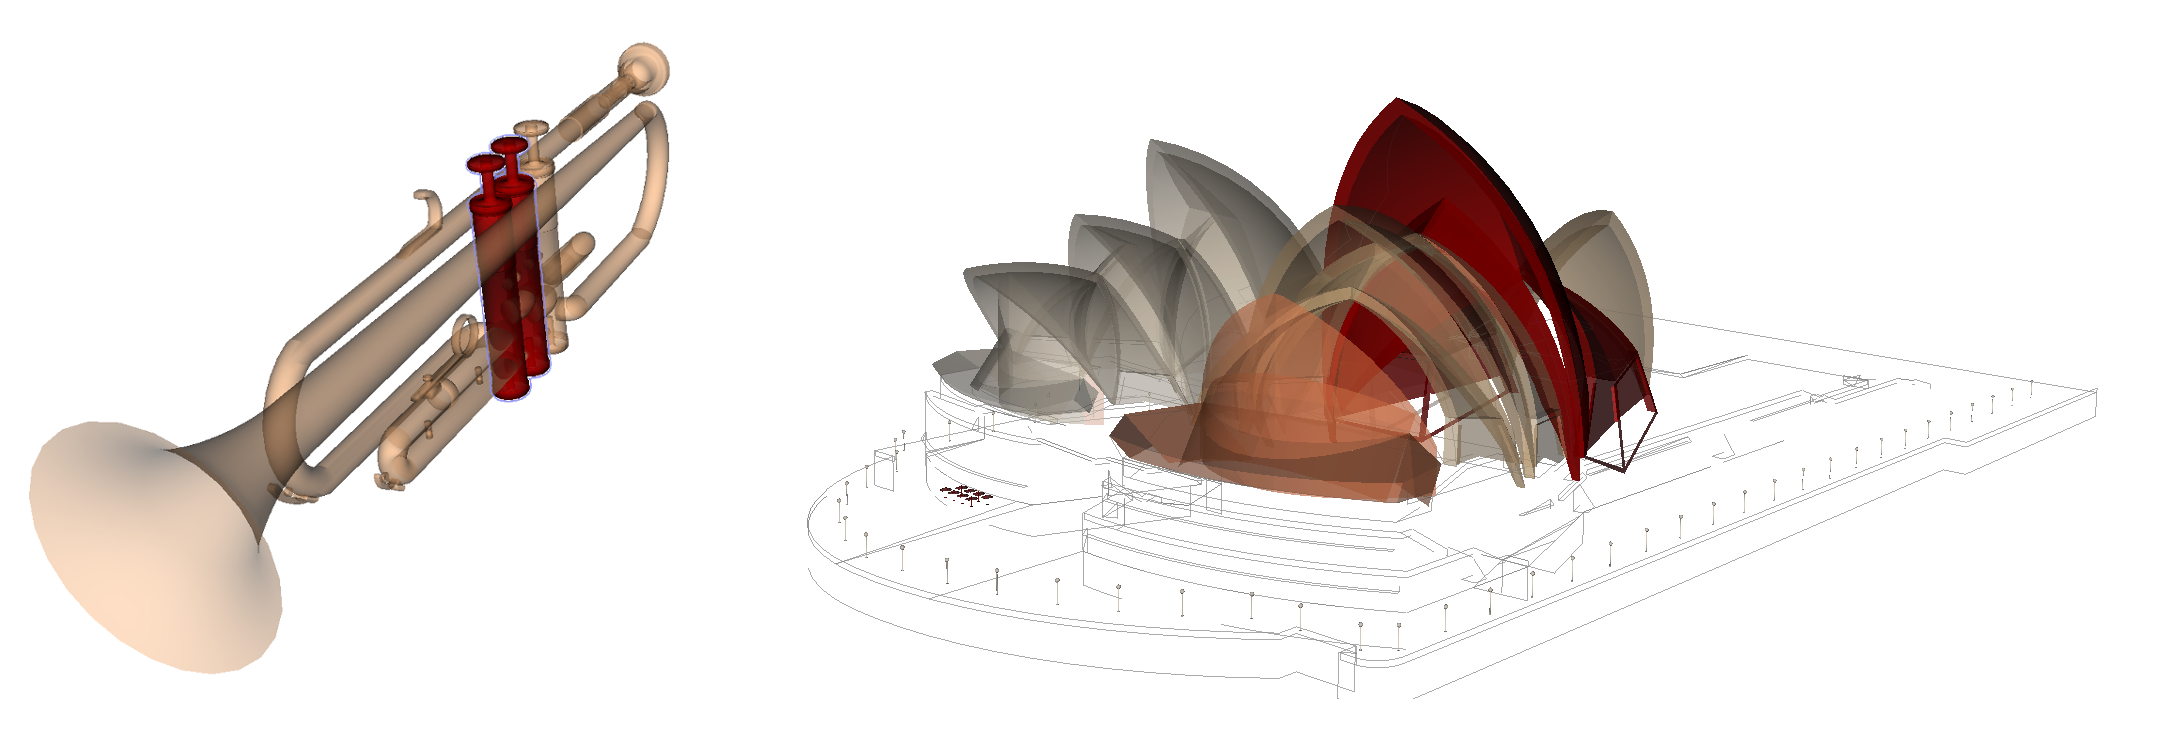
\includegraphics[width=\columnwidth]{future.png}  
	 \caption[Other Uses]{Possible usage for other domains: quality control for
	 musical instruments and building maintenance.}
	 \label{figure:future}
	\end{figure}
	% ============== 

Ambient settings is another possible area for future work, one can imaging using
camera planning algorithms to conduct a virtual tour of the entities while not
receiving input interactions. The said tour can be used to raise awareness of
particular features and highlight trends. The tour could be interrupted when a
person starts interacting with the display.

Lastly, while in this thesis we have primarily looked at the vehicle domain. Our
visualization approach is generalizable to other problems. Other analytical
tasks that relates text to physical productions may benefit from our approach. For
example see Figure \ref{figure:future}, where we show possible extensions
to look at quality control reports of a product such as a musical instrument,
and building maintenance records.




%% This adds a line for the Bibliography in the Table of Contents.
\addcontentsline{toc}{chapter}{Bibliography}
%% ***   Set the bibliography style.   ***
%% (change according to your preference)
\bibliographystyle{plain}
%% ***   Set the bibliography file.   ***
%% ("thesis.bib" by default; change if needed)
\bibliography{thesis}

%% ***   NOTE   ***
%% If you don't use bibliography files, comment out the previous line
%% and use \begin{thebibliography}...\end{thebibliography}.  (In that
%% case, you should probably put the bibliography in a separate file
%% and `\include' or `\input' it here).

%% Appendix ( User study procedure )
%%%%%%%%%%%%%%%%%%%%%%%%%%%%%%%%%%%%%%%%%%%%%%%%%%%%%%%%%%%%%%%%%%%%%%%%%%%%%%%%
% Appendix. For data files, study questions, full study results etc etc
%%%%%%%%%%%%%%%%%%%%%%%%%%%%%%%%%%%%%%%%%%%%%%%%%%%%%%%%%%%%%%%%%%%%%%%%%%%%%%%%
\appendix


%%%%%%%%%%%%%%%%%%%%%%%%%%%%%%%%%%%%%%%%%%%%%%%%%%%%%%%%%%%%%%%%%%%%%%%%%%%%%%%%
% Study questions
%%%%%%%%%%%%%%%%%%%%%%%%%%%%%%%%%%%%%%%%%%%%%%%%%%%%%%%%%%%%%%%%%%%%%%%%%%%%%%%%
\chapter{Study Procedure}

\noindent 
Research Ethics Board \#11-110 \\
\noindent
The study will consist of objective, subjective and a short interview session.
At first we will introduce the study and collect participant demographics, and
then we will train participants about the features of the prototype.
Participants will be encouraged to go through the warm up tasks to get familiar
with the visualization and interactions. Participants will then to go through
the objective, subjective rounds. We will videotape the study session to record
participant actions for later analysis. Finally we will ask participants several
interview questions to solicit their experiences using our prototype.

\noindent
Introduction
\begin{itemize}[noitemsep]
  \item Collect consent forms and distribute gift-cards
  \item Explain the purpose of the study is to gauge how well the visualization
  an be interpreted and how it can be used to support decision making tasks
  \item Explain that the study procedure consists of computer based tasks and a
  semi-structured interview
  \item Explain the NHTSA dataset
  \item Remind participants that they are not being judged based on computer
  skills, and that withdraw does not impact compensation
\end{itemize}

\noindent 
Demographic Questions
\begin{itemize}[noitemsep]
  \item Do you drive?
  \item Do you own a vehicle?
  \item Have you ever looked into automobile safety issues?
  \item Have you ever purchased a car (for yourself or someone else)?
  \item Have you ever used touch-screen interface? If so, which ones?
  \item Do you play \threed video games or otherwise use \threed graphical
  interfaces regularly?
\end{itemize}


\noindent
Demo the system to the participants, prompt participants to ask any questions
during the demo.
\begin{itemize}[noitemsep]
  \item Explain the visual encoding and \threed environment
  \item Explain occurrence and co-occurrence relations
  \item Demo the filter widgets (time filter and hierarchy filter)
  \item Demo lens, heatmap and document widgets.
  \item Explain how comparison mode works
\end{itemize}


\noindent 
Warm up tasks, these are designed for the participants to become
familiar with the visualization and the system interactions.
\begin{itemize}[noitemsep]
  \item Select years 2000 and 2001 on the year slider.
  \item Select at least two components on the \threed vehicle model.
  \item Select a vehicle component using the lens' heatmap.
  \item Use the comparison function to compare two different vehicle
  manufacturers, then select a vehicle component from the \threed vehicle model.
\end{itemize}
 


\noindent 
Objective tasks, these tasks have specific requirements and answers, these tasks
are used to gauge the accuracy of participants perception of the \threed
visualization.

\begin{itemize}[noitemsep]
  \item Select the component with the highest rate of complaint overall in the
  year 1999.
  \item Select the component with the highest rate of complaint in July and
  August, from 2000 to 2001.
  \item Which manufacturer has the highest number of engine complaints in 1998,
  select this manufacturer from the manufacturer drop down
  \item Tell us, verbally, what other components in the vehicle are associated
  with complaints about windshield and wheel? Do not change the time or the
  hierarchy filters.
  \item Find a complaint that is associated with both engine and wheel
  components. Read it out when you find it. You can use whatever widgets  you
  want to accomplish this task.
\end{itemize}


\noindent 
Subjective tasks, these tasks are open-ended. There are used to see if, and how
participants use the visualization to solve analytical problems.

\begin{itemize}[noitemsep]
  \item Which manufacturer had the least complaints in January between 1997 and
  1998? What are these complaints about?
  \item Using the lens and the heatmap widgets, observe for any trends, patterns
  or outliers in the year 1997, tell us about your findings.
  \item Between 1997 and 2000, which of the following Make would you consider to
  purchase and why? MRF1:MAKE1 or MRF2:MAKE3? Assume they are similarly
  priced.
\end{itemize}

 
\noindent
Interview questions, conducted during a semi-structured interview. These
questions are designed to solicit subject feedback about the visualization and
design improvements.



\begin{itemize}
  \item Do you find the \threed visualization intuitive and easy to read? Why or
  why not?
  \begin{itemize}
    \item Do you think the visualization is useful for showing the vital safety
    issues?
  \end{itemize}
  
  \item What do you think of the lens widget? What do you like or not like about
  it?
  \begin{itemize}
    \item Do you understand the heatmap? Do you find it intuitive and do you
    believe it is easy to spot trends and outliers?
  \end{itemize}
  
  \item Which feature of the application do you most enjoy using? Which features
  do you find the last useful for looking at reliability issues? 
  
  \item Did you encounter any issues using any of the widgets? 
  \begin{itemize}
    \item  Prompt about possible usability issues and improvements.
  \end{itemize}
  
  \item Do you have any other suggestions or feedback about the application?
\end{itemize}


\noindent
Thank the participant for coming, remind participant of right to withdraw from
the study.


\end{document}

%%%%%%%%%%%%%%%%%%%%%%%%%%%%%%%%%%%%%%%%%%%%%%%%%%%%%%%%%%%%%%%%%%%%%%
%%  End of UT-THESIS.TEX
%%%%%%%%%%%%%%%%%%%%%%%%%%%%%%%%%%%%%%%%%%%%%%%%%%%%%%%%%%%%%%%%%%%%%%
